\documentclass{TUBthesis}

%%%%%%%%%%%%%%%%%%%%%%%%%%%%%%%%%%%%%%%%%%%%%%%%%%%%%%%%%%%%%%%%%%%%%%%%%%%%
% Predefined class variables
\Title{Grapheneinbettungen und Optimierung} %title of the thesis
\Thesis{Master Thesis} %type of thesis, i.e. bachelor/master/diploma
\Author{Jonas Neukamm} %name of author
%\Uni{Technische Universität Berlin}
\MNumber{324283} %matriculation number
\Supervisor{Prof. Dr. Stefan Felsner} %name of supervisor and first referee
\Referee{Dr. Frank Lutz} %name of second referee
\Date{7.6.2019} %date of delivery
\Language{german} %choose between english and german



%%%%%%%%%%%%%%%%%%%%%%%%%%%%%%%%%%%%%%%%%%%%%%%%%%%%%%%%%%%%%%%%%%%%%%%%%%%%
% Room for definiton of additonal commands or to include additional packages.
% Please check the loaded packages in the .cls file first.
\DeclareMathOperator*{\argmax}{arg\, max}
\usepackage{blindtext}
\usepackage[T1]{fontenc}
\usepackage{lmodern}
\usepackage{pgf,tikz}
\usepackage{url}
\usepackage{mathtools}
\usepackage{enumitem}
\usetikzlibrary{patterns}
%\usepackage[demo]{graphicx}
\usepackage{caption}
\usepackage{subcaption}
%for algorithm
\usepackage[linesnumbered,ruled]{algorithm2e}
%bold symbols
\usepackage{bm}
\usepackage[textwidth=3.0cm]{todonotes}
\usepackage{capt-of}
%indicator function
\usepackage{dsfont}

%to ensure that floats stay in the subsection
\usepackage[section]{placeins}
\makeatletter
\AtBeginDocument{%
  \expandafter\renewcommand\expandafter\subsection\expandafter{%
    \expandafter\@fb@secFB\subsection
  }%
}
\makeatother

% footnotes
\usepackage[bottom]{footmisc}

% for nice looking tables
\usepackage{booktabs}
\newcommand{\ra}[1]{\renewcommand{\arraystretch}{#1}}

%for good refs
\usepackage{hyperref}
\usepackage{cleveref}
\usetikzlibrary{arrows}

\newcommand\myText[1]{\text{\scriptsize\tabular[t]{@{}l@{}}#1\endtabular}}


%%%%proof: instead of proof.
\usepackage{xpatch}
\makeatletter

\xpatchcmd{\proof}{\@addpunct{.}}{\@addpunct{:}}{}{}

\AtBeginDocument{\xpatchcmd{\@thm}{\thm@headpunct{.}}{\thm@headpunct{}}{}{}}
\makeatother
% Math operators in correct font
\DeclareMathOperator{\vol}{Vol}
\DeclareMathOperator{\conv}{conv}
\DeclareMathOperator{\pos}{pos}
\DeclareMathOperator{\interior}{int}



%bigger than cdot, smaller than bullet \bigcdot
\makeatletter
\newcommand*\bigcdot{\mathpalette\bigcdot@{.5}}
\newcommand*\bigcdot@[2]{\mathbin{\vcenter{\hbox{\scalebox{#2}{$\m@th#1\bullet$}}}}}
\makeatother

 %For better figure placement
\usepackage{wrapfig}
%
% Improved float placement parameters.
%
% From http://mintaka.sdsu.edu/GF/bibliog/latex/floats.html

% Alter some LaTeX defaults for better treatment of figures:
% See p.105 of "TeX Unbound" for suggested values.
% See pp. 199-200 of Lamport's "LaTeX" book for details.
% General parameters, for ALL pages:
\renewcommand{\topfraction}{0.95}	% max fraction of floats at top
\renewcommand{\bottomfraction}{0.95}	% max fraction of floats at bottom
% Parameters for TEXT pages (not float pages):
\setcounter{topnumber}{3}
\setcounter{bottomnumber}{2}
\setcounter{totalnumber}{4}     % 2 may work better
\setcounter{dbltopnumber}{2}    % for 2-column pages
\renewcommand{\dbltopfraction}{0.9}	% fit big float above 2-col. text
\renewcommand{\textfraction}{0.07}	% allow minimal text w. figs
% Parameters for FLOAT pages (not text pages):
\renewcommand{\floatpagefraction}{0.7}	% require fuller float pages
% N.B.: floatpagefraction MUST be less than topfraction !!
\renewcommand{\dblfloatpagefraction}{0.7}	% require fuller float pages


% For analysis
\usepackage{tikz,pgfplots}

\begin{document}

\chapter{Grundlagen}\label{pre}

Wir werden uns in dieser Arbeit hauptsächlich mit einfachen planaren Graphen beschäftigen, also solchen die keine Mehrfachkanten und Schleifen besitzen und für die kreuzungsfreie Zeichnungen, beziehungsweise Einbettungen, in der Ebene existieren. Sei $G = (V,E)$ ein Graph bestehend aus der Menge der Knoten $V$ und der Menge der Kanten $E \subseteq ( \,V \times V ) \,$. Eine Kante $e=(u,v)$ verbindet die beiden Knoten $u$ und $v$. Einen Graphen $G$, definiert als Kombination der Mengen von Knoten und Kanten nennen wir auch einen \textit{kombinatorischen} Graphen. Ein Pfad von $u$ nach $v$ ist eine Folge von Kanten $\{(u,w_1),(w_1,w_2),\ldots,(w_k,v)\} \subset E$ die $u$ und $v$ verbindet. Mit dem Grad deg$(v)$ eines Knoten meinen wir die Anzahl der adjazenten Kanten, der Kanten die $v$ als einen Endpunkt haben.

Eine Einbettung (oder Zeichnung) eines Graphen in der Ebene ist eine Abbildung $m:G\to\mathbb{R}^2$ die die Kanten und Knoten kreuzungsfrei in die Ebene zeichnet. Einen planaren Graphen zusammen mit einer möglichen kreuzungsfreien Einbettung in der Ebene bezeichnen wir als \textit{ebenen Graphen}. Für einen ebenen Graphen können wir, zusätzlich zu den Knoten und Kanten, auch die Menge der Gebiete (engl. faces) $F$ betrachten, das heißt die durch die Kanten und Knoten begrenzten Regionen in der Ebene. Wir bezeichnen das unbeschränkte Gebiet als das \textit{äußere} Gebiet. Wir können den Begriff der Einbettung von $G$ auch etwas weiter fassen und mit diesem nur die Definition der Menge der Gebiete $F$ von $G$ und eines äußeren Gebietes $f_{aus} \in F$ meinen, sodass mindestens eine planare Zeichnung mit diesen Gebieten existiert. Wir nennen dies auch eine \textit{kombinatorische} Einbettung. Die kombinatorische Einbettung bildet eine Äquivalenzklasse aller möglichen Zeichnungen von $G$. In ihr enthalten sind alle Zeichnungen von $G$ deren Gebiete (inklusive dem Äußeren) denen der kombinatorischen Einbettung entsprechen. Wir werden im Verlauf der Arbeit, wenn wir von Einbettung reden, manchmal eine spezifische Zeichnung und manchmal ihre Äquivalenzklasse meinen, die Bedeutung sollte sich jedoch aus dem Kontext ergeben.

\section{Geradlinige Dreiecks-Darstellungen (SLTRs)}

Wir werden uns in dieser Arbeit mit Möglichkeiten auseinandersetzten, geradlinige Dreiecks-Darstellungen für planare Graphen zu finden. Die englische Bezeichnung der geradlinigen Dreiecks-Darstellungen lautet straight line triangle representation, kurz SLTR. Die nächste Definition formalisiert diese Darstellung.

\begin{definition}[SLTR]\label{defsltr}
Eine Zeichnung eines ebenen Graphen $G$ wird \textit{SLTR} genannt falls gilt:
\begin{itemize}
\item[S1] Alle Kanten sind Segmente von Geraden.
\item[S2] Alle Gebiete, inklusive dem Äußeren, sind nicht-degenerierte Dreiecke.
\end{itemize}
\end{definition}

\begin{figure}[h]
	\centering
  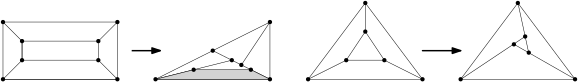
\includegraphics[width=0.95\textwidth]{sltr-example.png}
	\caption{Links einer der beiden 3-zusammenhängenden Graphen mit acht Knoten ohne SLTR und rechts ein Graph mit einer möglichen SLTR.}
\end{figure}

Für die weiteren Betrachtungen ist es nützlich die drei Knoten $\{a_1,a_2,a_3\}$, die das äußeren Gebiet berühren, gesondert zu betrachten. Wir nennen sie die \textit{Aufhängungen} von $G$. Die Knoten $a_1,a_2$ und $a_3$ sind dann die designierten Ecken des äußeren Gebietes einer möglichen SLTR. Einen Graphen zusammen mit einem äußeren Gebiet und festen Aufhängungen als Paar zu behandeln ist sinnvoll, wie in Beispiel \ref{bsp1} zu sehen sein wird.

\begin{example}\label{bsp1}
Es existieren planare Graphen, von denen manche Einbettungen SLTRs zulassen, andere jedoch nicht. Betrachten wir den planaren Graphen mit zehn Knoten aus Abbildung \ref{10_example}. Mit rot und grün sind die beiden Gebiete markiert die jeweils einmal als das äußere Gebiet festgelegt wurden. Die kombinatorische Einbettung auf der rechten Seite lässt zu dieser Wahl des äußeren Gebietes keine SLTR zu. Das nicht dreieckige Gebiet ist grau eingefärbt. Zu Auswahl auf der linken Seite existiert hingegen eine. Dies ist der kleinste 3-zusammenhängende kombinatorische Graph, der diese Eigenschaft hat.

\begin{figure}[h]
\centering
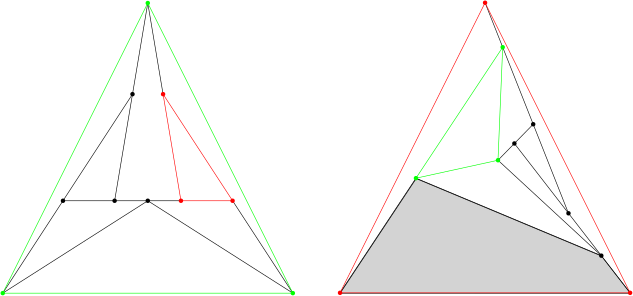
\includegraphics[width=0.7\textwidth]{10_example.png}
\caption{Zwei topologische Einbettungen des (kombinatorisch) gleichen planaren Graphen, wobei die linke keine SLTR zulässt.}
\label{10_example}
\end{figure}

\end{example}

Bevor wir zur ersten Proposition kommen werden wir die Klasse der planaren Graphen, die wir betrachten wollen etwas weiter einschränken. Dabei hilft uns die nächste Definition.

\begin{definition}[intern-k-zusammenhängend]\label{int_3_con}
Ein Graph $G$ ist zusammenhängend falls für alle Knoten $u,v$ ein Pfad von $u$ nach $v$ existiert. $G$ ist \textit{k-zusammenhängend}, falls er nach der Entfernung von $k-1$ beliebigen Knoten weiterhin zusammenhängend ist. Sei $G$ eben mit den Aufhängungen $\{a_1,a_2,a_3\}$, weiter sei $a_\infty$ ein zusätzlicher Knoten eingefügt im äußeren Gebiet. Dann ist $G$ \textit{intern k-zusammenhängend}, falls $G+a_\infty\coloneqq(V\cup\{a_\infty \},E\cup \{(a_1,a_\infty),(a_2,a_\infty),(a_3,a_\infty)\})$ k-zusammenhängend ist.
\end{definition}

Die nächste Präposition enthält eine erste notwendige Bedingung für die Existenz von geradlinigen Dreiecksdarstellungen (SLTRs).

\begin{proposition}\cite[Proposition 1.2]{af13}
Sei $G$ ein ebener Graph mit den Aufhängungen $\{a_1,a_2,a_3\}$ als äußere Ecken einer SLTR. Weiter gelte für alle Knoten $v\in V \backslash \{a_1,a_2,a_3\}$ deg$(v) \geq 3$. Dann ist $G$ intern-3-zusammenhängend.
\end{proposition}

\begin{proof}
Sei $\Delta$ die SLTR von $G=(V,E)$. Angenommen es existiert eine Menge $U \subseteq V$ in $G$ mit $|U| = 2$, deren Entnahme $G$ in nicht zusammenhängende Komponenten trennt. Wir werden zeigen, dass jeder Teil von $G\backslash U$ eine der Aufhängungen enthält und somit $G + a_\infty$ nicht von $U$ getrennt wird. Da $G$ intern-3-zusammenhängend ist können nur die Aufhängungen $a_i$ Grad zwei haben. Sei $K$ eine der Komponenten von $G\backslash U$. Betrachte $K\cup U$ als induzierten Teilgraphen von $G$. Falls $K\cup U$ ein Pfad ist, also nur Knoten von Grad zwei oder eins enthält, dann kann nur $K=\{a_i\}$ gelten.

Falls $K\cup U$ kein Pfad ist, betrachte die konvexe Hülle von $U \cup K$ in $\Delta$. Mindestens drei der Ecken von $U \cup K$ haben Außenwinkel grösser als $\pi$ (an diesen Ecken befinden sich Knoten aus $U \cup K$). Zwei dieser Winkel können an den Knoten aus $U$ liegen, aber der dritte muss ein Winkel sein, der schon in $\Delta$ existiert. Es handelt sich somit um eine Aufhängung.
\end{proof}

\begin{remark}
Für innere Knoten von Grad 2 in einer SLTR müssen die beiden angrenzenden Winkel gerade sein. Somit kann man diese Knoten durch eine gerade Kante zwischen ihren Nachbarn ersetzen und den resultierenden Graphen betrachten. Knoten von Grad eins können nicht existieren, da sie nicht aus dem Rand eines Dreiecks liegen können. Wir werden somit von nun an nur intern-3-zusammenhängende Graphen mit Aufhängungen betrachten, da alle anderen Graphen, die eine SLTR zulassen, auf diese reduziert werden können.
\end{remark}

Für 3-zusammenhängende planare Graphen mit mehr als drei Knoten ist die kombinatorische Einbettung nach Hassler Whitney bis auf Wahl des äußeren Gebietes eindeutig \cite{whitney32}. Zusammen mit der nächsten Proposition definiert somit die Wahl von Aufhängungen $\{a_1,a_2,a_3\}$, die in mindestens einem gemeinsamen Gebiet liegen, ein eindeutiges äußeres Gebiet $f_{aus}$.

\begin{proposition}
Sei $G$ ein planarer 3-zusammenhängender Graph und $\{a_1,a_2,a_3\} \subset V$. Dann existiert höchstens ein Gebiet $f$, das adjazent zu $a_1,a_2,a_3$ ist.
\end{proposition}

\begin{proof}
Angenommen es existieren zwei Gebiete $f,f'$ die $a_1,a_2$ und $a_3$ enthalten. Dann berühren sich diese Gebiete an mehr als einer Kante (vergleiche Abbildung \ref{3_con_uni} links). Im grauen Gebiet müssen Knoten liegen, da $G$ 3-zusammenhängend ist. Wenn wir aber nun $a_2$ und $a_3$ entfernen, dann teilen wir $G$ in zwei nicht zusammenhängende Gebiete. Es kann somit nur ein Gebiet $f$ geben, in welchem die $a_1,a_2$ und $a_3$ liegen.
\end{proof}

\begin{figure}
	\centering
  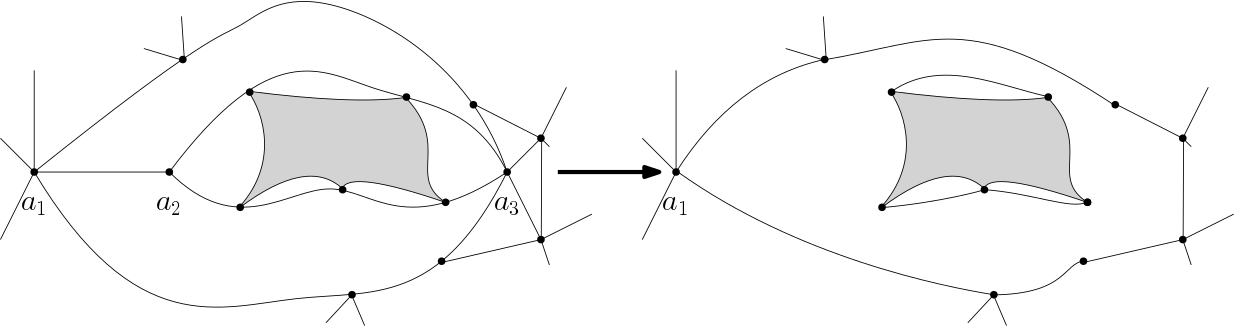
\includegraphics[width=0.95\textwidth]{3_conn_uni.png}
	\caption{Die entnehme der Knoten $a_2$ und $a_3$ trennt $G$, was zu einem Wider- spruch zum 3-Zusammenhang führt.}
	\label{3_con_uni}
\end{figure}

\begin{remark}
Wir könnten uns somit für 3-zusammenhängende planare Graphen auf die Wahl von Aufhängungen $\{a_1,a_2,a_3\}$ beschränken. Für eine kombinatorische Einbettung folgt dann ein eindeutiges äußeres Gebiet $f_{aus}$. Für nur intern-3-zusammenhängende planare Graphen gilt dies nicht. Wir betrachten somit im Folgenden ebene Graphen mit Aufhängungen $\{a_1,a_2,a_3\}$ im äußeren Gebiet.
\end{remark}

Mit den Fragen, welche notwendigen und hinreichenden Bedingungen für die Existenz von SLTRs gelten und welche algorithmischen Ansätze man bei der Suche nach einer spezifischen Darstellung verfolgen kann, werden wir uns in den nächsten beiden Kapiteln auseinandersetzen. Zuvor werden in diesem Kapitel noch einige Konzepte eingeführt, die notwendig sind, um der Argumentation zu folgen.

\section{Schnyder Woods}\label{sw}
Betrachten wir einen ebenen Graphen mit Aufhängungen $a_1,a_2,a_3$. Anschaulich handelt es sich bei einem Schnyder Wald um drei Aufspannende Bäume $T_1,T_2,T_3$, sodass jeder der Bäume $T_i$ zu seiner Wurzel $a_i$ hin gerichtet ist. Jede der Kanten wird mindestens von einem der Bäume genutzt und Kanten können von zwei der drei Bäume gleichzeitig genutzt werden.

Schnyder Wälder, im weiteren nach der englischen Bezeichnung \textit{Schnyder Woods}, wurden zuerst von Walter Schnyder eingeführt \cite{schnyder89}. Es handelt sich die um eine Färbung und Orientierung der inneren Kanten einer Triangulierung. Sie dienten der Betrachtung der von planaren Graphen induzierten Ordnungen. In einer weiteren Arbeit wurden mit ihrer Hilfe geradlinige und konvexe Einbettungen Triangulierungen auf einem $(|V|-2)\times(|V|-2)$ Gitter erzeugt \cite{schnyder90}.

Wir wollen hier die Verallgemeinerung auf 3-zusammenhängende planare Graphen durch Felsner und die zu ihnen in Bijektion stehenden Schnyder Labelings einführen \cite{felsner01}. Wir orientierten uns dabei an einem Lehrbuch von Felsner \cite{felsner12}. Für den Rest dieses Kapitels sei $G$, wenn nicht weiter spezifiziert, ein 3-zusammenhängender ebener Graph mit Aufhängungen $\{a_1,a_2,a_3\}$.

\begin{definition}[Schnyder Woods]\label{def_sw}
Ein Schnyder Wood ist eine Orientierung und Beschriftung der Kanten von $G$ mit den Labeln 1, 2 und 3\footnote{Es wird davon ausgegangen, dass die Label zyklisch sortiert sind, sodass $i+1$ und $i-1$ immer definiert sind.} (alternativ wird hier auch oft rot, grün und blau genutzt), unter Berücksichtigung der folgenden Regeln:
\begin{itemize}
\item[W1] Jede Kante ist entweder in eine oder zwei Richtungen orientiert. Falls sie bigerichtet ist, haben beide Richtungen unterschiedliche Label.
\item[W2] An jeder Aufhängung  $a_i$ existiert eine nach außen gerichtete Halbkante\footnote{Eine Halbkante ist eine Kante mit nur einem Endpunkt.} mit Label i. 
\item[W3] Jeder Knoten $v$ hat Ausgangsgrad eins in jedem Label. Um $v$ existieren im Uhrzeigersinn eine Auskante mit Label 1, null oder mehr eingehende Kanten mit Label 3, eine Auskante mit Label 2, null oder mehr  eingehende Kanten mit Label 1, eine Auskante mit Label 2 und null oder mehr  eingehende Kanten mit Label 2.
\item[W4] Es existiert kein inneres Gebiet mit einem gerichteten Zykel in einer Farbe als Rand.
\end{itemize}
\end{definition}

\begin{figure}[h]
	\centering
  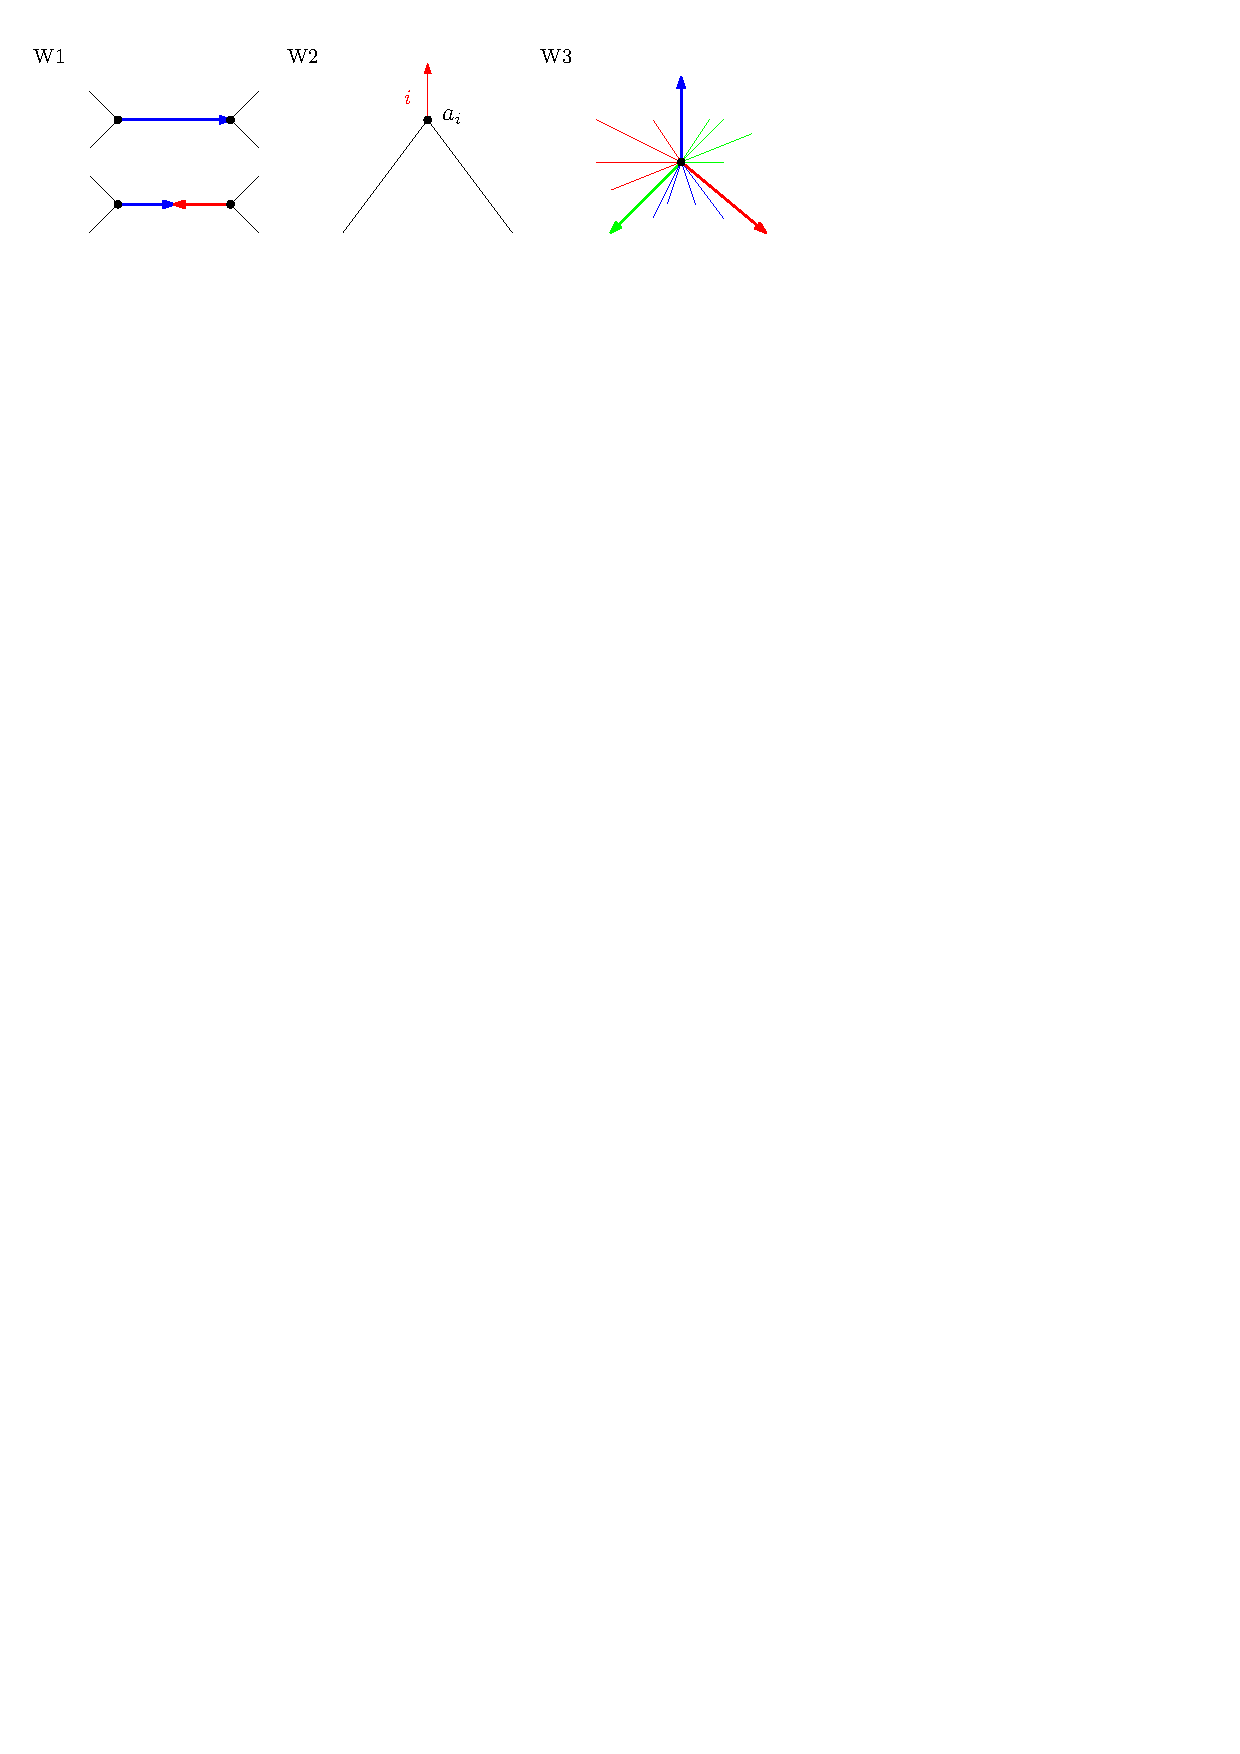
\includegraphics[width=0.9\textwidth]{schnyder_wood_def.pdf}
  \caption{Illustration der ersten drei Bedingungen für Schnyder Woods.}
\end{figure}

Analog zu den Schnyder Woods, kann man Schnyder Labelings definieren, die zu diesen in Bijektion stehen. Hier betrachten wir nicht zuerst die Kanten eines planaren Graphen sondern die Winkel an den Knoten.

\begin{definition}[Schnyder Labeling]\label{def_sl}
Ein Schnyder Labeling ist eine Beschriftung der Winkel von $G$ mit den Labeln 1, 2 und 3 (oder rot, grün und blau) unter Berücksichtigung der folgenden Regeln:
\begin{itemize}
\item[L1] Um jedes innere Gebiet bilden die Label im Uhrzeigersinn nichtleere Intervalle von 1en, 2en und 3en. Am äußeren Gebiet gilt dies gegen den Uhrzeigersinn.
\item[L2] Um jeden inneren Knoten bilden die Label im Uhrzeigersinn nichtleere Intervalle von 1en, 2en und 3en.
\item[L3] An den Aufhängungen $a_i$ haben die äußeren Winkel die Label i-1 und i+1 im Uhrzeigersinn mit der Halbkante dazwischen. Die inneren Winkel haben das Label i.
\end{itemize} 
\begin{figure}[h]
	\centering
  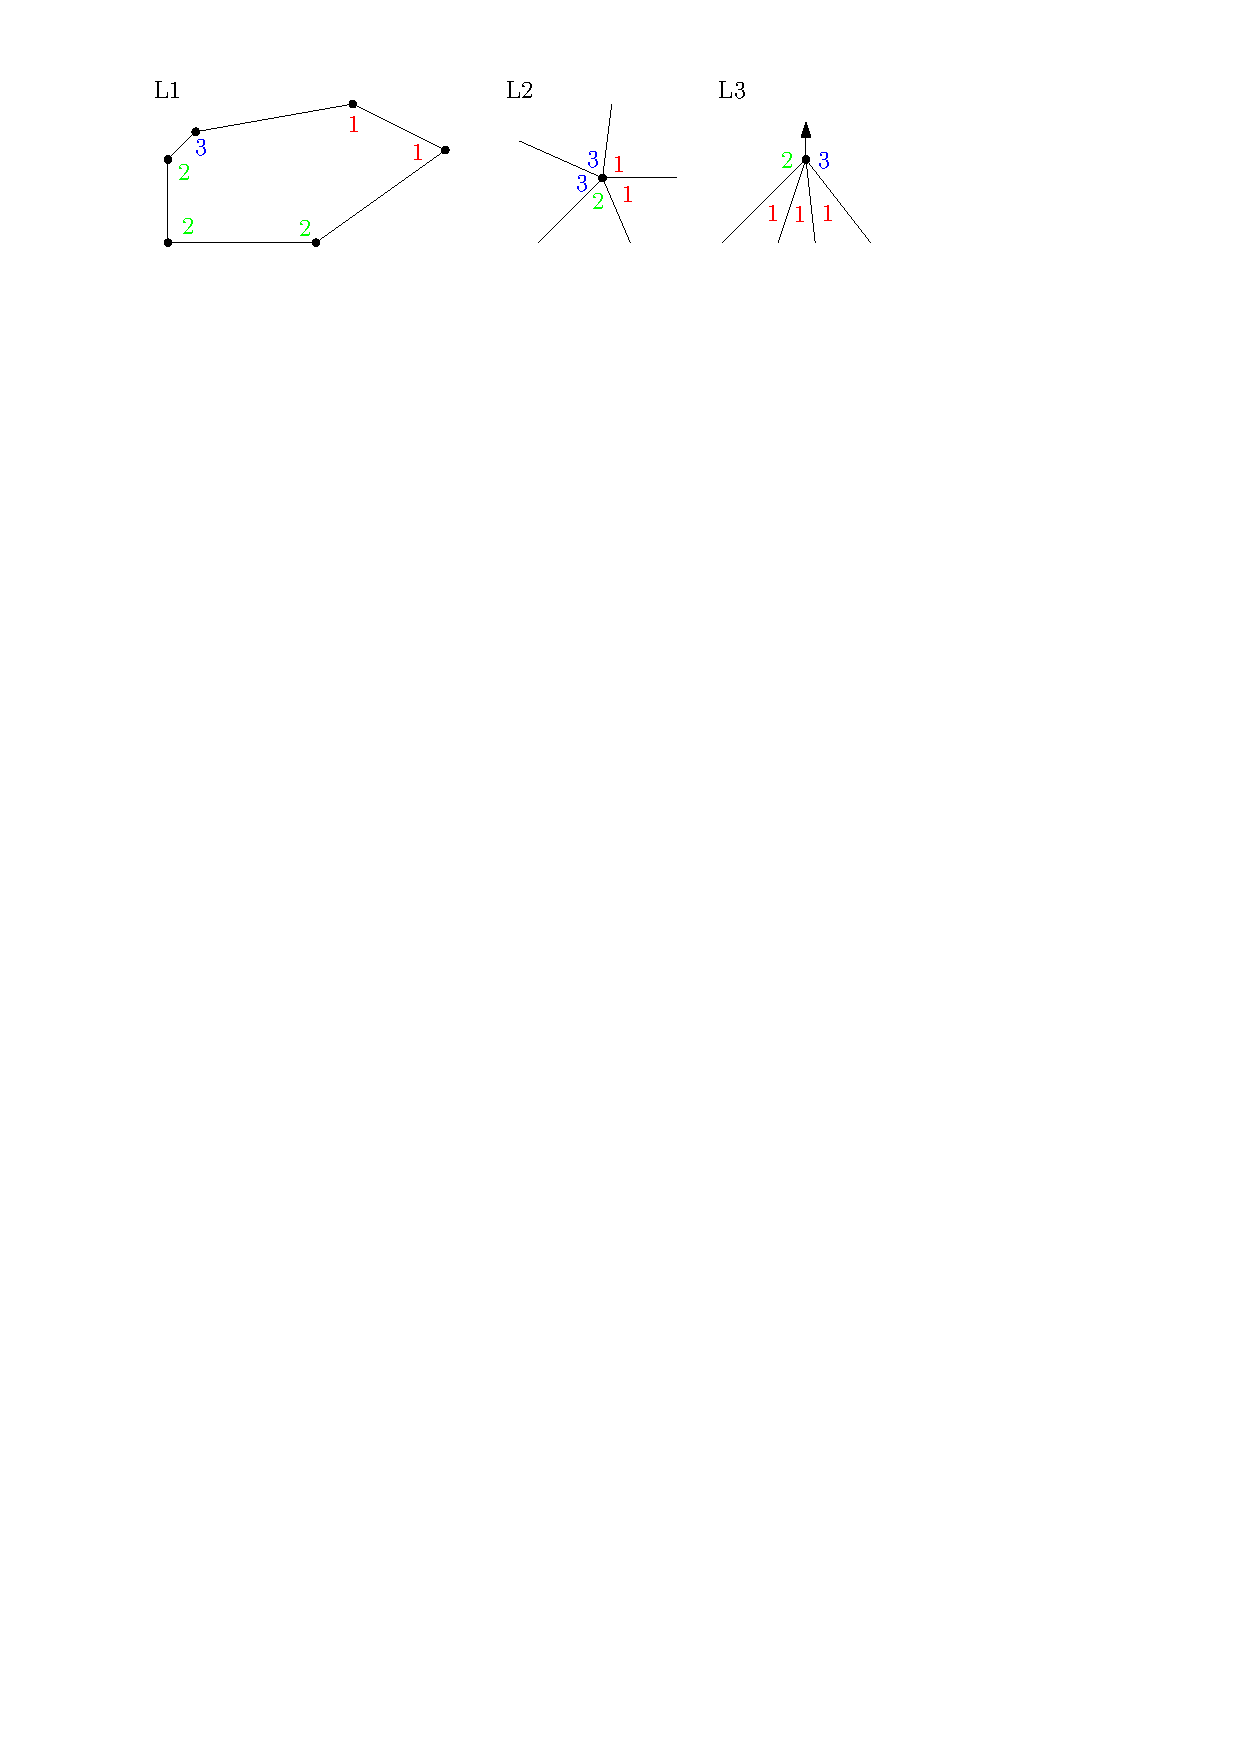
\includegraphics[width=0.9\textwidth]{schnyder_label_def.pdf}
   \caption{Illustration der drei Bedingungen für Schnyder Labelings.}
\end{figure}
\end{definition}

In Abbildung \ref{schnyder_bij} wird eine Verbindung zwischen Schnyder Woods und Schnyder Labelings illustriert. Das nächste Lemma folgt aus den Bedingungen L1 und L2.

\begin{lemma}\label{lem_sl}
Sei G ein ebener, intern-3-zusammenhängender Graph mit den Aufhängungen $a_1,a_2,a_3$ und einem Schnyder Labeling. Dann beinhalten die vier Winkel entgegen dem Uhrzeigersinn an jeder Kante die Label 1, 2 und 3. Somit hat jede Kante einen der beiden Typen in Abbildung \ref{schnyder_bij}.
\end{lemma}

\begin{figure}[h]
	\centering
  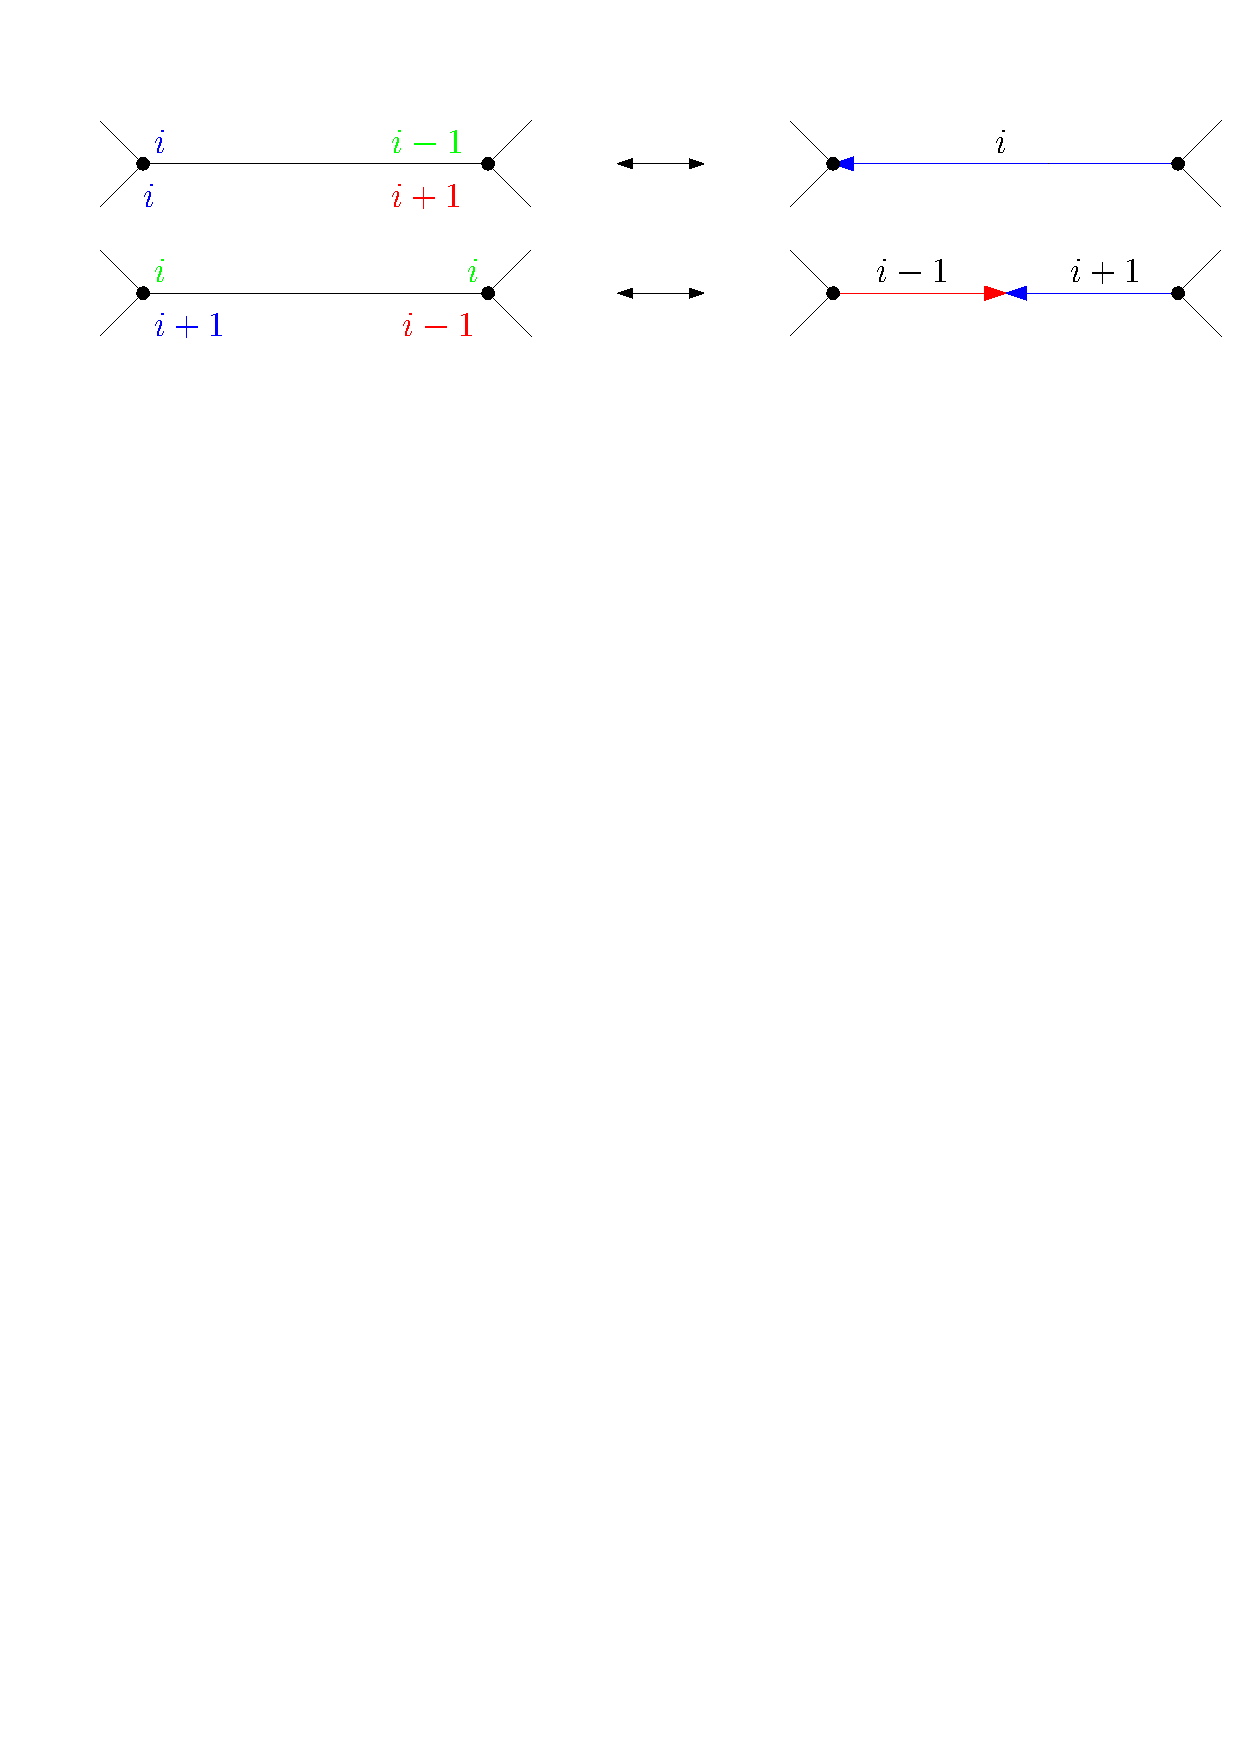
\includegraphics[width=0.9\textwidth]{schnyder_bij.pdf}
	\caption{Bijektion zwischen Schnyder Wood auf der rechten und Schnyder Labeling auf der linken Seite.}
	\label{schnyder_bij}
\end{figure}

\begin{theorem}\label{theo_schnyder_bij}
Sei G ein ebener, intern-3-zusammenhängender Graph mit den Aufhängungen $a_1,a_2,a_3$. Der in Abbildung \ref{schnyder_bij} dargestellte Zusammenhang erzeugt eine Bijektion zwischen Schnyder Woods und Schnyder Labelings auf $G$.
\end{theorem}

Dies macht es möglich, wenn für Darstellung und Verständnis sinnvoll, zwischen den beiden Strukturen hin und her zu wechseln. So kann es im Verlauf dieser Arbeit vorkommen, dass wir vom einen schreiben, aber implizit Eigenschaften des anderen meinen. Für die von uns im Folgenden betrachteten Graphen existiert mindestens ein Schnyder Wood. Dies belegt das nächste Theorem nach Ezra Miller \cite[Theorem A]{miller02}.

\begin{theorem}
Sei $G$ ein ebener Graph mit Aufhängungen $\{a_1,a_2,a_3\}$. $G$ ist genau dann intern-3-zusammenhängend, wenn ein Schnyder Wood auf $G$ mit den Ecken $\{a_1,a_2,a_3\}$ existiert.
\end{theorem}

\subsection{Einbettungen via Schnyder Woods}\label{face_counting}

Es existieren einige Anwendungen von Schnyder Woods in Bezug auf Einbettungen. Wie schon erwähnt, bezieht sich eines der ersten Resultate auf die konvexe Einbettung auf einem Gitter. Das im Folgenden skizzierte \textit{face-counting} nach Felsner (deutsch: Gebiete zählen), erzeugt eine Einbettung auf einem kleineren Gitter als nach Schnyder \cite{felsner01}. Betrachte $G$ mit einem Schnyder Wood $T_1,T_2,T_3$. Es handelt es sich bei den Bäumen $T_i$ um gerichtete Bäume mit Wurzeln in $a_i$ \cite[Korollar 2.5]{felsner12}. Von jedem Knoten $v$ aus existierten also eindeutige Pfade $P_i(v)$ zu den Aufhängungen $a_i$. Jeweils zwei der Pfade von $v$ zu den Aufhängungen haben $v$ als einzigen gemeinsamen Knoten \cite[Lemma 2.4]{felsner12}. Wir können somit zu jedem Konten $v$ drei Regionen $R_i$ definieren, die jeweils von den Pfaden $P_{i-1}(v)$ und $P_{i+1}(v)$ und dem äußeren Gebiet eingegrenzt werden\footnote{Ein Beispiel für diese Regionen findet sich in Abbildung \ref{face_counting} auf der rechten Seite.}. In jeder dieser Regionen können wir nun die eingeschlossenen Gebiete von $G$ zählen. Durch das Zählen der Gebiete in den Regionen zu $v$ lässt sich eine konvexe Zeichnung von $G$ erzeugen.

Hierzu ordnet man jedem Knoten $v$ seinen \textit{Gebietsvektor} $(v_1,v_2,v_3)$ zu, wobei $v_i$ die Anzahl der inneren Gebiete in $R_i(v)$ beschreibt. In Abbildung \ref{face_counting} sind auf der rechten Seite die Regionen von $v$ eingefärbt. Seien $\alpha_1 = (0,1),\alpha_2 = (1,0)$ und $\alpha_3 = (0,0)$ die äußeren Ecken unserer Zeichnung. Sie entsprechen ebenfalls den Bildern der Aufhängungen von $G$. Die Position der inneren Knoten ergibt sich nun durch die Funktion 
$$\mu: V \to \mathbb{R}^2,v\mapsto v_1\alpha_1 + v_2\alpha_2+v_3\alpha_3.$$ 

\begin{theorem}[Theorem 2.7 \cite{felsner12}]
Sei G ein ebener Graph mit einem Schnyder Wood $\sigma$ und den Aufhängungen $a_1,a_2,a_3$. Sei $(v_1,v_2,v_3)$ der, unter Berücksichtigung von $\sigma$ berechnete, Gebietsvektor von $v \in V$, mit $ v_i = \text{Anzahl der Gebiete in }R_i(v).$ Dann ist die Zeichnung $\mu(G)$ konvex.
\end{theorem}

Die mit diesen Koordinaten erzeugte Einbettung von $G$ ist planar, konvex und passt, falls $G$ 3-zusammenhängend ist, auf ein $(|F|-1)\times(|F|-1)$-Gitter \cite[Korollar 2.8]{felsner12}. Sie hat noch eine weitere Eigenschaft, die später von Nutzen sein wird und die in der nächsten Proposition festgehalten ist.  Dies ist in Abbildung \ref{face_counting} in der Mitte skizziert.

\begin{figure}
	\centering
  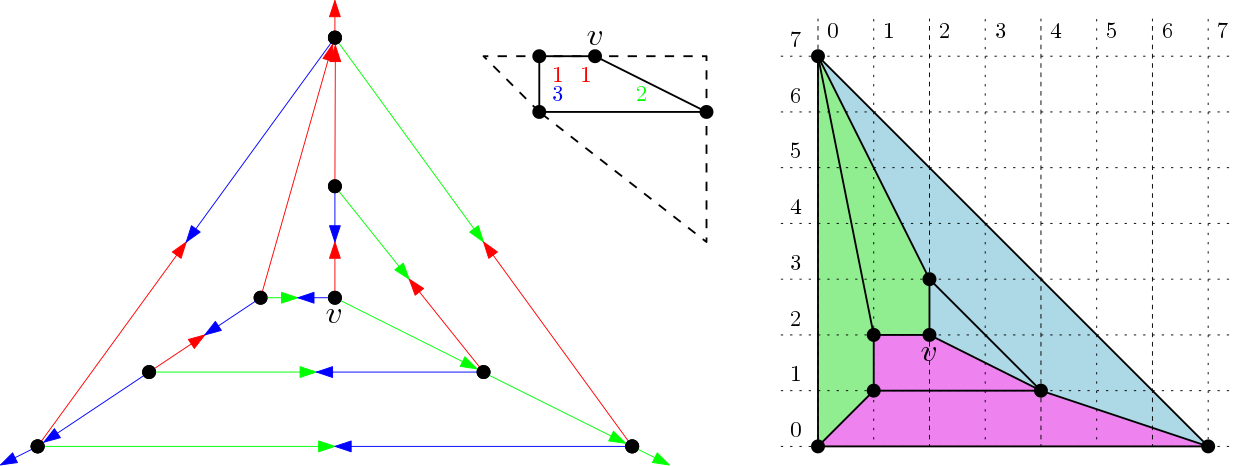
\includegraphics[width=1\textwidth]{face_counting.png}
	\caption{Eine Schnyder Wood auf $G$ und die durch face-counting erhaltene Einbettung von $G$. Die eingefärbten Gebiete sind die Regionen die den Gebietsvektor $(v_1,v_2,v_3)$ ergeben. In der Mitte ist W5 illustriert.}
	\label{face_counting}
\end{figure}

\begin{proposition}\label{w5}
Sei G ein ebener Graph mit einem Schnyder Wood $\sigma$ und den Aufhängungen $a_1,a_2,a_3$. Für $\mu(G)$, die durch face-counting erzeugte Einbettung von $G$, gilt:
\begin{itemize}
\item [W5] Die Knoten eines inneren Gebietes werden auf die Seiten eines Dreiecks mit den Seiten $c_i(\alpha_{i-1}-\alpha_{i+1})$ mit passenden Konstanten $c_i$ abgebildet. Im inneren dieses Dreiecks befinden sich keine Knoten. Die Winkel im Inneren des Gebietes an den Knoten auf der Seite $c_i(\alpha_{i-1}-\alpha_{i+1})$ haben Label $i$ im Schnyder Labeling.
\end{itemize}
\end{proposition}

\section{$\alpha$-Orientierungen}\label{alpha_orientations}

Für den Algorithmus in Kapitel \ref{main_algo} führen wir nun eine weitere zu Schnyder-Woods und Labelings in Bijektion stehende Struktur auf Graphen ein und folgen dabei wieder Felsner \cite{felsner04}.

\begin{definition}[$\alpha$-Orientierung]
Sei $G=(V,E)$ ein ungerichteter Graph und $\alpha:V\mapsto\mathbb{N}$ eine Funktion auf $G$. Eine $\alpha$\textit{-Orientierung} ist eine Orientierung der Kanten von $G$, sodass der Ausgangsgrad\footnote{Der Ausgangsgrad eines Knoten $v$ entspricht der Anzahl der adjazenten Kanten von $v$, die von $v$ weg gerichtet sind.} eines jeden Knoten $\alpha(v)$ entspricht, dass heißt $$\text{outdeg}(v) = \alpha(v).$$
\end{definition}

Um von $\alpha$-Orientierungen zu Schnyder Woods zu gelangen müssen wir Primal-Dual Graphen betrachten, die mit den nächsten beiden Definitionen eingeführt werden.

\begin{definition}[schwacher dualer Graph]
Sei $G$ ein ebener Graph. Wir definieren $G^*$, den \textit{schwachen dualen Graphen} von $G$. $G^*$ hat einen (Gebiets-)Knoten für jedes innere Gebiet von $G$. Für jede innere Kante in $G$ fügen wir eine Kante zwischen den beiden (Gebiets-)Knoten $f,f'$ in $G^*$ ein, die adjazent zu dieser Kante in $G$ sind.
\end{definition}

\begin{definition}[Primal-Dual Graph]
Betrachte einen ebenen Graphen $G$ und seinen schwacher dualen Graphen $G^*$. Der \textit{Primal-Dual Graph} $G+G^*$ ist eine Vereinigung der Graphen $G$ und $G^*$. Wenn wir $G$ und $G^*$ übereinander legen, dann kreuzen sich jeweils eine Kante aus $G$ und eine aus $G^*$. An so einer Kantenkreuzung fügen wir in $G+G^*$ einen Knoten ein und verbinden ihn mit den adjazenten Knoten aus $G$ und $G^*$. Die Menge der Knoten von $G+G^*$ besteht aus Knoten-Knoten (Knoten in $G$), Kanten-Knoten (an den Kreuzungen) und Gebiets-Knoten (Knoten in $G^*$). Kanten in $G+G^*$ existieren, sowohl zwischen inzidenten Kanten und Knoten, als auch Kanten und Gebieten in $G$. Hinzu kommen Halbkanten von den Kanten-Knoten und Knoten-Knoten am äußeren Gebiet von $G$. Wenn wir einen Knoten $f_\infty$ für das äußere Gebiet hinzufügen und die Halbkanten zu diesem verlängern spricht man vom \textit{Abschluss} von $G+G^*$. Ein Beispiel ist in Abbildung \ref{alpha_ex} a) zu sehen.

\end{definition}

Wir trennen bei der Erzeugung jede Kante in zwei Teile. Die Kanten-Knoten auf er einen und die Knoten-Knoten und Gebiets-Knoten auf der anderen Seite bilden eine Bipartition. Somit sind $G+G^*$ und sein Abschluss bipartit. Das folgende Theorem liefert eine Bijektion zwischen den Schnyder Woods auf $G$ und einer bestimmten $\alpha$-Orientierung auf dem Abschluss von $G+G^*$, die wir $\alpha_s$ nennen \cite[Propositionen 3 und 4]{felsner04}.

\begin{figure}
	\centering
	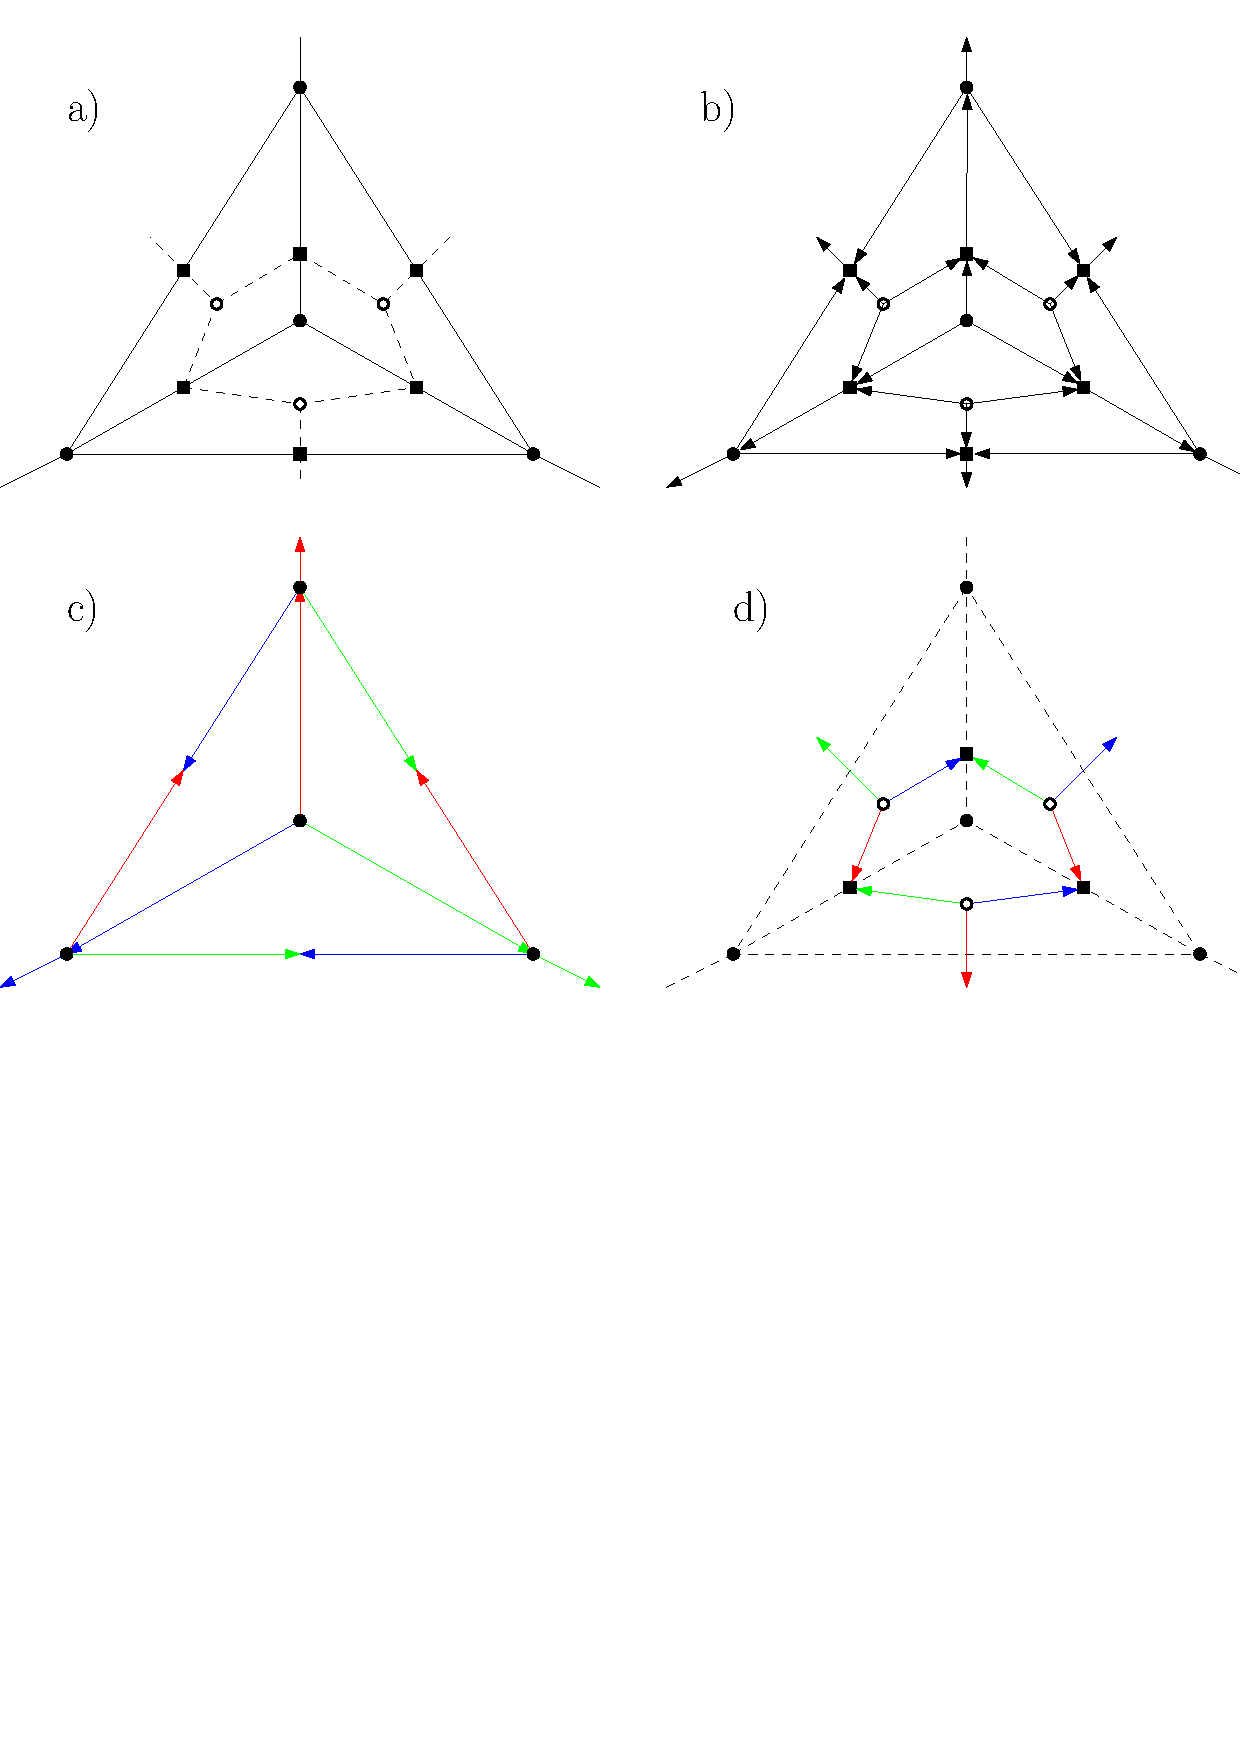
\includegraphics[width=0.8\textwidth]{alpha_ex.pdf}
  \caption{a) Der Primal-Duale Graph $K_4+K_4^*$. b) Mit einer $\alpha_s$-Orientiertung und c) den zugehörigen Schnyder Woods auf $K_4$ d) und $K^*_4$. }
  \label{alpha_ex}
\end{figure}

\begin{theorem}\label{alpha_bij}
Sei $G$ ein ebener Graph mit Aufhängungen $\{a_1,a_2,a_3\}$, dann stehen die folgenden Strukturen in Bijektion:
\begin{itemize}
\item [A1] Die Schnyder Woods auf $G$.
\item [A2] Die Schnyder Woods auf dem (schwachen) dualen Graphen $G^*$.
\item [A3] Die $\alpha_{s}$-Orientierungen des Abschlusses von $G+G^*$ mit $\alpha_s(v) = \alpha_s(f) = 3$ für jeden Knoten-Knoten $v$ und Gebiets-Knoten $f$,  $\alpha_s(e) = 1$ für jeden Kanten-Knoten $e$ und  $\alpha_s(f_\infty) = 0$.
\end{itemize}
\end{theorem}

Wir erklären kurz die erhaltene Bijektion von A1 und A2 zu A3. Angenommen wir haben ein Paar in Bijektion stehender Schnyder Woods $\sigma,\sigma^*$ auf $G$ und $G^*$. Die von $\sigma$ und $\sigma^*$ induzierte Orientierung der Kanten von $G+G^*$ ist eine $\alpha_s$-Orientierung. 

Angenommen wir haben eine $\alpha_s$-Orientierung auf dem Abschluss von $G+G^*$. Sie induziert die Orientierung der Kanten der resultierenden Schnyder Woods $\sigma$ und $\sigma^*$. Wir müssen jedoch noch die Label bestimmen. Dies erfolgt mit Hilfe der Gerader Pfad Regel. 

\begin{description}
\item[Gerader Pfad Regel:] Beginnen wir auf einer beliebigen Kante von $G+G^*$. Wenn wir einen Kanten-Knoten $e$ betreten, dann verlassen wir diesen auf der gegenüberliegenden Seite (wir folgen der zugrunde liegenden Kante in $G$ bzw. $G^*$). Wenn wir einen Knoten-Knoten oder Gebiets-Knoten $v$ betreten und über eine Kante kommen die zu $v$ orientiert ist, dann laufen wir auf der gegenüberliegenden, von $v$ weg orientierten Kante, weiter\footnote{Es existieren genau drei von $v$ weg orientierte Kanten und wir wählen die von uns aus gesehen Mittlere.} (vergleiche Abbildung \ref{straight_path} a). Falls wir $v$ über eine von $v$ weg orientierte Kante betreten, dann hängt unsere Wahl der Auskante von der Orientierung am letzten Kanten-Knoten $e$\footnote{Wir betreten Kanten-Knoten nur über zu diesen hin orientierte Kanten.} ab. Falls dort die Auskante auf der rechten Seite liegt, wählen wir jetzt die rechte\footnote{Falls wir $v$ durch eine von $v$ weg orientierte Kante betreten, dann bleiben noch zwei andere übrig.} von $v$ weg orientierte Kante, sonst die linke (vergleiche Abbildung \ref{straight_path} b). Falls wir $a_\infty$ erreichten laufen wir nicht weiter. 
\end{description}

\begin{figure}
	\centering
	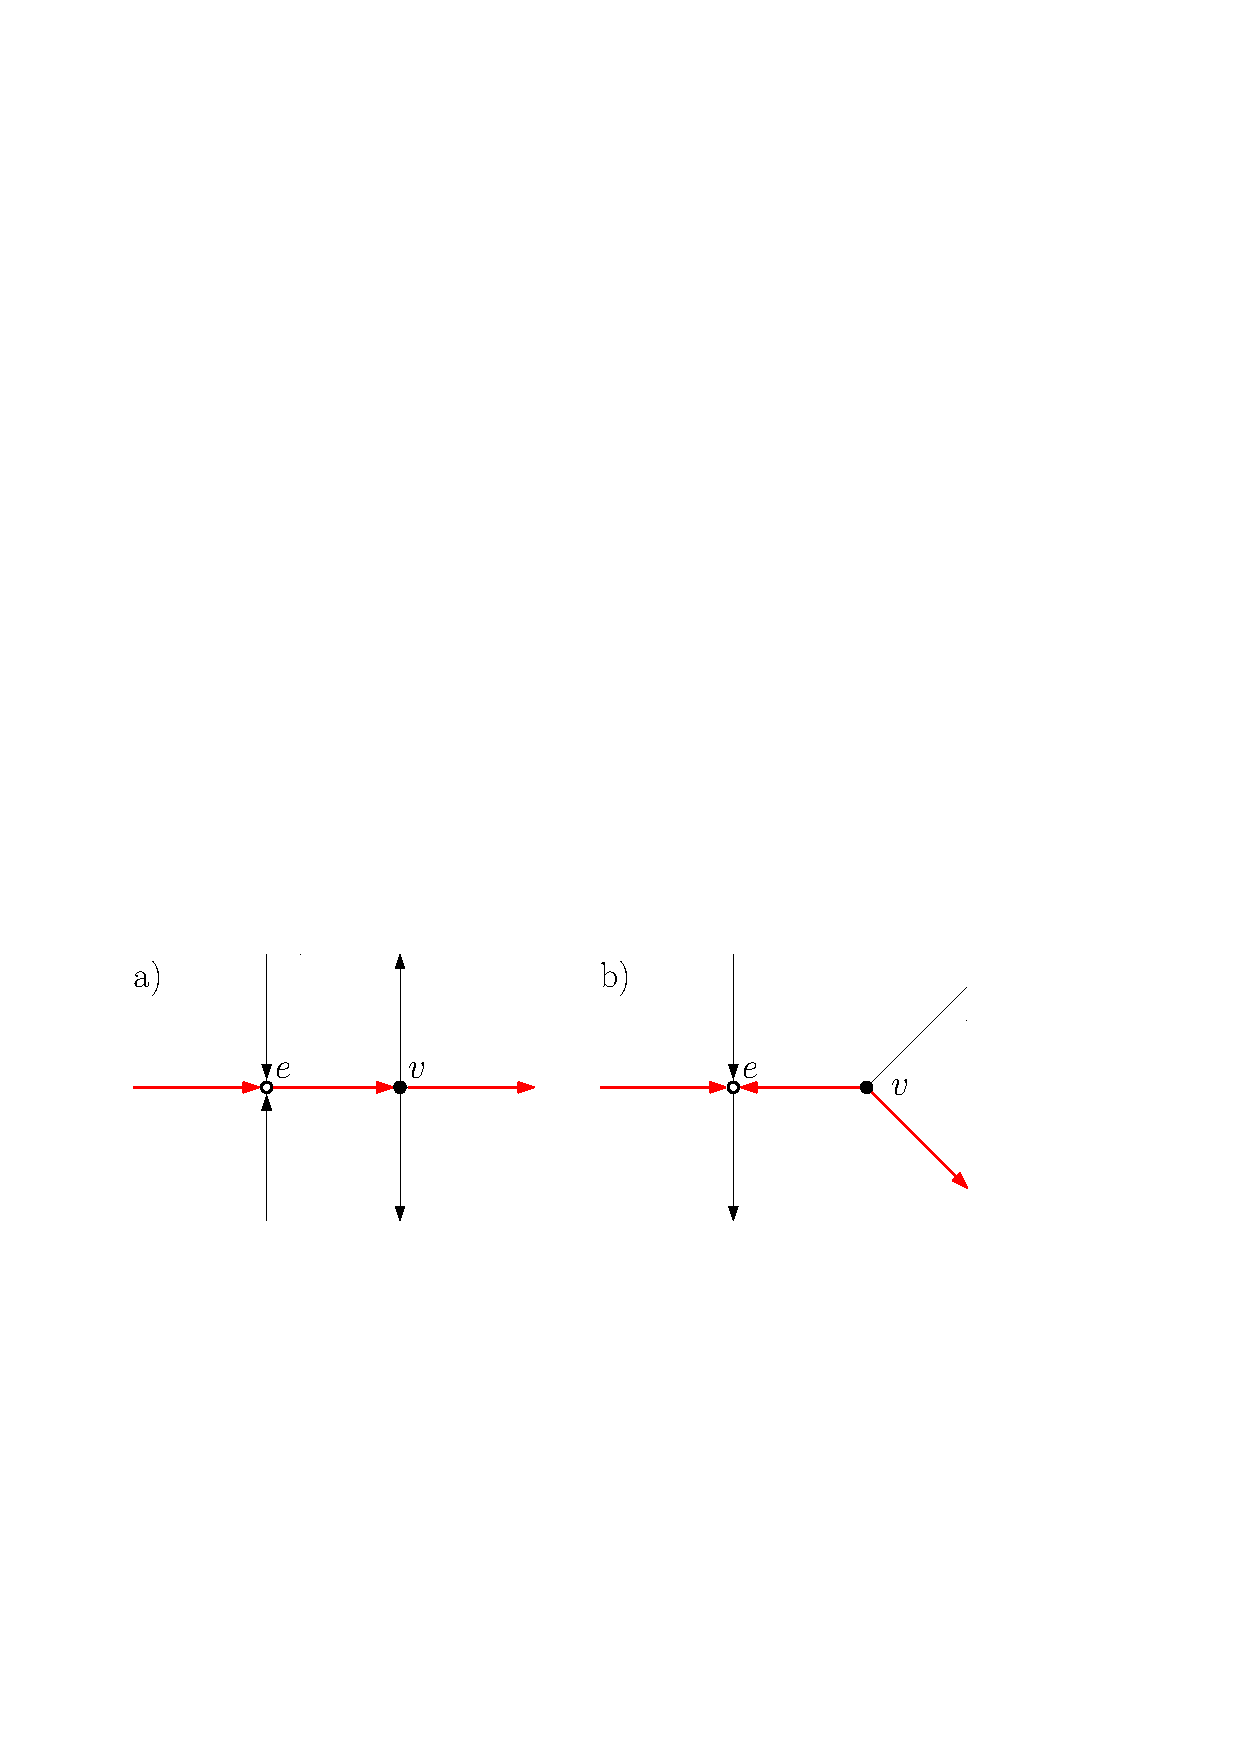
\includegraphics[width=0.7\textwidth]{straight_path.pdf}
  \caption{Die zwei Fälle der Gerader Pfad Regel beim Betreten eines Knoten $f$ aus $G$ oder $G^*$. In rot der gewählte und somit eingefärbte Pfad.}
  \label{straight_path}
\end{figure}

Betrachten wir einen Pfad nach der Regel, der mit einer gerichteten Kante $e \in G+G^*$ beginnt. Dann endet er in $a_\infty$ \cite[Lemma 15]{felsner01}. Der letzte passierte Knoten muss nun entweder eine der Aufhängungen von $G$ oder $G^*$ sein. Wir Färben den Pfad in der Farbe dieser Aufhängung. Die so erhaltene Orientierung und Färbung auf den Kanten von $G$ und $G^*$ entspricht zwei in Bijektion stehenden Schnyder Woods $\sigma$ und $\sigma^*$ \cite{felsner04}.

\section{Gerichtetes-Multi-Fluss-Problem}\label{dir_multi_flow}

Wir werden in Kapitel \ref{main_algo} einen gerichteten Graphen $\mathcal{N}$ auf Basis von $G$ konstruieren, sodass ein maximaler Fluss $\varphi$ einer SLTR von $G$ entspricht. Es gibt viele unterschiedliche Arten von Flussproblemen. So kann man zum Beispiel Graphen mit nur einem Paar von Quellen und Senken oder mit jeweils mehreren betrachten und die Kanten können gerichtet oder ungerichtet sein. Im Fall von mehreren Quellen und Senken werden diese normalerweise als Paare $s_i,t_i$ gehandhabt und es wird gefordert, dass insgesamt Fluss $\varphi_i$ mit Stärke $d_i \in \mathbb{R}_+$ von $s_i$ zu $t_i$ fließt. Als zusätzliche Einschränkung haben die Kanten $e$ Kapazitäten $c(e) \in \mathbb{R}_+$, die nicht überschritten werden dürfen. Für jede Kante muss also gelten $\varphi(e) \leq c(e)$. Wir werden uns in Kapitel \ref{main_algo} mit einem Fluss der folgenden Form befassen.

\begin{definition}[Gerichtetes-Multi-Fluss-Problem]\label{def_multi_flow}
Sei $\mathcal{N}=(V,E)$ ein gerichteter Graph, im Weiteren auch Netzwerk genannt, mit den Kapaziäten $c:E\mapsto\mathbb{R}_{+}$, Paaren von ausgezeichneten Knoten $\{(s_1,t_1), ... ,(s_n,t_n)\}\subset V \times V$ und positiven Bedarfen $\{d_1, ... ,d_n\} \in \mathbb{R}_+^n$. Dann bilden die Funktionen $\varphi_i: E \to \mathbb{R}_+^{|E|}$ einen zulässigen Fluss $\varphi=(\varphi_1, ... ,\varphi_n)$ auf $\mathcal{N}$, falls
\begin{itemize}
\item[M1] $\forall (u,v) \in E : \sum_{i=1}^{n}{\varphi_i(u,v)} \leq c(u,v) $
\item[M2] $ \forall u \neq s_i,t_i : \sum_{w \in V} \varphi_i(u,w) - \sum_{w \in V} \varphi_i(w,u) $
\item[M3] $ \forall s_i : \sum_{w \in V} \varphi_i(s_i,w) - \sum_{w \in V} \varphi_i(w,s_i) = d_i $
\item[M4] $ \forall t_i : \sum_{w \in V} \varphi_i(w,s_i) - \sum_{w \in V} \varphi_i(s_i,w) = d_i $
\end{itemize}
Mit $|\varphi_i|$ bezeichnen wir die Menge des Flusses von $s_i$ nach $t_i$.
\end{definition}

\begin{definition}
Wir nennen die Kantenmenge $S \subseteq \mathcal{N}_G(E)$ einen \textit{Schnitt} in $\mathcal{N}_G$, falls seine Entnahme alle Paare $\{s_i,t_i\}$ trennt. Die Kantenmenge $S$ ist ein \textit{minimaler Schnitt}, falls für alle anderen Schnitte $\tilde{S}$ gilt: $c(S) \leq c(\tilde{S})$.
\end{definition}

Es folgen zwei bekannte Resultate für den Fall $n=1$. Das erste Theorem stammt von Ford und Fulkerson \cite{ff09}.

\begin{theorem}[Max-Flow Min-Cut]
Der maximale zulässige Fluss auf einem Netzwerk $\mathcal{N}$ mit einer Quelle und Senke entspricht der Kapazität eines minimalen Schnittes.
\end{theorem}

Ein maximaler Fluss lässt sich zum Beispiel mit dem Edmonds-Karp-Algorithmus in polynomineller Zeit bestimmen \cite[Theorem 8.15]{korte12}. Ein direktes Resultat folgt nach Danzig und Fulkerson \cite{ff09}

\begin{theorem}[Ganzzahliger Fluss]\label{theo_int_flow}
Sei $\mathcal{N}$ ein Netzwerk mit einer Quelle und einer Senke und ganzzahligen Kapazitäten $c:E\mapsto\mathbb{N}$. Sei $\tilde{\varphi}$ ein nicht ganzzahliger Fluss auf $\mathcal{N}$. Dann existiert auch ein Fluss $\varphi$, mit $|\tilde{\varphi}| = |\varphi|$, sodass der Fluss $\varphi$ auf allen Kanten ganzzahlig ist.
\end{theorem}

Nach dem Max-Flow Min-Cut Theorem impliziert die Kapazität eines minimalen Schnittes im eindimensionalen Fall die Stärke eines maximalen Flusses. Für $n=2$ existieren für ungerichtete Graphen analoge Aussagen nach T. Chiang Hu \cite{hu}. Für diese Arbeit wäre im Folgenden jedoch der Fall $n=2$ für gerichtete Graphen interessant. Es existieren jedoch keine analogen Aussagen zum Max-Flow Min-Cut Theorem, welche für Gerichtete-Multi-Fluss-Probleme mit mindestens zwei Quellen und Senken aussagekräftig wären, sondern nur Schranken und Annäherungen \cite{leighton99}.

Im eindimensionalen Fall mit ganzzahligen Kapazitäten $c:E\mapsto\mathbb{N}$ impliziert die Existenz eines zulässigen Flusses nach Theorem \ref{theo_int_flow} die Existenz einer ganzzahligen Lösung, sowohl für gerichtete als auch für ungerichtete Graphen. Die Unterscheidung zwischen ganzzahligen und nicht ganzzahligen Flüssen ist relevant, da das Entscheidungsproblem, ob ein solcher Fluss existiert, im mehrdimensionalen Fall in unterschiedlichen Komplexitätsklassen liegt. Die Berechnung eines nicht (zwangsläufig) ganzzahligen zulässigen Flusses $\varphi$ auf $\mathcal{N}$ ist für den ein- und mehrdimensionalen Fall über eine LP-Formulierung in polynomieller Zeit möglich \cite[Theorem 4.18]{korte12}. Für ganzzahlige Lösungen gilt dies selbst in einfachen Fällen im Allgemeinen nicht und somit kann auch keine analoge Formulierung zu Theorem \ref{theo_int_flow} existieren.

\begin{theorem}[\cite{even75}]\label{np_hard}
Die Berechnung einer ganzzahligen Lösung eines Gerichtetes-Multi-Fluss-Problems auf einem Netzwerk $\mathcal{N}$ mit zwei Paaren von Quellen und Senken $\{(s_1,t_1),(s_2,t_2)\}$ und Kapazitäten $c:E\mapsto\mathbb{N}$ ist sogar dann NP-schwer, wenn $\mathcal{N}$ keine gerichteten Zykel enthält.
\end{theorem}

NP-schwere Entscheidungsprobleme lassen sich nicht in polynomieller Zeit lösen. Somit existiert kein im Allgemeinen gültiger deterministischer polynomieller Algorithmus zur Berechnung eines zulässigen ganzzahligen Flusses für ein Gerichtetes-Multi-Fluss-Problem für den Fall $n\geq2$.



\chapter{Hauptteil}

Sei $G$ ein planer intern 3-zusammenhängender Graph mit Aufhängungen $\{a_1,a_2,a_3\}$. Nehmen wir für einen Moment an, dass wir schon ein SLTR für $G$ gefunden haben, dann hat jeder Knoten $v$ in maximal einen inzidenten Gebiet $f$ einen falchen Winkel, mit $(v,f)$ bezeichnet, und liegt auf einer Geraden. Jedes Gebiet $f$ hat genau drei Ecken, also $deg(f)-3$ flache Winkel. Dies liefert im Umkehrschluss eine notwendige Bedingung für die Existent einer SLTR, indem wir die Knoten den Gebieten zuordnen.

\begin{definition}[FAA]
Sei $G=(V,E,F)$ ein planer Graph, dann ist eine Flache Winkel Zuordnung, im weiteren (nach dem englischen \textit{flat angle assignment}) mit FAA bezeichnet, ein Matching zwischen Knoten und Gebieten, sodass:
\begin{itemize}
\item [A1] Jedem Gebiet $f$ sind genau $deg(f)-3$ Knoten zugeordnet.
\item [A2] Jeder Knoten $v$ ist höchstens einem Gebiet zugeordnet.
\end{itemize}
Für den Fall das wir einen Graph mit Aufhängungen betrachten, dann fordern wir zusätzlich:
\begin{itemize}
\item [A3] Die inzidenten Knoten am äusseren Gebiet, die keine Aufhängungen sind, müssen dem äusseren Gebiet zugeordnet werden.
\end{itemize}
\end{definition}

%% Bild FAA mit und ohne SLTR!!

Ein planer Graph kann also nur dann eine SLTR besitzen, falls mindestens ein FAA existiert, jedoch liefert nicht jedes FAA sofort ein SLTR. Ein FAA, dass zu einer SLTR korrespondiert, wenn also die zugeordneten Winkel des FAA genau die flachen Winkel der SLTR sind, nennen wir von nun an \texit{Gutes-FAA} oder kurz \textit{GFAA}. Unser Ziel wird es sein solche Guten-FAA, und somit auch SLTRs, zu finden.

\section{Harmonische Funktionen}


\section{Ecken kompatible Paare}
\chapter{Algorithmen zur Erkennung von SLTRs}\label{main_algo}

Im vorherigen Kapitel wurden Kriterien für die Existenz einer SLTR für $G$ erarbeitet. Diese liefern allerdings nicht sofort einen Algorithmus, weder zur Frage nach der Existenz, noch für das Erlangen einer spezifischen SLTR. Dieses Kapitel wird sich diesem Thema zuwenden und einen von Aerts und Felsner in \cite{af15} erarbeiteten Algorithmus erläutern und analysieren.

\section{SLTRs via Zwei-Fluss}

Das Ziel ist es, für einen gegebenen ebenen intern-3-zusammenhängenden Graphen $G$ mit Aufhängungen $a_1,a_2,a_3$, sowohl einen Schnyder Wood als auch ein FAA jeweils als Lösung eines Fluss-Problems mit einer Quelle und Senke zu erhalten. Diese beiden werden dann in einem Zwei-Fluss-Problem kombiniert, sodass eine zulässige ganzzahlige Lösung ein Ecken-Kompatibles-Paar kodiert und somit eine SLTR resultiert. Wir beschäftigen uns also mit Multi-Fluss-Problemen auf gerichteten Graphen, die wir in Definition \ref{def_multi_flow} eingeführt haben.

\subsection{Schnyder-Wood-Fluss}

Um einen Schnyder Wood als Fluss-Problem zu kodieren, kann man die in Abschnitt \ref{alpha_orientations} eingeführten $\alpha_s$-Orientierungen auf dem Abschluss von $G+G^*$ nutzen. Fusy zeigt in \cite{fusy07} im Zuge der Untersuchung spezifischer $\alpha$-Funktionen, dass sich $\alpha_s$-Orientierungen von $G+G^*$ in linearer Zeit berechnen lassen, sodass wir auch einen Schnyder Wood auf $G$ in linearer Zeit erhalten.\\

Machen wir uns also an die Konstruktion eines Netzwerks $\mathcal{N}_S$ mit einer Quelle und Senke, sodass eine zulässige Lösung $\varphi_S$ einer $\alpha_s-Orientierung$ von $\tilde{G}$ entspricht, und somit auch einen Schnyder Wald auf $G$ liefert. Besonderes Augenmerk ist hier auf die Möglichkeit einer späteren Kombination mit einem FAA Fluss gelegt, um ein Kombiniertes Netzwerk zu erstellen, und nicht unbedingt auf Effizienz.\

Wie oben schon erwähnt ist $\tilde{G}$ bipartit, Kanten-Knoten haben Grad 4, Knoten-Knoten Grad $deg(v)$ und Gebiets-Knoten Grad $|f|$. Für eine $\alpha_s$-Orientierung muss jeder Kanten-Knoten Ausgrad 1, jeder Knoten-Knoten Eingrad $deg(v)-3$ und jeder Gebiets-Knoten Eingrad $|f|-3$ haben. Die Kanten-Knoten am äusseren Gebiet sind in $\tilde{G}$ immer nach aussen orientiert. Somit müssen wir nur die inneren Kanten-Kanten $E_{in}$ betrachten. \

\begin{figure}[h]
	\centering
  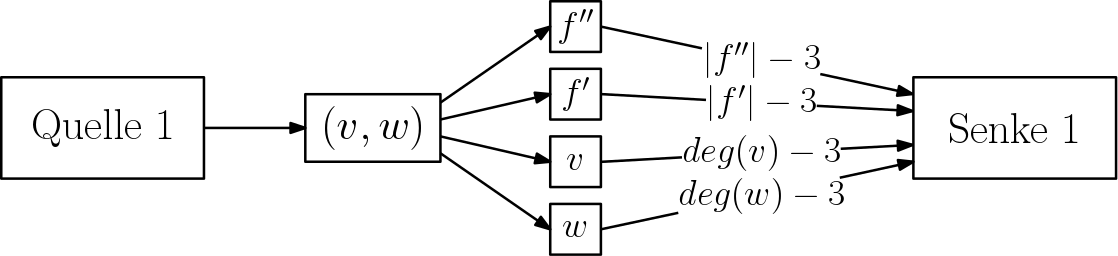
\includegraphics[width=0.9\textwidth]{schnyder_flow.png}
  \caption{Der Schnyder Wood Fluss durch eine innere Kante $(v,w)$.}
  \label{schnyder_flow}
\end{figure}

Sei $\mathcal{N}_S$ ein Netzwerk mit jeweils einer Quelle $s$ und Senke $t$, Kanten von der Quelle zu jedem $e \in E_{in}$ mit Kapazität 1, Kanten von den Kanten-Knoten $e$ zu inzidenten Knoten-Knoten $v$ und (inneren) Gebiets-Knoten $f \in F_{in}$ in $G$ ebenfalls mit Kapazität 1, Kanten von $f \in F_{in}$ zur Senke mit Kapazitäten $|f|-3$, Kanten von den (inneren) Knoten-Knoten $v \in V_{in} = V \setminus \{a_1,a_2,a_3\}$ zur Senke mit Kapazitäten $deg(v)-3$ und Kanten von den Aufhängungen $a_i$ zur Senke mit Kapazitäten $deg(a_i)-2$. Die letzte Kapazität resultiert aus dem Fakt, dass die Halbkante in $G+G^*$ von $a_i$ aus immer nach aussen orientiert ist und wir somit nur noch zwei andere Kanten nach aussen orientieren müssen.

Der Bedarf des Netzwerkes entspricht der Anzahl der inneren Kanten von $G$. Sei nun $\varphi_S$ eine zulässige ganzzahlige Lösung, dann hat jeder Kanten-Knoten $e$ Ausgrad 1. Der Fluss $\varphi_S$ entlang einer Auskante von $e \in E_{in}$ in $\mathcal{N}_S$ entspricht dann genau der hin zu $e$ orientierten Kante einer $\alpha_{s}$-Orientierung auf $G+G^*$. Die Knoten-Knoten und Gebiets-Knoten haben $deg(v)-3$ bzw. $|f|-3$ von $\varphi_S$ genutzte Auskanten und somit entspricht hier eine leere Kante in $\mathcal{N}_S$ einer von $v$ bzw. $f$ weg orientierten Kante bezüglich $\alpha_{s}$. Ein zulässiger ganzzahliger Fluss $\varphi_S$ kodiert also eine $\alpha_s$-Orientierung auf $G+G^*$. Somit existiert genau dann ein Schnyder Wald auf $G$, wenn eine ganzzahlige Lösung $\varphi_S$ für $\mathcal{N}_S$ existiert.

\subsection{FAA-Fluss}\label{faa-flow}

Um ein FAA für einen planaren Graphen $G$ zu erhalten, müssen wir jedem Gebiet $f \in F$ genau drei Ecken und $|f|-3$ flache Winkel zuordnen und jeder Knoten darf maximal einem Gebiet zugeordnet werden, also in diesem flach sein. Falls eine Einbettung und die Aufhängungen $\{a_1,a_2,a_3\}$ gegeben sind, müssen wir jedem inneren Gebiet $f \in F_{in}$ drei Ecken und $|f|-3$ flache Winkel zuweisen und jeder innere Knoten $v \in V_{in}$ darf maximal einem Gebiet zugeordnet werden. Wir konstruieren ein Netzwerk für den zweiten Fall, das sich leicht verallgemeinern lässt.\

Sei also wieder $\mathcal{N}_F$ ein Netzwerk mit einer Quelle und Senke, einem Knoten für jeden inneren Winkel $(f,v)$, mit $v\in V$ und $f \in F_{in}$, Knoten für alle inneren Gebiete $f$ und alle inneren Knoten $v$. Von der Quelle existiert eine Kante mit Kapazität 1 zu jedem inneren Winkel $(f,v)$, von jedem inneren Winkel $(f,v)$ jeweils eine Kante zu $f$ und zu $v$ mit Kapazität 1, von jedem inneren Gebiet $f$ eine Kante mit Kapazität 3 zur Senke und zuletzt noch eine Kante von jedem inneren Knoten $v$ zur Senke mit Kapazität 1. Der Bedarf des Netzwerks ist $\sum_{f \in F_{in}}{|f|}$ und entspricht der Anzahl der inneren Winkel von $G$. 

\begin{figure}[h]
	\centering
  
\includegraphics[width=0.8\textwidth]{faa_flow.png}
  \caption{Der FAA-Fluss durch einen Winkel $(f,v)$.}
  \label{faa_flow}
\end{figure}


Sei $\varphi_F$ ein zulässiger ganzzahliger Fluss, dann entspricht Fluss auf einer Kante $((f,v),f)$ einer Ecke (eines möglichen GFAAs) von $f$ und Fluss auf $((f,v),u)$ der Zuweisung eines Knoten zu $f$, also einem flachen Winkel in einem GFAA. Zur Vereinfachung sprechen wir im Weitern auch von Ecken- respektive Zuweisungs-Fluss. Somit wird jeder innere Winkel entweder dem Gebiet zugewiesen oder als Ecke ausgezeichnet und es kann nur jeweils ein Winkel an jedem inneren Knoten zugewiesen werden. $\varphi_F$ respektiert also die Bedingungen aus Definition \ref{def_faa} und es existieren nur dann FAAs auf $G$, wenn mindestens eine ganzzahlige Lösung für $\mathcal{N}_F$ existiert. Eine spezifische Lösung $\varphi_F$ entspricht genau einem FAA auf $G$.

\begin{remark}

Das oben konstruierte Netzwerk zur Bestimmung von FAAs lässt sich auch als Zwei-Fluss Problem konstruieren, wenn wir für Ecken- und Zuweisungs-Fluss getrennte Quellen und Senken einführen. Der Bedarf des Ecken-Flusses ist dann $3|F_{in}|$ und der Bedarf des Zuweisung-Flusses $\sum_{f \in F_{in}}{|f|-3}$.

\begin{figure}[h]
	\centering
  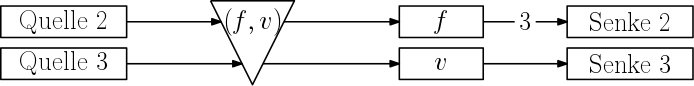
\includegraphics[width=0.8\textwidth]{faa_2_flow.png}
\end{figure}

Eine zulässige ganzzahlige Lösung $\varphi_F = (\varphi_{F_2},\varphi_{F_3})$ entspricht dann wieder einem FAA auf $G$, da aus der Ganzzahligkeit folgt, dass ein Winkel entweder von $\varphi_{F_2}$ oder $\varphi_{F_3}$ genutzt wird und somit eine Definition \ref{def_faa} respektierende Beschriftung der Winkel vorliegt.

\end{remark}




\subsection{Ein Zwei-Fluss Netzwerk zur Erkennung von SLTRs}

Im Verlauf des Kapitels haben wir nun sowohl für Schnyder Woods als auch für FAAs ein Netzwerk betrachtet, für das eine ganzzahlige Lösung einen Schnyder Wood bzw. ein FAA für einen planen Graphen $G$ liefert. Wir wollen jetzt eine Kombination aus beiden erstellen die ein Ecken kompatibles Paar $(\sigma,\phi)$ aus einem Schnyder Labeling $\sigma$ und einem FAA $\phi$  kodiert.\

Es folgt die Konstruktion eines Netzwerkes, wir bezeichnen es mit $\mathcal{N}_G$, welches diesen Wunsch erfüllt. Ein ganzzahliger Fluss $\varphi$ kodiert dann ein Ecken kompatibles Paar und impliziert somit nach Theorem \ref{theo_ccc} eine SLTR für $G$. Es handelt sich hierbei um ein 2-Fluss-Netzwerk.

Wie oben in Abschnitt \ref{faa-flow} erwähnt lässt sich ein FAA auch mit einem Zwei-Fluss kodieren und wir können Ecken- und Zuweisungs-Fluss mit den passenden Bedarfen getrennt betrachten. Wir müssen jetzt diese drei Flüsse, also Schnyder-, Ecken- und Zuweisungs-Fluss in einem Netzwerk kombinieren. In \cite{af15} ergeben Schnyder- und Ecken-Fluss zusammen Fluss von Typ 1 und der Zuweisungs-Fluss Typ 2. Wir wollen hier analog ein Netzwerk konstruieren in dem wir FAA und Schnyder-Wood Fluss nicht trennen. Der Verständlichkeit wegen werden wir Pfade, die in einer Lösung von einem der drei Flussarten genutzt werden, \textit{Schnyder-Pfad, Ecken-Pfad} und \textit{Zuweisungs-Pfad} nennen.\\

Bei der Kombination der beiden oben konstruierten Netzwerke $\mathcal{N}_S$ und $\mathcal{N}_F$ zu $\mathcal{N}_G$ müssen die Ecken Kompatibilität von Schnyder Labeling und FAA gewährleistet werden. K1 zu erfüllen, also die Nutzung der gleichen Aufhängungen von $\sigma$ und $\phi$, ist kein Problem. Allerdings müssen wir für die zweite Bedingung das Netzwerk etwas komplizierter machen. Betrachten wir als Basis $\mathcal{N}_S \cup \mathcal{N}_F$ und fürs erste nur das Teilnetzwerk um ein inneres Gebiet $f$, dann sehen wir, dass $f$ in $\mathcal{N}_S$ $|f|-3$ Schnyder-Fluss aufnimmt, aber $|f|$ Einkanten in $\mathcal{N}_S$ hat. Wir können die drei leeren Kanten für den Ecken-Fluss aus $\mathcal{N}_F$ nutzen. Um K2 zu erfüllen, müssen gewährleisten, dass jede Ecke im Schnyder Labeling ein anderes Label hat. Betrachten wir also die von $\varphi_S$ induzierte $\alpha_s$-Orientierung auf dem Abschluss von $G+G^*$. Nach Theorem \ref{alpa_bij} erhalten wir in Bijektion stehende Schnyder Labelings auf $G$ und $G^*$.

\begin{figure}[h]
	\centering
  	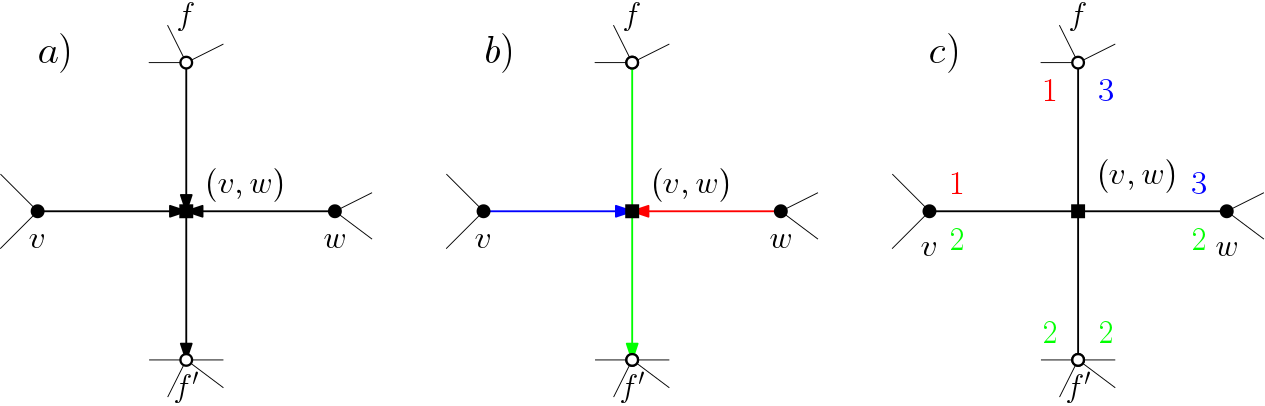
\includegraphics[width=0.9\textwidth]{alpha_bij.png}
  	\caption{a) Eine $\alpha_s$-Orientierung um eine innere Kante von $G$. b) Teile der korrespondierenden Schnyder Woods auf $G$ und $G^*$. c) Die induzierten Label, die für $G$ und $G^*$ gleich sind.}
	\label{alpha_bij}
\end{figure}

Für diese gilt, wie in Abbildung \ref{alpha_bij} skizziert, dass das Label der Ecke eines Gebietes in $G$ und das ihr in $G+G^*$ gegenüberliegenden Label der Ecke eines Gebiets um einen Knoten in $G^*$ gleich sind. Für eine zu $v$ in $G^*$ hin orientierte Kante folgt aus der Bijektion zwischen Schnyder Labelings und Schnyder Woods aus Abschnitt \ref{sw}, dass die Label links und rechts am Ende dieser Kante gleich sind. Somit sind auch die Label in $G$ gleich und wir können die folgende Eigenschaft festhalten.
\begin{itemize}
\item [A1] Die Label, des von $\alpha_s$ induzierten Schnyder Wood auf $G$, sind zwischen zwei aufeinander folgenden zu $f$ orientierten Kanten gleich.
\end{itemize}
Da es genau drei zu $f$ orientierte Kanten gibt müssen wir also dafür sorgen, dass für jedes Paar dieser Kanten eine Ecke zwischen ihnen liegt, da so die drei Ecken unterschiedliche Label haben und wir K2 erfüllen. Um dies zu erlangen implementieren wir eine zyklische Struktur um jedes innere Gebiet, wie in Abbildung \ref{combinded_face_sketch} skizziert.\\

\begin{figure}[h]
	\centering
  	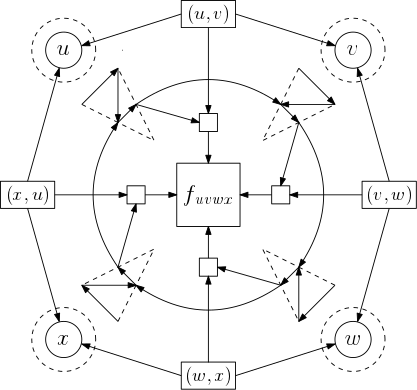
\includegraphics[width=0.9\textwidth]{combined_face_sketch.png}
  	\caption{Eine Skizze des kombinierten Netzwerkes auf einem inneren Gebiet mit $|f| = 4$. Beispielhaft sind Schnyder-Fluss (rot), Ecken-Fluss (blau) und Zuweisungs-Fluss (grün) eingezeichnet. }
	\label{combined_face_sketch}
\end{figure}

Betrachten wir zuerst den Schnyder-Fluss. Dieser wird Fluss von Typ 1, also von Quelle 1 zu Senke 1 sein. Für einen Schnyder-Pfad der durch einen Knoten $v$ führt hat sich nichts geändert. Der in der Skizze eingezeichnete Schnyder-Pfad der durch $f$ führt passiert davor einen extra Knoten, wir nennen ihn \textit{kleines Quadrat} der gewährleisten soll, dass von Seite des Gebietes aus entweder ein Schnyder-Pfad oder ein Ecken-Pfad in $f$ mündet. Zuletzt fügen wir wie oben von jedem inneren Gebiet eine Kante mit Kapazität $|f|-3$ zu Senke 1 ein. Somit kodiert hier eine ganzzahlige Lösung weiterhin einen Schnyder Wood auf $G$.\

Kommen wir nun zum FAA-Fluss, also Fluss von Typ 2. Von Quelle 2 geht genau wie in Abbildung \ref{faa_flow} eine Kante zu jedem inneren Winkel $(f,v)$. Ein Zuweisungs-Pfad verlässt diesen Winkel über einen zusätzlich zu $v$ eingefügten Dummy-Knoten $v^*$. Von jedem $v^*$ geht eine Kante mit Kapazität 1 zu einer Dummy-Senke und von dieser eine Kante mit Kapazität $\sum_{f \in F_{in}} |f|-3$ zu Senke 2, wie in Abbildung \ref{dummy_sink} illustriert.

Die Dummy-Knoten sorgen dafür, dass jeder Knoten im FAA nur einmal zugewiesen werden kann, ohne in Konflikt mit dem Schnyder-Fluss zu kommen. Die eingeschobene Dummy-Senke beschränkt die Anzahl der zugewiesenen Knoten, genau wie im zuvor konstruierten FAA-Fluss, auf $\sum_{f \in F_{in}} |f|-3$.

\begin{figure}[h]
	\centering
  	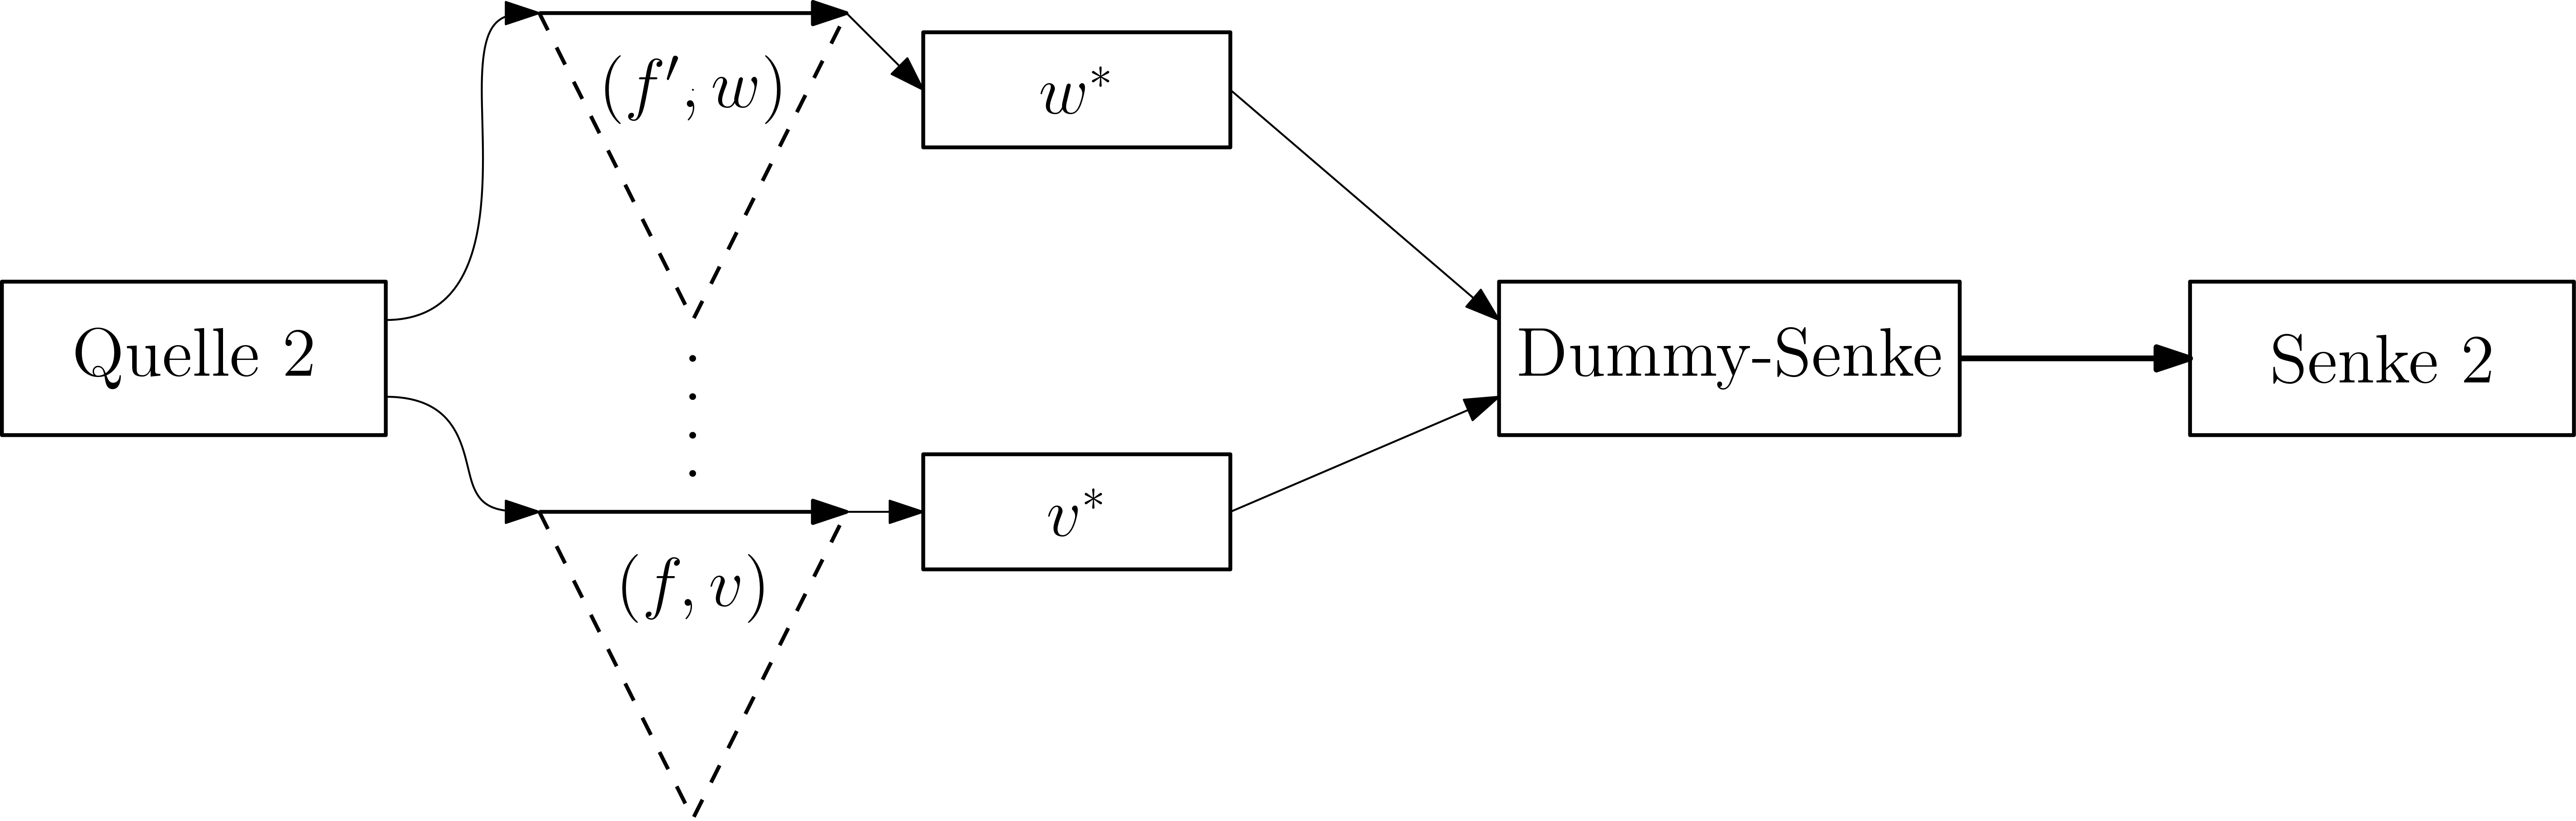
\includegraphics[width=0.7\textwidth]{dummy_sink.png}
  	\caption{Der Zuweisungsfluss durch die Winkel, Dummy-Knoten und die zusätzliche Kante vor Senke 2. Die Kante rechts hat Kapazität $\sum_{f \in F_{in}} |f|-3$ und alle anderen Kapazität 1.}
	\label{dummy_sink}
\end{figure}

Es bleibt der Ecken-Fluss. Hier betritt der Pfad das Gebiet $f$ wieder durch einen Winkel und muss es über ein ungenutztes kleines Quadrat verlassen. Die zweite und dritte Kante in jedem Winkeldreieck gewährleisten, dass nicht immer das nächste kleine Quadrat genutzt werden muss. Falls dies von Schnyder-Fluss besetzt ist und der nächste Winkel zugewiesen wird, kann ein Ecken-Pfad den nächsten Winkel passieren. Weiterhin sorgt die erste Kante, die von sowohl Schnyder-, als auch Winkel-Pfaden genutzt werden kann, für eine eindeutige Beschriftung (als Ecke oder nicht) im Falle einer ganzzahligen Lösung. Wie oben existieren auch hier Kanten von jedem inneren Gebiet zu Senke 2 mit Kapazität drei.\\

Betrachten wir die Bedarfe der beiden Flüsse von Typ 1 und Typ 2, $\varphi_1$ bzw. $\varphi_2$. Beide entsprechen jeweils den Bedarfen der oben konstruierten $\mathcal{N}_S$ und $\mathcal{N}_F$, da mit den gleichen Argumenten wie oben, ein Schnyder Wood und ein FAA kodiert werden können. Jedes Gebiet benötigt genau drei Ecken und $|f|-3$ zugewiesene Knoten und je ein Schnyder-Pfad führt durch jede innere Kante, $|E_{in}|$. Hier seien wieder $E_{in}$ die inneren Kanten und $F_{in}$ die inneren Gebiete von $G$. Es gilt also:

\begin{itemize}
\item $d_1$ = Bedarf$(\varphi_1) = $ Bedarf$(\varphi_S) = |E_{in}|$
\item $d_2$ = Bedarf$(\varphi_2) = $ Bedarf$(\varphi_F) =  \sum_{f \in F_{in}}(|f|-3) + 3|F_{in}| = \sum_{f \in F_{in}} |f|$
\end{itemize}

Bevor wir in Theorem \ref{theo_algo} zeigen, dass eine ganzzahlige Lösung $\varphi=(\varphi_1,\varphi_2)$ auch wirklich ein Ecken kompatibles Paar kodiert, wollen wir noch ein Paar weitere Beobachtungen festhalten. Nehmen wir also an, wir haben eine ganzzahlige Lösung $\varphi$ gefunden, dann gilt für diese:
\begin{itemize}
\item [A2] Jede äussere Kante in einem Winkel-Dreieck ist ausgelastet, sie wird entweder von einem Ecken- oder Zuweisungspfad genutzt.
\item [A3] Jede Kante von einem kleinen Quadrat zu einem inneren Gebiet $f$ ist ausgelastet, sie wird entweder von einem Schnyder- oder Ecken-Pfad genutzt.
\item [A4] Ein inneres Gebiet $f$ mit $|f|=3$ kann nicht von Zuweisungs- bzw. Schnyder-Pfaden genutzt werden.
\end{itemize}

Wir wollen diese Beobachtungen kurz begründen. Für jede mögliche ganzzahlige Lösung $\varphi$ gilt $$|\varphi|=|\varphi_1|+|\varphi_2| = |E_{in}| + \sum_{f \in F_{in}} |f|.$$
Da es genau $\sum_{f \in F_{in}} |f|$ innere Winkel gibt und der FAA-Fluss $\mathcal{N}_G$ nur durch diese betreten kann ergibt sich A2. A3 wird aus Gleichung \ref{eq_sat} weiter unten folgen. Durch ein inneres Gebiet $f$ müssen drei Ecken-Pfade führen und im Fall $|f|=3$ führt dies zu A4, da kein Platz in den Winkeln für Zuweisungs-Pfade und keine freien kleinen Quadrate für Schnyder-Pfade existieren.

\begin{theorem}\label{theo_algo}
Sei $G$ ein intern-3-zusammenhängender Graph mit gegebenen Aufhängungen $\{a_1,a_2,a_3\}$, dann existiert eine SLTR von $G$, genau dann wenn ein ganzzahliger zulässiger Fluss $\varphi=(\varphi_1,\varphi_2)$ auf $\mathcal{N}_G$ existiert.
\end{theorem}

Fassen wir vor dem Beweis noch einmal das Netzwerk zusammen.

\begin{network}[SLTR]\label{net_sltr}
Bei $\mathcal{N}_G$ handelt es sich um ein gerichtetes Netzwerk, das auf Basis von $G$ erstellt wird, um eine SLTR von $G$ zu finden. Ein Ausschnitt um ein inneres Gebiet ist in Abbildung \ref{theo_algo} dargestellt.
	\begin{itemize}
	\item $\mathcal{N}_G$ hat zwei Quellen $s_1,s_2$ und zwei Senken $t_1,t_2$
	\item Knoten in $\mathcal{N}_s$ werden für jeden innere Kante $e \in E_{in}$, jedes innere Gebiet $f\in F_{in}$ und jeden Knoten $v \in V$ aus $G$ erzeugt.
	\item Es werden Knoten der folgenden Typen in $\mathcal{N}_S$ erzeugt:
		\begin{itemize}
		\item Knoten $e$ für jede innere Kante $e \in E_{in}$
		\item Knoten $v$ für jeden $v \in V$ und Dummy-Knoten $v^*$ für jeden $v \in V_{in}$
		\item Knoten für jedes innere Gebiet $f$.
		\item $|f|$ kleine Quadrate $q$ um jedes innere Gebiet $f$
		\item Vier Knoten $w_1,w_2,w_3,w_4$ für jedes innere Winkeldreieck
		\item Die Dummy-Senke $t_d$
		\end{itemize}
	\item Es werden gerichtete Kanten der folgenden Typen in $\mathcal{N}_G$ erzeugt:
		\begin{itemize}
		\item $(s_1,e)$ von Quelle 1 zu jeder inneren Kante mit $c\big(s,e\big) = 1$
		\item $(e,v_1),(e,v_2)$ von jeder inneren Kante zu den Endknoten mit $c\big(e,v\big) = 1$
		\item $(e,q)$ von inneren Kanten zu adjazenten kleinen Quadraten mit $c\big(e,q\big) = 1$
		\item $(q,f)$ von jeder kleinen Quadraten zu den inneren Gebieten mit $c\big(q,f\big) = 1$
		\item $(f,t_1)$ von den inneren Gebieten zur Senke 1 mit $c\big(f,t_1\big) = |f|-3$
		\item $(a_i,t_1)$ von den Aufhängungen zur Senke 1 mit $c\big(f,t\big) = \text{deg}(a_i)-2$
		\item $(v,t_1)$ von den restlichen Knoten zur Senke 1 mit $c\big(f,t\big) = \text{deg}(v)-3$		
		\item $(s_2,(f,v))$ von Quelle 2 zu jedem inneren Winkel mit $c\big(s_2,(f,v)\big) = 1$
		\item $(w_1,w_2),(w_2,w_3),(w_3,w_4)$ in jedem inneren Winkel mit $c\big(w_i,w_{i+1}\big) = 1$
		\item $(t_4,q)$ von inneren Winkeln zum nächsten kleinen Quadrat mit $c\big(t_4,q\big) = 1$
		\item $(t_4,t'_3)$ von inneren Winkeln zum nächsten inneren Winkel mit $c\big(t_4,t'_3\big) = 1$
		\item $((f,v),f)$ von inneren Winkeln zum Gebiet mit $c\big((f,v),f\big) = 1$
		\item $(t_2,v*)$ von jedem inneren Winkel zum Dummy-Knoten mit $c\big(t_2,v^*\big) = 1$
		\item $(v^*,t_d)$ von den Dummy-Knoten zur Dummy-Senke mit $c\big(f,t\big) = 1$
		\item $(t_d,t_2)$ von der Dummy-Senke zu Senke 2 mit $c\big(t_d,t_2\big) = \sum_{f \in F_{in}}|f|-3$
		\end{itemize}
	\item $\mathcal{N}_S$ hat Bedarfe $d_1=|E_{in}|$ und $d_2 = \sum_{f \in F_{in}}|f|$
	\item [$\Rightarrow$] Ein zulässiger ganzzahliger Fluss $\varphi = (\varphi_1,\varphi_2)$ existiert. $\Leftrightarrow$ Es existiert ein SLTR  auf $G$.
	\end{itemize}
\end{network}	

\begin{proof}[Beweis von Theorem \ref{theo_algo}]
Sei $G$ ein intern-3-zusammenhängender Graph mit Aufhängungen $\{a_1,a_2,a_3\}$ und $\varphi=(\varphi_1,\varphi_2)$ sei ein ganzzahliger machbarer Fluss auf $\mathcal{N}_G$. Im ersten Schritt extrahieren wir einen Schnyder-Wood $\sigma$ und ein FAA $\phi$, um dann zu zeigen, dass sie ein Ecken kompatibles Paar bilden. Für einen machbaren Fluss müssen die Bedarfe erfüllt werden. Es gilt somit $|\varphi_1| =  |E_{in}|$ und $|\varphi_2| = \sum_{f \in F_{in}} |f|$.
\begin{equation}\label{eq_sat}
\begin{split}
|\varphi_1| + |\varphi_2| & = \sum_{f \in F_{in}} (|f|-3) + 3|F_{in}| + |E_{in}|\\
		& = \sum_{f \in F_{in}} (|f|-3) + 2|E| -|V| - 1 + 2|F| - |f_{aus}|\\
		& = \sum_{f \in F_{in}} (|f|-3) + \sum_{v \in V} (\text{deg}(v)-3) + 2|V| + 2|F| - 1 - |f_{aus}|\\
		& = \sum_{f \in F_{in}} (|f|-3) + \sum_{v \in V} (\text{deg}(v)-3) + 2|E| + 3 - |f_{aus}|\\
		& = \underbrace{\sum_{f \in F_{in}}(|f|-3)  }_{\text{\parbox{8em}{Dummy-Senke zu Senke 2}}} + \underbrace{\sum_{v \in V} (\text{deg}(v)-3) +3 }_{\text{\parbox{10em}{Kapazität Senke 2 von den Knoten.}}} +\underbrace{\sum_{f \in F_{in}}(|f|-3) + 3|F_{in}|}_{\text{\parbox{12em}{Kanten von den Quadraten zu den inneren Gebieten}}}
\end{split}
\end{equation}

Die beiden Terme in der rechten unteren Klammer entsprechen den Kapazitäten von den inneren Gebieten zu Senke 1 und Senke 2. Somit sind alle Kanten zu den Senken ausgelastet. Die Kanten von den kleinen Quadraten zu den inneren Gebieten sind ebenfalls ausgelastet. Diese sind die einzigen Kanten in $\mathcal{N}_G$, die sowohl von $\varphi_1$ als auch $\varphi_2$ genutzt werden können. Kapazität eins und Ganzzahligkeit von $\varphi$ impliziert somit A3.\\

Beginnen wir mit $\varphi_1$ um einen Schnyder Wood, oder genauer eine $\alpha_s$-Orientierung, zu erhalten. $|\varphi_1| = |E_{in}|$, somit führt durch jede innere Kante ein Schnyder-Pfad und dieser gibt uns die nach aussen gerichtete Kante in $\alpha_s$. Es bleibt zu zeigen, dass für jedes innere Gebiet und jeden Knoten die Bedingungen aus Theorem \ref{alpha_bij} für eine $\alpha_s$ eingehalten werden. Da alle Kanten von den Knoten zu Senke 1 ausgelastet sind folgt, dass durch jeden inneren Knoten $v$ genau $\text{deg}(v)-3$ Schnyder-Pfade führen. Somit ergeben die leeren Einkanten von $v$ in $\mathcal{N}_G$ die drei Auskanten für $\alpha_s$. Für eine Aufhängung $a_i$ folgt analog, dass die beiden ungenutzten Einkanten, zusammen mit der Halbkante ins äußere Gebiet, die Bedingungen der $\alpha_s$-Orientierung erfüllen. Es bleibt zu zeigen, dass durch jedes innere Gebiet $|f|-3$ Schnyder-Pfade führen. Der restliche Schnyder-Fluss $|E_{in}| - \sum_{v \in V} (\text{deg}(v)-3)$ muss durch die inneren Gebiete führen und aus der ersten und letzten Zeile von Gleichung \ref{eq_sat} folgt $$|E_{in}| - \sum_{v \in V} (\text{deg}(v)-3) = \sum_{f \in F_{in}} (|f|-3).$$
Somit führen $|f|-3$ Schnyder-Pfade durch jedes innere Gebiet und wir können die $\alpha_s$-Orientierung vervollständigen und erhalten einen Schnyder Wood auf $G$.\\

Betrachten wir nun $\varphi_2$. Nach A4 sind alle äusseren Kanten in den Winkeln ausgelastet. Falls diese nun in jedem inneren Gebiet von drei Ecken-Pfaden und $|f|-3$ Zuweisungs-Pfaden genutzt werden, können wir ein FAA extrahieren. Da alle Kanten zu Senke 2 ausgelastet sind, führen $\sum_{f \in F_{in}} (|f|-3)$ Pfade durch die Dummy-Senke. Somit werden auch $\sum_{f \in F_{in}} (|f|-3)$ Knoten inneren Gebieten zugewiesen. Indem wir die Pfade zurückverfolgen und sehen aus welchem Gebiet der Zuweisungs-Pfad einen Dummy-Knoten betritt, können wir diese Informationen auslesen. Es bleibt zu zeigen, dass jedem Gebiet genau $|f|-3$ Knoten zugewiesen werden. Dies gilt, wenn durch jedes Gebiet drei Ecken-Pfade laufen und folgt somit, da die Kanten von den inneren Gebieten zu Senke 2 ausgelastet sind. Wir können also aus $\varphi_2$ ein FAA für $G$ extrahieren. \\

Nun müssen wir zeigen, dass $\sigma$ und $\phi$ ein Ecken kompatibles Paar ergeben. C1, dass beide die gleichen Aufhängungen nutzen folgt sofort aus der Konstruktion von $\mathcal{N}_G$. Es bleibt C2.\

Betrachten wir ein Teilnetzwerk (wie in Abbildung \ref{combined_face_sketch}) um ein inneres Gebiet $f$. Die drei Ecken-Pfade können keine der $|f|-3$ kleinen Quadrate nutzen die schon von Schnyder-Fluss okkupiert werden. Die drei übrigen kleinen Quadrate nennen wir \textit{verfügbar}. Ausgehend von $f$ folgen wir den Ecken-Pfaden rückwärts zu den verfügbaren kleinen Quadraten. Wenn wir das Quadrat verlassen gelangen wir zur dritten Kante eines Winkeldreiecks (entgegen dem Uhrzeigersinn). Nun verlassen wir das Gebiet entweder über diesen Winkel oder bewegen uns weiter (entgegen dem Uhrzeigersinn) zum nächsten Winkeldreieck. Doch wir werden zeigen, dass dies nur dann geschieht wenn das kleine Quadrat zwischen diesen nicht \textit{verfügbar} ist. Also betritt zwischen zwei \textit{verfügbaren} kleinen Quadraten ein Ecken-Pfad das Gebiet und die Winkel haben nach A1 unterschiedliche Label.

\begin{claim}\label{claim1}
Seien $Q_1,Q_2$ und $Q_3$, im Uhrzeigersinn, die drei verfügbaren kleinen Quadrate um ein inneres Gebiet $f$. Dann existiert ein Ecken-Pfad, welcher das Netzwerk über $Q_i$ verlässt. Dieser betritt es in einem Winkel zwischen, im Uhrzeigersinn, $Q_{i-1}$ und $Q_i$.
\end{claim}

Angenommen dies ist nicht der Fall und nehmen wir ohne Beschränkung der Allgemeinheit an, dass der Ecken-Pfad $P_e$ das Gebiet durch $Q_3$ verlässt. Der Winkel über den $P_e$ das Teilnetzwerk um das innere Gebiet betritt liegt also nicht zwischen $Q_2$ und $Q_3$. Angenommen er liegt zwischen $Q_1$ und $Q_2$. Betrachte das letzte Winkeldreck vor $Q_2$. Nach unserer Annahme ist die innere Kante dieses Dreiecks von $P_e$ ausgelastet. Somit kann kein Ecken-Fluss zu $Q_2$ gelangen und wir erhalten einen Widerspruch, da alle kleinen Quadrate entweder von Ecken- oder von Schnyder-Fluss genutzt werden müssen. Mit dem gleichen Argument kann $P_e$ das Teilnetzwerk nicht zwischen $Q_3$ und $Q_1$ betreten. Somit ist Behauptung \ref{claim1} wahr.

\begin{claim}
Alle Winkel zwischen zwei aufeinander folgenden verfügbaren kleinen Quadraten, haben die selben Label im Schnyder Labeling $\sigma$.
\end{claim}
Diese Behauptung folgt aus der in Abbildung \ref{alpha_bij} illustrierten Bijektion zwischen der $\alpha_S$ Orientierung und den Schnyder Labelings auf $G$ und $G^*$. Die Winkel links und rechts von einem kleinen Quadrat, dass von einem Schnyder-Pfad genutzt wird, haben das gleiche Label in $\sigma$, da diese den Einkanten in $\alpha_s$ entsprechen. Die Auskanten entsprechen den verfügbaren kleinen Quadraten, und hier ändern sich die Label.\\

Diese beiden Behauptungen zusammen zeigen, dass jede Ecke aus $\phi$ ein anderes Label in $\sigma$ hat. Somit handelt es sich um ein Ecken Kompatibles Paar $(\sigma,\phi)$.\\

Wir haben die Rückrichtung gezeigt. Nehmen wir also an, dass eine SLTR für $G$ existiert. Wir müssen nun einen zulässigen ganzzahligen Fluss $\varphi=(\varphi_1,\varphi_2)$ auf $\mathcal{N}_G$ konstruieren, der die SLTR kodiert. Nach Theorem \ref{theo_ccc} existiert ein Ecken kompatibles Paar $(\sigma,\phi)$ aus einem Schnyder Labeling $\sigma$ und einem FAA $\phi$, das zu diesem SLTR passt. Betrachte die zu $\sigma$ gehörige $\alpha_s$-Orientierung.

Wir beginnen mit einem leeren, wie oben konstruierten Netzwerk $\mathcal{N}_G$ und werden nun Schritt für Schritt einen zulässigen Fluss $\varphi$ konstruieren.

Zuerst fügen wir für jeden zugewiesenen Winkel einen Pfad von Quelle 2, über die äussere Kante des Winkeldreiecks, den zugehörigen Dummy-Knoten und die Dummy-Senke hin zu Senke 2 ein. Es kommen somit $\sum_{f \in F_{in}}|f|-3$ Einheiten Fluss hinzu und die Kante von der Dummy-Senke zu Senke 2 wird ausgelastet.

Als nächsten fügen wir den Fluss hinzu, der die $\alpha_s$-Orientierung kodiert. Zuerst von Quelle 1 zu jedem inneren Kanten-Knoten $e$, dann von den inneren Kanten entweder über ein kleines Quadrat in ein angrenzendes Gebiet oder zu einem benachbarten Knoten je nachdem, wohin die Auskante von $e$ in $\alpha_s$ zeigt. Zuletzt saturieren wir die Kanten von den inneren Knoten und inneren Gebieten zu Senke 1.

Zuletzt müssen wir den Ecken-Fluss einfügen. Ein Ecken-Pfad $P_e$ entspringt in Quelle 1, nutzt das zugehörige Winkeldreieck (diese sind noch frei) und verlässt das Gebiet über das im Uhrzeigersinn nächste verfügbare kleine Quadrat, wieder. 

Es sind alle Kanten hin zu den Senken ausgelastet. Ebenso kann man sehen, dass an keiner Kante die Kapazität überschritten wird. Somit haben wir einen zulässigen ganzzahligen Fluss kostruiert, der eine SLTR kodiert. Damit ist der Beweis abgeschlossen.

\end{proof}

\section{Nicht ganzzahlige Lösungen}

Dieses Kapitel wird sich mit der von Aerts und Felsner offen gelassenen Frage beschäftigen, ob die Erkennung von Graphen mit einer SLTR in $\mathcal{P}$ liegt. Wie in Kapitel \ref{pre} erwähnt, impliziert eine nicht ganzzahlige Lösung für ein Multi-Fluss-Problem auf einem gerichteten Graphen mit $n\geq 2$ Paaren von Quellen und Senken, im Allgemeinen nicht die Existenz einer ganzzahligen Lösung. Die Ergebnisse aus Kapitel \ref{the_program} lassen jedoch die Möglichkeit offen, dass das man für das betrachtete Netzwerk $\mathcal{N}_G$ die folgende Vermutung beweisen kann.

\begin{conjecture}\label{int_conj}
Sei $\tilde{\varphi}=(\tilde{\varphi_1},\tilde{\varphi_2})$ ein nicht ganzzahliger zulässiger Fluss auf $\mathcal{N}_G$, dann existiert auch ein ganzzahliger zulässiger Fluss $\varphi$ und wir können in polynomieller Zeit ein Gutes-FAA aus $\tilde{\varphi_2}$ extrahieren, ohne eine ganzzahlige Lösung zu berechnen.
\end{conjecture}

\begin{remark}
Wenn wir nicht darauf bestehen, dass unsere Lösung ganzzahlig ist, dann lässt sich eine Lösung nach TODO durch lineare Programmierung in polynomineller Zeit finden und das Entscheidungsproblem, ob ein Graph eine SLTR hat läge so in $\mathcal{P}$.
\end{remark}

Um die Argumentation einfacher zu gestalten, werden wir unser 2-Fluss Problem manchmal als 3-Fluss Problem, mit einer Lösung $\varphi=(\varphi_s,\varphi_e,\varphi_z)$, betrachten. Wir erstellen $\mathcal{N}^*_G$ wie zuvor $\mathcal{N}_G$, nur mit drei Quellen und Senken und weisen {Schnyder-,} Ecken-, und Zuweisungs-Fluss eigene Typen zu. Man kann leicht sehen, dass Theorem \ref{theo_algo} in angepasster Form hier ebenfalls gilt und ein zulässiger  Fluss $(\varphi_s,\varphi_z,\varphi_e)$ auf $\mathcal{N}_G^*$ genau dann existiert, wenn auch ein zulässiger Fluss $(\varphi_1,\varphi_2)$ auf $\mathcal{N}_G$ möglich ist. Die Hinrichtung ist klar. Nehmen wir an $(\varphi_1,\varphi_2)$ ist eine ganzzahlige Lösung. Nach Beobachtung A2 gilt, dass die äusseren Kanten eines Winkel-Dreiecks entweder von einem Ecken- oder einem Zuweisungs-Pfad genutzt werden. Diese Kanten sind zusammen mit den Kanten von Quelle 2 zu den Winkeldreiecken die einzigen in $\mathcal{N}_G$, die von beiden Flüssen genutzt werden. Wir können also $\varphi_2$ in $|\varphi_2|$ ganzzahlige Pfade aufteilen und jeden Pfad entweder $\varphi_e$ oder $\varphi_z$ zuweisen -- je nachdem ob er über die Dummy-Senke führt, oder nicht. Insbesondere folgt mit der gleichen Argumentation:

\begin{itemize}
\item [O1] Jede beliebige Kombination von $\varphi_s,\varphi_e$ und $\varphi_z$ zu zwei Flüssen und ein zu $\mathcal{N}_G$ analoges Netzwerk hat eine zulässige ganzzahlige Lösung genau dann, wenn eine Lösung für das 3-Fluss-Netzwerk existiert.
\end{itemize}

Betrachten wir zunächst den zweiten Teil von Vermutung \ref{int_conj}.

\begin{lemma}\label{lem_faa}
Sei $\tilde{\varphi}$ ein nicht ganzzahliger zulässiger Fluss auf $\mathcal{N}_G$ und sei $W$ die Menge der vom Zuweisungsfluss $\tilde{\varphi}_z$ genutzten inneren Winkel von $G$. Dann existiert eine Teilmenge $\phi\subseteq W$, sodass aus jedem Gebiet $f$ genau $|f|-3$ Winkel in $\phi$ enthalten sind und in der jeder Knoten $v$ höchstens einmal vorkommt. $\phi$ kodiert also ein FAA von $G$.
\end{lemma}

\begin{proof}
Wir betrachten das gerichtete Netzwerk $\mathcal{F}_z$ mit einer Quelle $s$ und Senke $t$, einem Beutel $B_f$ für jedes innere Gebiet $f$, einem Knoten $(f,v)$ für jeden inneren Winkel und einem Knoten für jeden Dummy-Knoten. Zuerst fügen Kanten mit Kapazität $|f|-3$ von der Quelle zu jedem Beutel ein. Dann folgen Kanten von den Beuteln $B_f$ zu den Winkeln von $f$, von den Winkeln $(f,v)$ zu den Dummy-Knoten $v^*$ und zuletzt eine Kante von jedem Dummy-Knoten zu Senke mit Kapazität 1, jeweils mit Kapazität 1. Der maximal mögliche $s$-$t$-Fluss in $\mathcal{F}_z$ ist $\sum_{f \in F_{in}}(|f|-3)$, da die Kanten zu den Beuteln einen Schnitt bilden und wir  aus $\tilde{\varphi}_z$ sofort eine zulässige nicht ganzzahlige Lösung $\tilde{\phi}$ für $\mathcal{F}_z$ konstruieren können. Nach Theorem \ref{theo_int_flow} existiert somit ein ganzzahliger Fluss $\phi$ auf $\mathcal{F}_z$, mit $|\phi| = |\tilde{\phi}| = |\tilde{\varphi}_z| = \sum_{f \in F_{in}}(|f|-3).$

\begin{figure}
	\centering
  	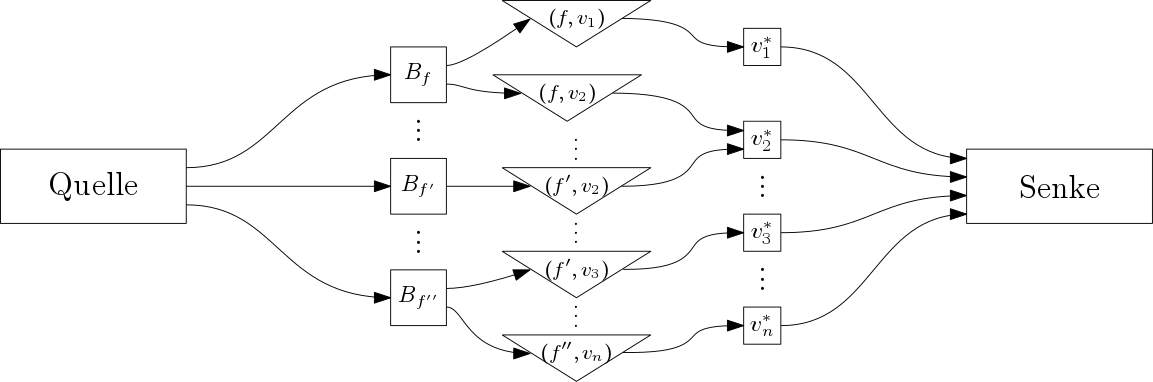
\includegraphics[width=0.7\textwidth]{lem_faa_choice.png}
  	\caption{Skizze des Netzwerkes $\mathcal{F}_z$. Die Kanten von der Quelle zu einem Beutel $B_f$ hat Kapazität $|f|-3$ und alle anderen haben Kapazität 1.}
\end{figure}

$\phi$ weißt nun jedem inneren Gebiet $f$ genau $|f|-3$ Winkel zu und jeder Knoten $v$ kann nur einmal zugewiesen werden. Wenn wir noch die per Konstruktion von $\mathcal{N}_G$ zugewiesenen Knoten am äusseren Gebiet hinzunehmen, dann kodiert $\phi$ ein FAA von $G$.
\end{proof}

\begin{remark}
Es ist uns nicht möglich mit beliebigen Winkeln aus $W$ zu beginnen und Schritt für Schritt für jedes Gebiet $|f|-3$ Winkel wählen, wie in Abbildung \ref{lem_faa_choice_ex} illustriert ist.
\end{remark}
\begin{figure}[h]
	\centering
  	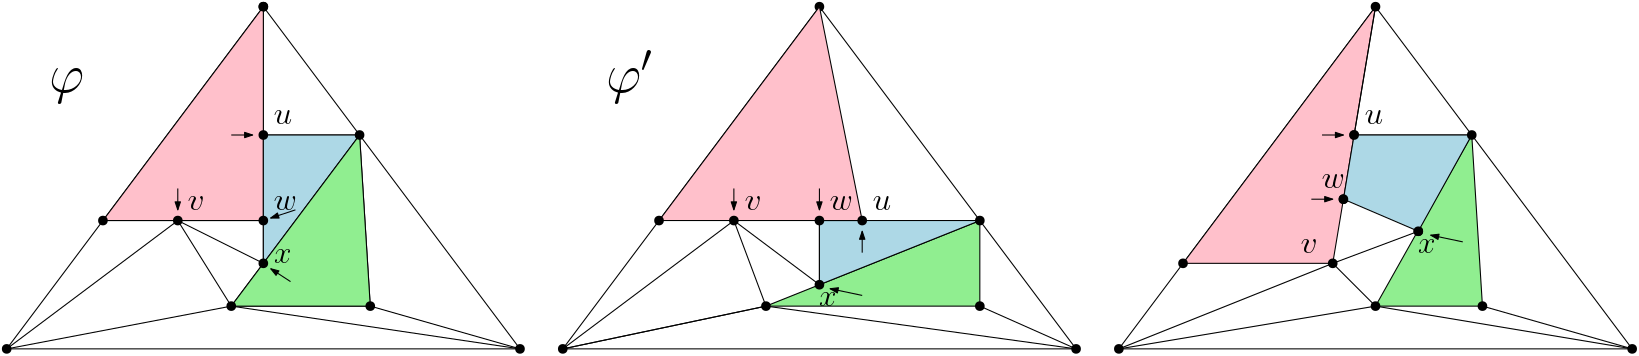
\includegraphics[width=0.9\textwidth]{lem_faa_choice_ex.png}
  	\caption{Die ganzzahligen Flüsse $\varphi$ und $\varphi'$ zusammen bilden den zulässigen Fluss $\frac{\varphi+\varphi'}{2}$, aber wir können nicht anfangen beliebige Winkel aus $\frac{\varphi_z+\varphi'_z}{2}$ zu wählen, um ein FAA zu erhalten. Rechts bleibt kein Knoten für das blaue Gebiet übrig.}
	\label{lem_faa_choice_ex}
\end{figure}

Wenn wir zeigen können, dass ein wie Lemma \ref{lem_faa} konstruiertes $\phi$ ein Gutes-FAA ist, folgt Vermutung \ref{int_conj}, da die Existenz eines Guten-FAAs $\phi$ nach Theorem \ref{theo_algo} auch die Existenz eines ganzzahligen zulässigen Flusses $\varphi$ für $\mathcal{N}_G$ impliziert.

\subsection{Minimale Schnitte in $\mathcal{N}_G$}

Angenommen, es existiert ein Graph $G$, für den nur eine nicht ganzzahlige Lösung existiert. Sei $\tilde{\varphi}$ dieser nicht ganzzahlige zulässige Fluss auf $\mathcal{N}_G$, und $\phi$ ein wie in Lemma \ref{lem_faa} aus $\tilde{\varphi}$ konstruiertes FAA für $G$. Sei $\overline{\varphi}_z$ der eindeutige Zuweisungs-Fluss der dieses FAA auf $\mathcal{N}_G$ kodiert. Sei $\overline{\mathcal{N}}_G$, ein Teilnetzwerk von $\mathcal{N}_G$, aus welchem alle Kanten, die von $\overline{\varphi}_z$ genutzt werden gelöscht wurden. Die Bedarfe sind weiterhin $|E_{in}|$ und $3|F_{in}|$ für den Schnyder- und Ecken-Fluss. Nach der in O1 festgehaltenen Beobachtung können wir, wie in \cite{af15}, $\varphi_s$ und $\varphi_e$ zusammenfassen und mit $\varphi_1$ bezeichnen. Wir suchen also nach einem zulässigem ganzzahligem Fluss $\varphi_1 = \varphi_s + \varphi_e$ auf $\overline{\mathcal{N}}_G$ mit Bedarf $|E_{in}| + 3|F_{in}|$, da dann auch eine ganzzahlige Lösung $(\varphi_s,\varphi_e)$ folgt.

Nach dem Max-Flow Min-Cut Theorem existiert ein zulässiger Fluss auf $\overline{\mathcal{N}}_G$ genau dann, wenn es keinen (Kanten-)Schnitt in $\overline{\mathcal{N}}_G$ mit Kapazität kleiner als $|E_{in}| + 3|F_{in}|$ gibt. Bevor wir fortfahren wollen wir einige Kantentypen aus $\mathcal{N}_G$ benennen.

\begin{itemize}
\item $E_\triangle = $ Die äusseren Kanten in den Winkeldreiecken.
\item $E_\triangledown = $ Die inneren Kanten in den Winkeldreiecken.
\item $S_* =$ Die Kanten von den Dummy-Knoten zur Dummy-Senke.
\item $V_* = $ Die Kanten von den Winkeldreiecken zu den Dummy-Knoten.
\item $E_{\to} = $ Die Kanten von Quelle 1 zu den Kanten-Knoten.
\item $F_\square = $ Die Kanten von den kleinen Quadraten zu inneren Gebieten $f$.
\item $V_{\to} = $ Die Kanten von den Knoten-Knoten zu Senke 1.
\end{itemize}

Sei $e_{d}$ die Kante von der Dummy-Senke zu Senke 2, dann sind sowohl $\mathcal{S}_1 = E_\triangle \cup E_{\to}$, als auch $\mathcal{S}_2 = F_\square \cup V_{\to} \cup \{e_{d}\}$ minimale Schnitte in $\mathcal{N}_G$, die alle Quellen und Senken trennen. Wenn wir nur von den Kanten aus $E_\triangle$, die in $\overline{\mathcal{N}}_G$ übrig sind, sprechen, schreiben wir $\overline{E}_\triangle$. Für die, zu diesen korrespondierenden Kanten im inneren ihrer Winkeldreiecke, schreiben wir $\overline{E}_\triangledown$. Für die Teilmengen von $V_*$ und $S_*$ in $\overline{\mathcal{N}}_G$ schreiben wir $\overline{S}_*$ und $\overline{V}_*$. Die restlichen Mengen sind vollständig in $\overline{\mathcal{N}}_G$ enthalten.

Seien $E_z$ die von $\overline{\varphi}_z$ genutzen Kanten, die wir aus $\mathcal{N}_G$ entfernen. Dann folgt $|\mathcal{S}_1 \cap E_z| = |E_\triangle \cap E_z| = |\varphi_z|$. Somit ist $\overline{\mathcal{S}}_1 = \mathcal{S}_1 \backslash E_z = \overline{E}_\triangle \cup E_\to$ ein Schnitt in $\overline{\mathcal{N}}_G$. Analog ist $\overline{\mathcal{S}}_2 = F_\square \cup V_{\to}$ ein Schnitt. Für die Kapazität von $\overline{\mathcal{S}}_1$ können wir folgern 
$$ c(\overline{\mathcal{S}}_1) = c(\overline{E}_\triangle) + c(E_\to) = c(E_\triangle) - |\varphi_z| + c(E_\to) = 3|F_{in}| + |E_{in}|,$$
und analog folgt $c(\overline{\mathcal{S}}_2) = 3|F_{in}| + |E_{in}|$.

Falls es sich hierbei um minimale Schnitte handelt, dann würde dies bedeuten, dass eine ganzzahlige Lösung für $\overline{\mathcal{N}}_G$ existiert, mit deren Hilfe wir, zusammen mit $\varphi_z$, eine ganzzahlige zulässige Lösung für $\mathcal{N}_G$ konstruieren könnten, was wiederum ein Widerspruch zu unserer Annahme wäre. Es muss also einen kleineren Schnitt $\mathcal{S}_{min}$, mit $|\mathcal{S}_{min}| \leq 3|F_{in}| + |E_{in}| - 1$, geben. 

\begin{claim} \label{cut_types1}

Ein minimaler Schnitt $\mathcal{S}_{min}$ in $\overline{\mathcal{N}}_G$ enthält ohne Beschränkung der Allgemeinheit nur Kanten von einem der vier Typen $\overline{E}_\triangledown, F_\square, V_\to$ und $E_\to$.

\end{claim}

Kanten auf einem Pfad von der Quelle bis zu einer Kante in $\overline{E}_\triangledown$, können durch diese ersetzt werden. Ebenso können Kanten zwischen zwei Winkeldreiecken, oder von einem Winkeldreieck zu einem kleinen Quadrat, durch die, entgegen dem Uhrzeigersinn, nächste Kante in $\overline{E}_\triangledown$ ersetzt werden. Kanten zwischen einem Kanten-Knoten und einem Knoten-Knoten, oder einem kleinen Quadrat, können durch eine Kante in $E_\to$ ersetzt werden. Abschliessend können Kanten, von einem inneren Gebiet zu Senke, durch das hinzufügen von allen Kanten aus $F_\square$ an diesem Gebiet, ersetzt werden.

\begin{figure}[h]
	\centering
  	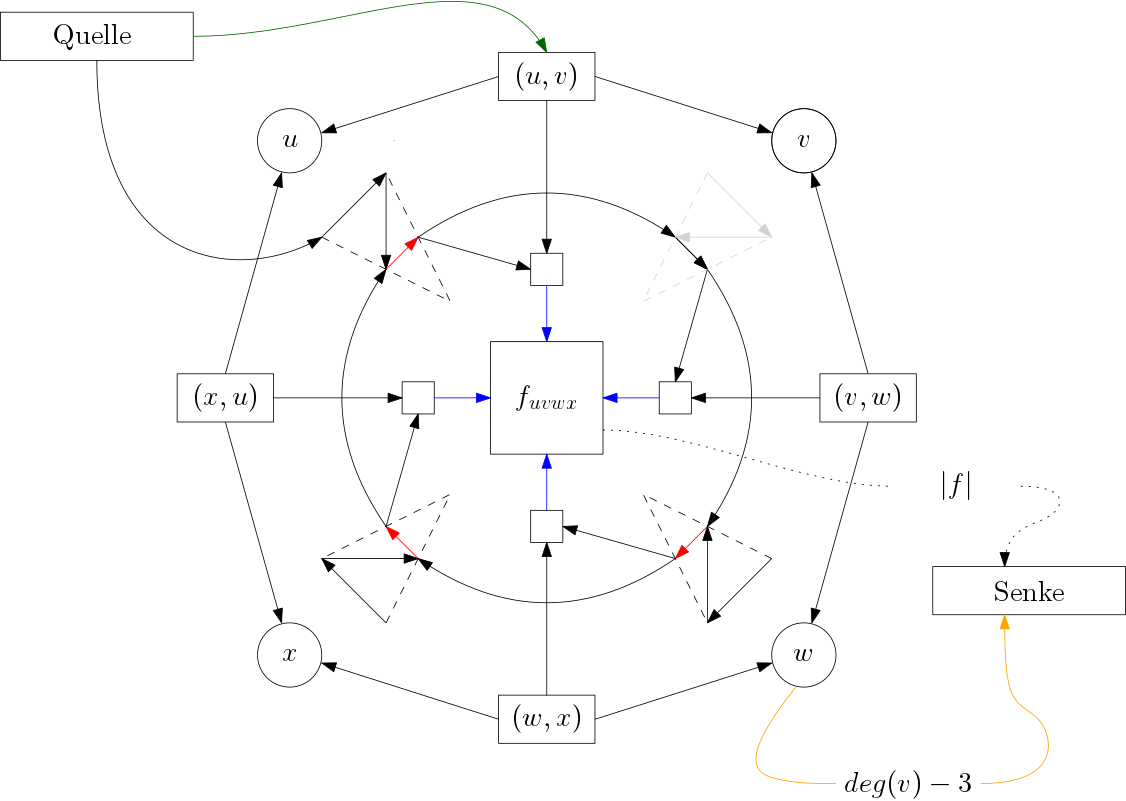
\includegraphics[width=0.7\textwidth]{face_cut.png}
  	\caption{Die vier Kantentypen $\overline{E}_\triangledown$ (rot), $F_\square$ (blau), $V_\to$ (orange) und $E_\to$ (grün) aus denen sich, nach Behauptungen \ref{cut_types1} und \ref{cut_types2}, ein minimaler Schnitt in $\overline{\mathcal{N}}_G$ zusammensetzt.}
\end{figure}

\begin{claim}\label{cut_types2}

Ein minimaler Schnitt $\mathcal{S}_{min}$ in $\overline{\mathcal{N}}_G$ muss ohne Beschränkung der Allgemeinheit aus jeder der Mengen $\overline{E}_\triangledown, F_\square, V_\to$ und $E_\to$ mindestens eine, aber aus keiner der Mengen alle Kanten enthalten.

\end{claim}

Falls ein solcher ein Schnitt existiert, dann kann er nicht alle Kanten $\overline{E}_\triangledown$ enthalten, da sonst $\mathcal{S}_{min} \cup (E_\triangle \cap E_z) \supseteq \mathcal{S}_1$ gilt. Falls er jedoch keine Kante aus $\overline{E}_\triangledown$ enthält, dann muss er alle Kanten aus $F_\square$ enthalten und falls er alle Kanten aus $F_\square$ enthält, dann muss er o.B.d.A. auch alle Kanten aus $V_\to$ enthalten. Es folgt $\mathcal{S}_{min} \cup \{e_d\} \supseteq \mathcal{S}_2$. Angenommen er enthält keine Kante aus $F_\square$, dann muss er alle Kanten aus $\overline{E}_\triangledown$ und $E_\to$ enthalten und es gilt $\mathcal{S}_{min} \cup (E_\triangle \cap E_z) \supseteq \mathcal{S}_1$. Mit analogen Argumenten folgt der Rest von Behauptung \ref{cut_types2}. \\

Nehmen wir also an, dass ein minimaler Schnitt $\mathcal{S}_{min}$, wie in Behauptungen \ref{cut_types1} und \ref{cut_types2}, existiert mit $|\mathcal{S}_{min}| \leq 3|F_{in}| + |E_{in}| - 1$. Betrachten wir für den Moment das Teilnetzwerk um ein inneres Gebiet in $\overline{\mathcal{N}}_G$. Falls alle drei Kanten aus $\overline{E}_\triangledown$ in $\mathcal{S}_{min}$ enthalten sind, dann müssen auch o.B.d.A alle Kanten in $E_\to$ um dieses Gebiet enthalten sein und falls eine Kante aus $\overline{E}_\triangledown$ nicht enthalten ist, dann müssen, im Uhrzeigersinn bis zur nächsten enthaltenen Kante aus $\overline{E}_\triangledown$, alle Kanten aus $F_\square$ Teil von $\mathcal{S}_{min}$ sein. Falls höchstens eine Kante aus $\overline{E}_\triangledown$ im Schnitt läge, dann folgt o.B.d.A, dass keine Kante aus $\overline{E}_\triangledown$ und alle aus $F_\square$, um das innere Gebiet, enthalten sind. 

Angenommen es existieren nur Gebiete in denen entweder alle oder keine Kanten aus $\overline{E}_\triangledown$ in $\mathcal{S}_{min}$ enthalten sind. Dann existiert ein Kanten-Knoten der, wie in Abbildung \ref{face_cut_edge} jeweils eines von beiden berührt. Wir können nun im rechten Gebiet eine Kante aus $F_\square$ durch die, entgegen dem Uhrzeigersinn, folgende Kante aus $\overline{E}_\triangledown$ ersetzen.

Sei $f$ ein Gebiet, 

\begin{figure}[h]
	\centering
  	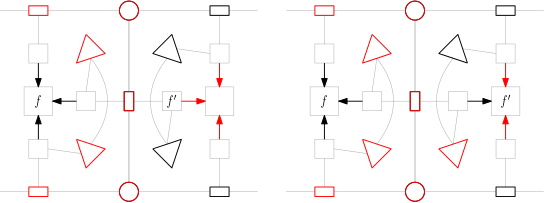
\includegraphics[width=1\textwidth]{sketch_cut.png}
  	\caption{}
	\label{face_cut_edge}
\end{figure}

\begin{lemma}\label{lem_min_cut}
Sei $\mathcal{N}$ ein gerichtetes Netzwerk mit einer Quelle $s$ und einer Senke $t$. Sei $\mathcal{S}_{min}$ ein minimaler Kantenschnitt zwischen $s$ und $t$ und sei $\mathcal{T} \subseteq \mathcal{S}_{min}$. Dann ist $\tilde{\mathcal{S}}_{min} = \mathcal{S}_{min} \backslash \mathcal{T}$ ein minimaler Kantenschnitt zwischen $s$ und $t$ in $\tilde{\mathcal{N}} = \mathcal{N}\backslash \mathcal{T}$.
\end{lemma}

\begin{proof}
Nehmen wir ohne Beschränkung der Allgemeinheit an, dass $\mathcal{N}$ nur Kanten mit Kapazität 1 enthält. Nach dem \textit{Max-Flow Min-Cut} Theorem existiert ein $s$-$t$-Fluss $\varphi$ mit $|\varphi| = c(\mathcal{S}_{min})$. Nach Theorem \ref{theo_int_flow} können wir annehmen, dass wir es sich um einen ganzzahligen Fluss handelt. Wir können diesen Fluss somit in Pfade (TODO) $p$ mit Flussstärke 1 aufteilen. Betrachten wir nun $\tilde{\mathcal{N}} = \mathcal{N} \backslash \mathcal{T}$, dann trennt die Entnahme von $\mathcal{T}$ genau $c(\mathcal{T})$ Pfade $p \in P$. Die restlichen Pfade, nennen wir sie $\tilde{p} \in \tilde{P}$, bleiben intakt. Somit existiert ein $s$-$t$-Fluss $\tilde{\varphi}$ mit $|\tilde{\varphi}| = c(\mathcal{S}_{min}) - c(\mathcal{T})$. $\tilde{\mathcal{S}}_{min} = \mathcal{S}_{min} \backslash \mathcal{T}$ muss somit ein minimaler Schnitt in $\tilde{\mathcal{N}}$ sein, da jedes $p \in \tilde{P}$ genau eine Kante aus $\tilde{\mathcal{S}}_{min}$ nutzt und die Entnahme dieser Kanten, nach Voraussetzung, $s$ und $t$ trennt.
\end{proof}


\begin{figure}
\centering
\begin{subfigure}{.4\textwidth}
  \centering
  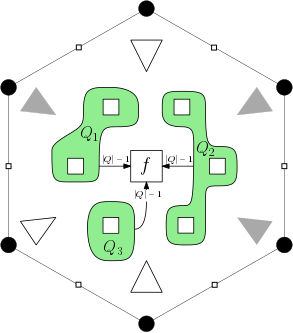
\includegraphics[width=0.9\linewidth]{6_face.png}
\end{subfigure}%
\begin{subfigure}{.6\textwidth}
  \centering
  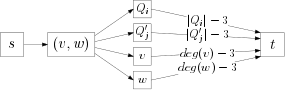
\includegraphics[width=0.9\linewidth]{schnyder_flow_non_int.png}
\end{subfigure}
\caption{Auf der linken Seite eine Illustration von $\overline{\varphi}_s$ mit den von $\overline{\varphi}_z$ zugeordneten Winkeln in grau. Auf der rechten Seite das resultierende Netzwerk.}
\end{figure}



\section{Nicht ganzzahlige Lösungen}

Dieses Kapitel wird sich mit der von Aerts und Felsner offen gelassenen Frage beschäftigen, ob die Erkennung von Graphen mit einer SLTR in $\mathcal{P}$ liegt. Wie in Kapitel \ref{pre} erwähnt, impliziert eine nicht ganzzahlige Lösung für ein Multi-Fluss-Problem auf einem gerichteten Graphen mit $n\geq 2$ Paaren von Quellen und Senken, im Allgemeinen nicht die Existenz einer ganzzahligen Lösung. Die Ergebnisse aus Kapitel \ref{the_program} lassen jedoch die Möglichkeit offen, dass das man für das betrachtete Netzwerk $\mathcal{N}_G$ die folgende Vermutung beweisen kann.

\begin{conjecture}\label{int_conj}
Sei $\tilde{\varphi}=(\tilde{\varphi_1},\tilde{\varphi_2})$ ein nicht ganzzahliger zulässiger Fluss auf $\mathcal{N}_G$, dann existiert auch ein ganzzahliger zulässiger Fluss $\varphi$ und wir können in polynomieller Zeit ein Gutes-FAA aus $\tilde{\varphi_2}$ extrahieren, ohne eine ganzzahlige Lösung zu berechnen.
\end{conjecture}

\begin{remark}
Wenn wir nicht darauf bestehen, dass unsere Lösung ganzzahlig ist, dann lässt sich eine Lösung nach TODO durch lineare Programmierung in polynomineller Zeit finden und das Entscheidungsproblem, ob ein Graph eine SLTR hat läge so in $\mathcal{P}$.
\end{remark}

Um die Argumentation einfacher zu gestalten, werden wir unser 2-Fluss Problem manchmal als 3-Fluss Problem, mit einer Lösung $\varphi=(\varphi_s,\varphi_e,\varphi_z)$, betrachten. Wir erstellen $\mathcal{N}^*_G$ wie zuvor $\mathcal{N}_G$, nur mit drei Quellen und Senken und weisen {Schnyder-,} Ecken-, und Zuweisungs-Fluss eigene Typen zu. Man kann leicht sehen, dass Theorem \ref{theo_algo} in angepasster Form hier ebenfalls gilt und ein zulässiger  Fluss $(\varphi_s,\varphi_z,\varphi_e)$ auf $\mathcal{N}_G^*$ genau dann existiert, wenn auch ein zulässiger Fluss $(\varphi_1,\varphi_2)$ auf $\mathcal{N}_G$ möglich ist. Die Hinrichtung ist klar. Nehmen wir an $(\varphi_1,\varphi_2)$ ist eine ganzzahlige Lösung. Nach Beobachtung A2 gilt, dass die äusseren Kanten eines Winkel-Dreiecks entweder von einem Ecken- oder einem Zuweisungs-Pfad genutzt werden. Diese Kanten sind zusammen mit den Kanten von Quelle 2 zu den Winkeldreiecken die einzigen in $\mathcal{N}_G$, die von beiden Flüssen genutzt werden. Wir können also $\varphi_2$ in $|\varphi_2|$ ganzzahlige Pfade aufteilen und jeden Pfad entweder $\varphi_e$ oder $\varphi_z$ zuweisen -- je nachdem ob er über die Dummy-Senke führt, oder nicht. Insbesondere folgt mit der gleichen Argumentation:

\begin{itemize}
\item [O1] Jede beliebige Kombination von $\varphi_s,\varphi_e$ und $\varphi_z$ zu zwei Flüssen und ein zu $\mathcal{N}_G$ analoges Netzwerk hat eine zulässige ganzzahlige Lösung genau dann, wenn eine Lösung für das 3-Fluss-Netzwerk existiert.
\end{itemize}

Betrachten wir zunächst den zweiten Teil von Vermutung \ref{int_conj}.

\begin{lemma}\label{lem_faa}
Sei $\tilde{\varphi}$ ein nicht ganzzahliger zulässiger Fluss auf $\mathcal{N}_G$ und sei $W$ die Menge der vom Zuweisungsfluss $\tilde{\varphi}_z$ genutzten inneren Winkel von $G$. Dann existiert eine Teilmenge $\phi\subseteq W$, sodass aus jedem Gebiet $f$ genau $|f|-3$ Winkel in $\phi$ enthalten sind und in der jeder Knoten $v$ höchstens einmal vorkommt. $\phi$ kodiert also ein FAA von $G$.
\end{lemma}

\begin{proof}
Wir betrachten das gerichtete Netzwerk $\mathcal{F}_z$ mit einer Quelle $s$ und Senke $t$, einem Beutel $B_f$ für jedes innere Gebiet $f$, einem Knoten $(f,v)$ für jeden inneren Winkel und einem Knoten für jeden Dummy-Knoten. Zuerst fügen Kanten mit Kapazität $|f|-3$ von der Quelle zu jedem Beutel ein. Dann folgen Kanten von den Beuteln $B_f$ zu den Winkeln von $f$, von den Winkeln $(f,v)$ zu den Dummy-Knoten $v^*$ und zuletzt eine Kante von jedem Dummy-Knoten zu Senke mit Kapazität 1, jeweils mit Kapazität 1. Der maximal mögliche $s$-$t$-Fluss in $\mathcal{F}_z$ ist $\sum_{f \in F_{in}}(|f|-3)$, da die Kanten zu den Beuteln einen Schnitt bilden und wir  aus $\tilde{\varphi}_z$ sofort eine zulässige nicht ganzzahlige Lösung $\tilde{\phi}$ für $\mathcal{F}_z$ konstruieren können. Nach Theorem \ref{theo_int_flow} existiert somit ein ganzzahliger Fluss $\phi$ auf $\mathcal{F}_z$, mit $|\phi| = |\tilde{\phi}| = |\tilde{\varphi}_z| = \sum_{f \in F_{in}}(|f|-3).$

\begin{figure}
	\centering
  	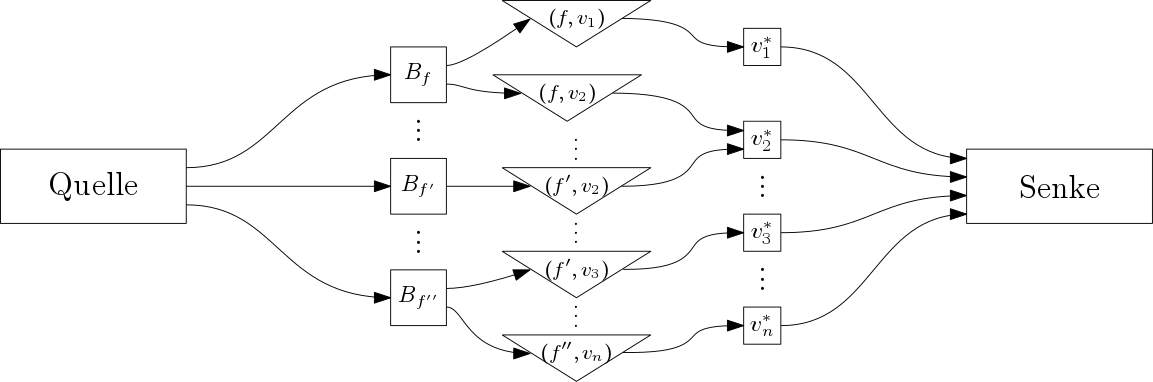
\includegraphics[width=0.7\textwidth]{lem_faa_choice.png}
  	\caption{Skizze des Netzwerkes $\mathcal{F}_z$. Die Kanten von der Quelle zu einem Beutel $B_f$ hat Kapazität $|f|-3$ und alle anderen haben Kapazität 1.}
\end{figure}

$\phi$ weißt nun jedem inneren Gebiet $f$ genau $|f|-3$ Winkel zu und jeder Knoten $v$ kann nur einmal zugewiesen werden. Wenn wir noch die per Konstruktion von $\mathcal{N}_G$ zugewiesenen Knoten am äusseren Gebiet hinzunehmen, dann kodiert $\phi$ ein FAA von $G$.
\end{proof}

\begin{remark}
Es ist uns nicht möglich mit beliebigen Winkeln aus $W$ zu beginnen und Schritt für Schritt für jedes Gebiet $|f|-3$ Winkel wählen, wie in Abbildung \ref{lem_faa_choice_ex} illustriert ist.
\end{remark}
\begin{figure}[h]
	\centering
  	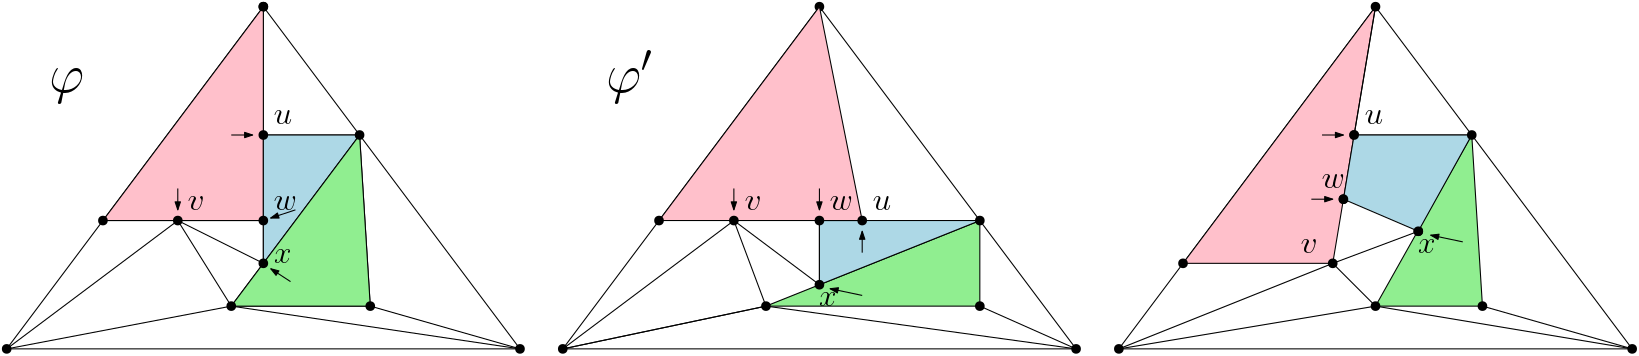
\includegraphics[width=0.9\textwidth]{lem_faa_choice_ex.png}
  	\caption{Die ganzzahligen Flüsse $\varphi$ und $\varphi'$ zusammen bilden den zulässigen Fluss $\frac{\varphi+\varphi'}{2}$, aber wir können nicht anfangen beliebige Winkel aus $\frac{\varphi_z+\varphi'_z}{2}$ zu wählen, um ein FAA zu erhalten. Rechts bleibt kein Knoten für das blaue Gebiet übrig.}
	\label{lem_faa_choice_ex}
\end{figure}

Wenn wir zeigen können, dass ein wie Lemma \ref{lem_faa} konstruiertes $\phi$ ein Gutes-FAA ist, folgt Vermutung \ref{int_conj}, da die Existenz eines Guten-FAAs $\phi$ nach Theorem \ref{theo_algo} auch die Existenz eines ganzzahligen zulässigen Flusses $\varphi$ für $\mathcal{N}_G$ impliziert.

\subsection{Minimale Schnitte in $\mathcal{N}_G$}

Angenommen, es existiert ein Graph $G$, für den nur eine nicht ganzzahlige Lösung existiert. Sei $\tilde{\varphi}$ dieser nicht ganzzahlige zulässige Fluss auf $\mathcal{N}_G$, und $\phi$ ein wie in Lemma \ref{lem_faa} aus $\tilde{\varphi}$ konstruiertes FAA für $G$. Sei $\overline{\varphi}_z$ der eindeutige Zuweisungs-Fluss der dieses FAA auf $\mathcal{N}_G$ kodiert. Sei $\overline{\mathcal{N}}_G$, ein Teilnetzwerk von $\mathcal{N}_G$, aus welchem alle Kanten, die von $\overline{\varphi}_z$ genutzt werden gelöscht wurden. Die Bedarfe sind weiterhin $|E_{in}|$ und $3|F_{in}|$ für den Schnyder- und Ecken-Fluss. Nach der in O1 festgehaltenen Beobachtung können wir, wie in \cite{af15}, $\varphi_s$ und $\varphi_e$ zusammenfassen und mit $\varphi_1$ bezeichnen. Wir suchen also nach einem zulässigem ganzzahligem Fluss $\varphi_1 = \varphi_s + \varphi_e$ auf $\overline{\mathcal{N}}_G$ mit Bedarf $|E_{in}| + 3|F_{in}|$, da dann auch eine ganzzahlige Lösung $(\varphi_s,\varphi_e)$ folgt.

Nach dem Max-Flow Min-Cut Theorem existiert ein zulässiger Fluss auf $\overline{\mathcal{N}}_G$ genau dann, wenn es keinen (Kanten-)Schnitt in $\overline{\mathcal{N}}_G$ mit Kapazität kleiner als $|E_{in}| + 3|F_{in}|$ gibt. Bevor wir fortfahren wollen wir einige Kantentypen aus $\mathcal{N}_G$ benennen.

\begin{itemize}
\item $E_\triangle = $ Die äusseren Kanten in den Winkeldreiecken.
\item $E_\triangledown = $ Die inneren Kanten in den Winkeldreiecken.
\item $S_* =$ Die Kanten von den Dummy-Knoten zur Dummy-Senke.
\item $V_* = $ Die Kanten von den Winkeldreiecken zu den Dummy-Knoten.
\item $E_{\to} = $ Die Kanten von Quelle 1 zu den Kanten-Knoten.
\item $F_\square = $ Die Kanten von den kleinen Quadraten zu inneren Gebieten $f$.
\item $V_{\to} = $ Die Kanten von den Knoten-Knoten zu Senke 1.
\end{itemize}

Sei $e_{d}$ die Kante von der Dummy-Senke zu Senke 2, dann sind sowohl $\mathcal{S}_1 = E_\triangle \cup E_{\to}$, als auch $\mathcal{S}_2 = F_\square \cup V_{\to} \cup \{e_{d}\}$ minimale Schnitte in $\mathcal{N}_G$, die alle Quellen und Senken trennen. Wenn wir nur von den Kanten aus $E_\triangle$, die in $\overline{\mathcal{N}}_G$ übrig sind, sprechen, schreiben wir $\overline{E}_\triangle$. Für die, zu diesen korrespondierenden Kanten im inneren ihrer Winkeldreiecke, schreiben wir $\overline{E}_\triangledown$. Für die Teilmengen von $V_*$ und $S_*$ in $\overline{\mathcal{N}}_G$ schreiben wir $\overline{S}_*$ und $\overline{V}_*$. Die restlichen Mengen sind vollständig in $\overline{\mathcal{N}}_G$ enthalten.

Seien $E_z$ die von $\overline{\varphi}_z$ genutzen Kanten, die wir aus $\mathcal{N}_G$ entfernen. Dann folgt $|\mathcal{S}_1 \cap E_z| = |E_\triangle \cap E_z| = |\varphi_z|$. Somit ist $\overline{\mathcal{S}}_1 = \mathcal{S}_1 \backslash E_z = \overline{E}_\triangle \cup E_\to$ ein Schnitt in $\overline{\mathcal{N}}_G$. Analog ist $\overline{\mathcal{S}}_2 = F_\square \cup V_{\to}$ ein Schnitt. Für die Kapazität von $\overline{\mathcal{S}}_1$ können wir folgern 
$$ c(\overline{\mathcal{S}}_1) = c(\overline{E}_\triangle) + c(E_\to) = c(E_\triangle) - |\varphi_z| + c(E_\to) = 3|F_{in}| + |E_{in}|,$$
und analog folgt $c(\overline{\mathcal{S}}_2) = 3|F_{in}| + |E_{in}|$.

Falls es sich hierbei um minimale Schnitte handelt, dann würde dies bedeuten, dass eine ganzzahlige Lösung für $\overline{\mathcal{N}}_G$ existiert, mit deren Hilfe wir, zusammen mit $\varphi_z$, eine ganzzahlige zulässige Lösung für $\mathcal{N}_G$ konstruieren könnten, was wiederum ein Widerspruch zu unserer Annahme wäre. Es muss also einen kleineren Schnitt $\mathcal{S}_{min}$, mit $|\mathcal{S}_{min}| \leq 3|F_{in}| + |E_{in}| - 1$, geben. 

\begin{claim} \label{cut_types1}

Ein minimaler Schnitt $\mathcal{S}_{min}$ in $\overline{\mathcal{N}}_G$ enthält ohne Beschränkung der Allgemeinheit nur Kanten von einem der vier Typen $\overline{E}_\triangledown, F_\square, V_\to$ und $E_\to$.

\end{claim}

Kanten auf einem Pfad von der Quelle bis zu einer Kante in $\overline{E}_\triangledown$, können durch diese ersetzt werden. Ebenso können Kanten zwischen zwei Winkeldreiecken, oder von einem Winkeldreieck zu einem kleinen Quadrat, durch die, entgegen dem Uhrzeigersinn, nächste Kante in $\overline{E}_\triangledown$ ersetzt werden. Kanten zwischen einem Kanten-Knoten und einem Knoten-Knoten, oder einem kleinen Quadrat, können durch eine Kante in $E_\to$ ersetzt werden. Abschliessend können Kanten, von einem inneren Gebiet zu Senke, durch das hinzufügen von allen Kanten aus $F_\square$ an diesem Gebiet, ersetzt werden.

\begin{figure}[h]
	\centering
  	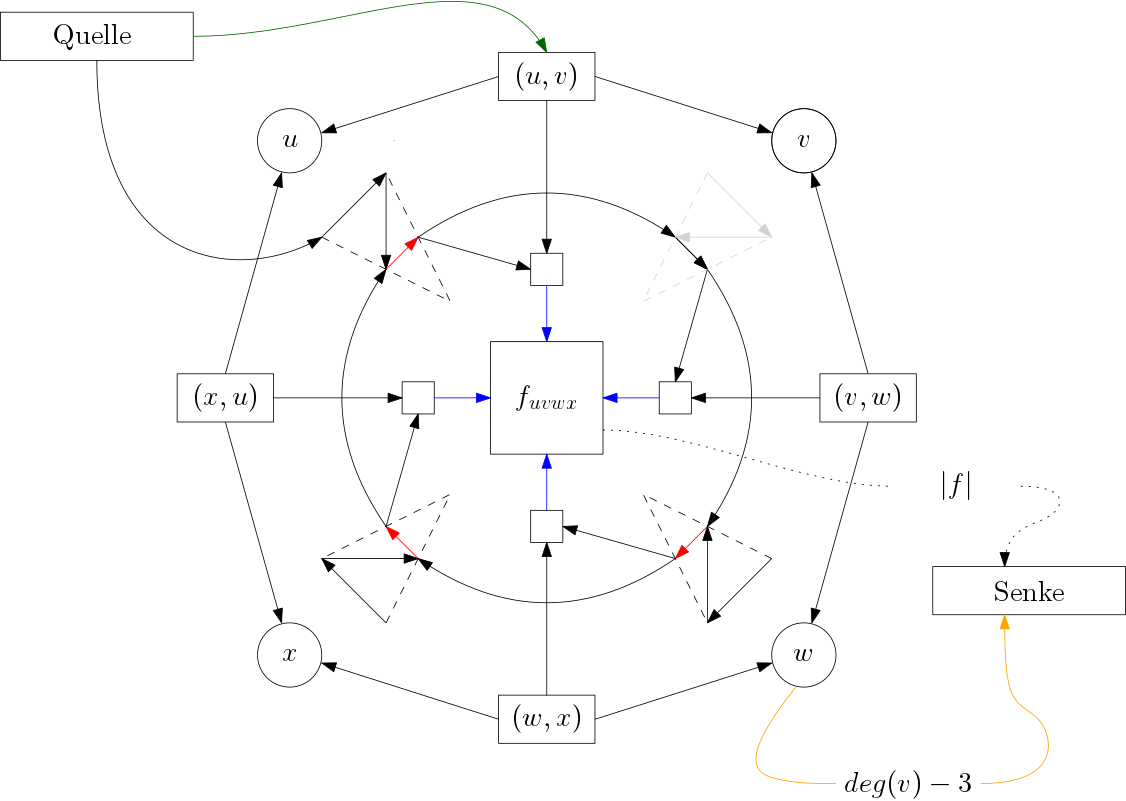
\includegraphics[width=0.7\textwidth]{face_cut.png}
  	\caption{Die vier Kantentypen $\overline{E}_\triangledown$ (rot), $F_\square$ (blau), $V_\to$ (orange) und $E_\to$ (grün) aus denen sich, nach Behauptungen \ref{cut_types1} und \ref{cut_types2}, ein minimaler Schnitt in $\overline{\mathcal{N}}_G$ zusammensetzt.}
\end{figure}

\begin{claim}\label{cut_types2}

Ein minimaler Schnitt $\mathcal{S}_{min}$ in $\overline{\mathcal{N}}_G$ muss ohne Beschränkung der Allgemeinheit aus jeder der Mengen $\overline{E}_\triangledown, F_\square, V_\to$ und $E_\to$ mindestens eine, aber aus keiner der Mengen alle Kanten enthalten.

\end{claim}

Falls ein solcher ein Schnitt existiert, dann kann er nicht alle Kanten $\overline{E}_\triangledown$ enthalten, da sonst $\mathcal{S}_{min} \cup (E_\triangle \cap E_z) \supseteq \mathcal{S}_1$ gilt. Falls er jedoch keine Kante aus $\overline{E}_\triangledown$ enthält, dann muss er alle Kanten aus $F_\square$ enthalten und falls er alle Kanten aus $F_\square$ enthält, dann muss er o.B.d.A. auch alle Kanten aus $V_\to$ enthalten. Es folgt $\mathcal{S}_{min} \cup \{e_d\} \supseteq \mathcal{S}_2$. Angenommen er enthält keine Kante aus $F_\square$, dann muss er alle Kanten aus $\overline{E}_\triangledown$ und $E_\to$ enthalten und es gilt $\mathcal{S}_{min} \cup (E_\triangle \cap E_z) \supseteq \mathcal{S}_1$. Mit analogen Argumenten folgt der Rest von Behauptung \ref{cut_types2}. \\

Nehmen wir also an, dass ein minimaler Schnitt $\mathcal{S}_{min}$, wie in Behauptungen \ref{cut_types1} und \ref{cut_types2}, existiert mit $|\mathcal{S}_{min}| \leq 3|F_{in}| + |E_{in}| - 1$. Betrachten wir für den Moment das Teilnetzwerk um ein inneres Gebiet in $\overline{\mathcal{N}}_G$. Falls alle drei Kanten aus $\overline{E}_\triangledown$ in $\mathcal{S}_{min}$ enthalten sind, dann müssen auch o.B.d.A alle Kanten in $E_\to$ um dieses Gebiet enthalten sein und falls eine Kante aus $\overline{E}_\triangledown$ nicht enthalten ist, dann müssen, im Uhrzeigersinn bis zur nächsten enthaltenen Kante aus $\overline{E}_\triangledown$, alle Kanten aus $F_\square$ Teil von $\mathcal{S}_{min}$ sein. Falls höchstens eine Kante aus $\overline{E}_\triangledown$ im Schnitt läge, dann folgt o.B.d.A, dass keine Kante aus $\overline{E}_\triangledown$ und alle aus $F_\square$, um das innere Gebiet, enthalten sind. 

Angenommen es existieren nur Gebiete in denen entweder alle oder keine Kanten aus $\overline{E}_\triangledown$ in $\mathcal{S}_{min}$ enthalten sind. Dann existiert ein Kanten-Knoten der, wie in Abbildung \ref{face_cut_edge} jeweils eines von beiden berührt. Wir können nun im rechten Gebiet eine Kante aus $F_\square$ durch die, entgegen dem Uhrzeigersinn, folgende Kante aus $\overline{E}_\triangledown$ ersetzen.

Sei $f$ ein Gebiet, 

\begin{figure}[h]
	\centering
  	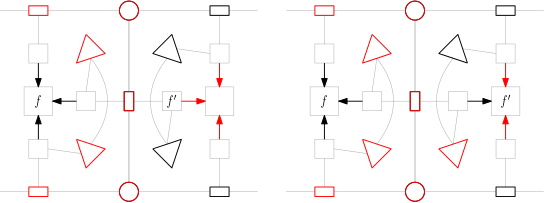
\includegraphics[width=1\textwidth]{sketch_cut.png}
  	\caption{}
	\label{face_cut_edge}
\end{figure}

\begin{lemma}\label{lem_min_cut}
Sei $\mathcal{N}$ ein gerichtetes Netzwerk mit einer Quelle $s$ und einer Senke $t$. Sei $\mathcal{S}_{min}$ ein minimaler Kantenschnitt zwischen $s$ und $t$ und sei $\mathcal{T} \subseteq \mathcal{S}_{min}$. Dann ist $\tilde{\mathcal{S}}_{min} = \mathcal{S}_{min} \backslash \mathcal{T}$ ein minimaler Kantenschnitt zwischen $s$ und $t$ in $\tilde{\mathcal{N}} = \mathcal{N}\backslash \mathcal{T}$.
\end{lemma}

\begin{proof}
Nehmen wir ohne Beschränkung der Allgemeinheit an, dass $\mathcal{N}$ nur Kanten mit Kapazität 1 enthält. Nach dem \textit{Max-Flow Min-Cut} Theorem existiert ein $s$-$t$-Fluss $\varphi$ mit $|\varphi| = c(\mathcal{S}_{min})$. Nach Theorem \ref{theo_int_flow} können wir annehmen, dass wir es sich um einen ganzzahligen Fluss handelt. Wir können diesen Fluss somit in Pfade (TODO) $p$ mit Flussstärke 1 aufteilen. Betrachten wir nun $\tilde{\mathcal{N}} = \mathcal{N} \backslash \mathcal{T}$, dann trennt die Entnahme von $\mathcal{T}$ genau $c(\mathcal{T})$ Pfade $p \in P$. Die restlichen Pfade, nennen wir sie $\tilde{p} \in \tilde{P}$, bleiben intakt. Somit existiert ein $s$-$t$-Fluss $\tilde{\varphi}$ mit $|\tilde{\varphi}| = c(\mathcal{S}_{min}) - c(\mathcal{T})$. $\tilde{\mathcal{S}}_{min} = \mathcal{S}_{min} \backslash \mathcal{T}$ muss somit ein minimaler Schnitt in $\tilde{\mathcal{N}}$ sein, da jedes $p \in \tilde{P}$ genau eine Kante aus $\tilde{\mathcal{S}}_{min}$ nutzt und die Entnahme dieser Kanten, nach Voraussetzung, $s$ und $t$ trennt.
\end{proof}


\begin{figure}
\centering
\begin{subfigure}{.4\textwidth}
  \centering
  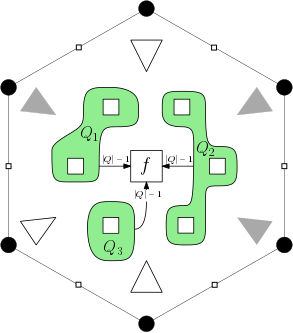
\includegraphics[width=0.9\linewidth]{6_face.png}
\end{subfigure}%
\begin{subfigure}{.6\textwidth}
  \centering
  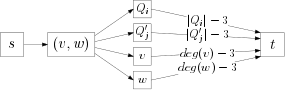
\includegraphics[width=0.9\linewidth]{schnyder_flow_non_int.png}
\end{subfigure}
\caption{Auf der linken Seite eine Illustration von $\overline{\varphi}_s$ mit den von $\overline{\varphi}_z$ zugeordneten Winkeln in grau. Auf der rechten Seite das resultierende Netzwerk.}
\end{figure}


\section{Das Programm}

Wir wollen in diesem Abschnitt eine Implementierung des Algorithmus analysieren und 

Wir wollen nun auf eine Implementierung des Algorithmus aus dem vorherigen Abschnitt eingehen. Der Code wurde in SageMath \cite{sage} geschrieben und ist auf Anfrage erhältlich. Ein Multi-Fluss wird hier mit Hilfe des in Sage enthaltenen Solvers Glpk \cite{glpk}, für Lineare Programmierung gelößt. Bevor wir uns mit der Analyse von Daten auseinandersetzten aber zuvor noch ein paar Worte zu möglichen und nicht möglichen Vereinfachungen.




\subsection{1-Fluss}

Wenn wir die Quellen und Senken vereinigen, würden wir ein 1-Fluss Netzwerk erhalten. Somit würde eine nicht ganzzahlige Lösung auch die  Existenz einer ganzzahlige Lösung und



safasdasd
\begin{figure}
        \centering
\begin{tikzpicture}[thick, scale=1.6,font=\tiny]
\begin{axis}[xlabel=Knoten,ylabel=Kanten]

\addplot[
	scatter/classes={
    	s={mark=square*,scale=0.2,black},
    	f={mark=square*,scale=0.2,green},
    	n={mark=square*,scale=0.2,blue}
    	},
	scatter,only marks,
    	scatter src=explicit symbolic,]
	table[meta=label] {
x y label
10 18 s
10 16 f
10 19 s
10 19 s
10 19 s
10 20 s
10 18 s
10 18 s
10 17 s
10 19 s
10 19 s
10 21 s
10 17 f
10 17 s
10 18 s
10 20 s
10 16 f
10 20 s
10 17 f
10 16 f
11 19 s
11 22 s
11 19 s
11 19 f
11 19 s
11 22 s
11 18 f
11 20 s
11 22 s
11 19 s
11 20 s
11 21 s
11 19 s
11 20 s
11 20 f
11 18 f
11 20 s
11 23 s
11 20 s
11 19 s
12 18 f
12 22 s
12 22 s
12 18 f
12 20 f
12 23 s
12 21 s
12 22 s
12 19 f
12 24 s
12 22 s
12 20 f
12 20 f
12 21 s
12 18 f
12 22 s
12 21 s
12 24 s
12 20 f
12 18 f
13 21 f
13 20 f
13 20 f
13 25 s
13 22 f
13 26 s
13 20 f
13 27 s
13 25 s
13 24 s
13 24 s
13 24 s
13 25 s
13 27 s
13 23 s
13 24 s
13 26 s
13 25 s
13 23 f
13 26 s
14 29 s
14 30 s
14 21 n
14 23 f
14 24 f
14 23 f
14 27 s
14 27 s
14 27 s
14 30 s
14 28 s
14 27 s
14 25 s
14 25 s
14 28 s
14 25 s
14 29 s
14 25 s
14 25 s
14 25 f
16 29 f
16 26 f
16 27 f
16 28 f
16 31 s
16 30 s
16 31 s
16 31 s
16 32 s
16 33 s
17 31 s
17 31 f
17 33 s
17 28 f
17 31 f
17 32 s
17 32 s
17 32 s
17 30 f
17 33 s
18 34 s
18 37 s
18 33 s
18 33 s
18 29 n
18 30 f
18 30 f
18 37 s
18 36 s
18 34 s
19 36 s
19 30 n
19 30 n
19 39 s
19 38 s
19 34 f
19 33 f
19 39 s
19 30 n
19 43 s
20 30 n
20 32 n
20 40 f
20 37 f
20 38 f
20 34 f
20 45 s
20 31 n
20 37 s
20 38 s
21 42 s
21 40 f
21 42 s
21 37 f
21 33 n
21 32 n
21 37 f
21 37 f
21 35 n
21 42 s
22 34 n
22 39 f
22 40 f
22 41 s
22 45 s
22 49 s
22 36 n
22 42 s
22 41 f
22 42 s
23 46 s
23 38 n
23 44 f
23 42 f
23 46 s
23 45 s
23 45 s
23 42 f
23 48 s
23 47 s
24 45 s
24 40 n
24 42 n
24 45 f
24 45 f
24 52 s
24 42 f
24 47 f
24 48 s
24 44 f
25 43 n
25 53 s
25 47 s
25 50 s
25 49 s
25 43 n
25 43 n
25 49 s
25 44 n
25 46 f
26 47 f
26 49 f
26 48 f
26 49 f
26 49 f
26 52 f
26 48 f
26 44 n
26 51 f
26 46 n
27 53 f
27 50 f
27 55 f
27 48 f
27 45 n
27 57 s
27 52 s
27 56 s
27 46 n
27 54 s
28 48 n
28 54 s
28 51 f
28 52 f
28 52 f
28 48 n
28 46 n
28 56 s
28 55 s
28 49 n
29 50 n
29 69 s
29 54 f
29 56 s
29 58 s
29 57 s
29 63 s
29 44 n
29 53 f
29 55 f
16 33 s
16 27 f
16 30 f
16 28 f
16 29 f
16 29 s
16 31 s
16 28 f
16 34 s
16 30 s
16 28 f
16 32 s
16 27 f
16 30 s
16 26 f
16 28 f
16 30 s
16 30 s
16 28 f
16 28 f
17 31 f
17 30 f
17 39 s
17 32 s
17 33 s
17 35 s
17 31 s
17 27 n
17 35 s
17 27 n
17 31 f
17 29 f
17 33 s
17 34 s
17 30 f
17 39 s
17 31 s
17 29 f
17 36 s
17 33 s
18 29 n
18 36 s
18 38 s
18 30 f
18 41 s
18 34 s
18 31 f
18 33 f
18 31 f
18 36 s
18 33 f
18 29 n
18 30 f
18 29 n
18 33 s
18 28 n
18 37 s
18 34 s
18 37 s
18 37 s
19 33 f
19 32 f
19 37 s
19 35 f
19 33 f
19 31 n
19 31 n
19 35 f
19 38 s
19 34 f
19 41 s
19 37 f
19 33 f
19 29 n
19 35 f
19 40 s
19 36 s
19 30 n
19 32 f
19 34 f
20 36 f
20 39 f
20 40 s
20 47 s
20 37 f
20 36 f
20 33 n
20 36 f
20 38 s
20 36 f
20 40 s
20 30 n
20 36 f
20 37 f
20 33 n
20 37 s
20 33 n
20 32 n
20 40 s
20 38 s
21 40 f
21 40 s
21 34 n
21 37 f
21 40 s
21 40 s
21 37 f
21 34 n
21 39 f
21 39 f
21 38 f
21 42 s
21 40 f
21 38 f
21 37 f
21 39 f
21 40 s
21 34 n
21 40 f
21 42 s
22 38 f
22 37 n
22 38 n
22 45 s
22 39 f
22 40 f
22 34 n
22 42 f
22 37 n
22 41 f
22 41 f
22 35 n
22 38 f
22 43 s
22 40 f
22 34 n
22 40 f
22 36 n
22 43 s
22 36 n
23 36 n
23 47 s
23 42 f
23 36 n
23 36 n
23 46 s
23 42 f
23 43 s
23 42 f
23 38 n
23 53 s
23 45 f
23 48 s
23 48 s
23 45 f
23 43 f
23 44 s
23 47 s
23 40 f
23 40 f
24 42 n
24 47 s
24 44 f
24 43 f
24 47 s
24 41 n
24 43 f
24 51 s
24 39 n
24 46 f
24 40 n
24 47 s
24 51 s
24 41 n
24 46 f
24 45 f
24 41 n
24 44 f
24 46 s
24 46 s
25 42 n
25 43 n
25 51 s
25 52 s
25 50 s
25 47 f
25 47 f
25 44 f
25 49 s
25 48 f
25 45 f
25 44 f
25 39 n
25 45 f
25 50 s
25 48 s
25 45 f
25 50 s
25 51 s
25 43 n
26 42 n
26 47 n
26 55 s
26 47 f
26 46 f
26 43 n
26 50 s
26 42 n
26 50 f
26 48 f
26 44 n
26 40 n
26 54 s
26 45 n
26 49 s
26 45 n
26 46 f
26 47 f
26 47 f
26 46 f
27 52 s
27 48 f
27 54 s
27 58 s
27 44 n
27 51 f
27 51 f
27 52 s
27 47 n
27 52 f
27 45 n
27 48 f
27 45 n
27 51 f
27 46 n
27 52 f
27 44 n
27 51 f
27 51 f
27 48 f
28 47 n
28 50 f
28 57 s
28 48 n
28 48 n
28 56 s
28 47 n
28 51 n
28 46 n
28 55 s
28 46 n
28 55 s
28 48 n
28 48 n
28 54 s
28 51 n
28 52 f
28 53 f
28 50 f
28 56 s
29 56 s
29 56 s
29 52 n
29 53 n
29 59 s
29 51 n
29 46 n
29 55 f
29 51 n
29 63 s
29 63 s
29 60 s
29 48 n
29 48 n
29 46 n
29 47 n
29 51 n
29 58 f
29 60 s
29 49 n
30 67 s
30 65 s
30 53 n
30 59 s
30 47 n
30 53 n
30 56 f
30 51 n
30 49 n
30 59 s
30 54 f
30 55 f
30 59 s
30 59 f
30 49 n
30 57 f
30 53 n
30 60 f
30 56 f
30 56 f
31 61 s
31 62 f
31 62 s
31 60 s
31 52 n
31 67 s
31 55 n
31 59 f
31 57 f
31 56 f
31 56 n
31 57 f
31 58 f
31 71 s
31 52 n
31 61 s
31 55 n
31 61 f
31 58 f
31 55 n
32 67 f
32 59 n
32 61 f
32 54 n
32 55 n
32 62 s
32 59 f
32 57 n
32 62 s
32 60 f
32 56 n
32 65 s
32 57 n
32 63 f
32 52 n
32 64 s
32 56 n
32 59 f
32 60 n
32 64 s
33 58 n
33 62 f
33 59 n
33 58 n
33 59 n
33 68 s
33 66 s
33 62 f
33 60 f
33 67 s
33 52 n
33 62 f
33 57 n
33 62 n
33 58 n
33 58 n
33 65 f
33 66 s
33 60 f
33 68 s
34 63 f
34 67 s
34 71 f
34 58 n
34 70 f
34 60 n
34 61 n
34 55 n
34 70 s
34 63 f
34 67 f
34 63 f
34 68 s
34 59 n
34 66 f
34 56 n
34 67 s
34 59 n
34 71 s
34 69 s
35 73 s
35 66 n
35 59 n
35 67 f
35 66 f
35 69 f
35 68 s
35 61 n
35 61 n
35 76 s
35 69 s
35 67 f
35 59 n
35 63 n
35 68 s
35 59 n
35 67 s
35 69 s
35 59 n
35 63 n
36 62 n
36 65 n
36 62 n
36 65 n
36 62 n
36 60 n
36 61 n
36 70 f
36 64 n
36 73 s
36 71 f
36 65 n
36 65 n
36 62 n
36 65 n
36 68 f
36 75 s
36 63 n
36 67 n
36 73 s
37 68 f
37 67 n
37 68 n
37 68 f
37 74 s
37 77 s
37 77 f
37 72 f
37 70 f
37 63 n
37 77 s
37 60 n
37 75 f
37 65 n
37 73 f
37 67 n
37 68 f
37 62 n
37 67 n
37 76 f
38 68 n
38 71 f
38 69 n
38 66 n
38 72 f
38 71 f
38 74 f
38 77 s
38 64 n
38 70 f
38 66 n
38 73 f
38 70 n
38 73 f
38 71 f
38 70 n
38 72 f
38 75 s
38 84 s
38 75 f
39 71 n
39 71 n
39 73 f
39 67 n
39 75 f
39 69 n
39 74 f
39 78 s
39 73 f
39 79 f
39 80 f
39 72 n
39 66 n
39 71 n
39 75 f
39 76 f
39 83 s
39 73 n
39 75 f
39 78 f
40 71 n
40 81 s
40 78 f
40 74 n
40 66 n
40 74 n
40 75 n
40 76 f
40 94 s
40 67 n
40 67 n
40 83 s
40 79 s
40 79 s
40 79 s
40 72 n
40 83 s
40 72 n
40 76 f
40 74 n
41 74 n
41 78 f
41 70 n
41 80 f
41 77 f
41 74 n
41 82 s
41 86 s
41 66 n
41 73 n
41 82 s
41 82 f
41 69 n
41 77 n
41 75 n
41 76 n
41 80 n
41 74 n
41 76 f
41 77 n
42 73 n
42 78 n
42 83 s
42 74 n
42 80 n
42 78 n
42 81 f
42 81 f
42 83 s
42 80 f
42 80 f
42 81 f
42 82 f
42 79 n
42 78 n
42 74 n
42 79 f
42 83 f
42 75 n
42 79 f
43 75 n
43 83 f
43 80 n
43 76 n
43 79 n
43 75 n
43 76 n
43 74 n
43 82 f
43 93 s
43 73 n
43 76 n
43 88 s
43 78 n
43 88 f
43 87 f
43 73 n
43 76 n
43 74 n
43 80 n
44 83 n
44 84 f
44 82 n
44 79 n
44 87 f
44 88 f
44 76 n
44 76 n
44 82 n
44 90 s
44 76 n
44 78 n
44 88 s
44 87 f
44 87 f
44 79 n
44 78 n
44 91 s
44 79 n
44 88 s
45 86 f
45 93 s
45 92 f
45 80 n
45 86 f
45 81 n
45 77 n
45 88 n
45 78 n
45 87 f
45 82 n
45 83 n
45 83 n
45 98 s
45 79 n
45 88 f
45 88 n
45 76 n
45 85 f
45 93 s
46 91 f
46 91 f
46 96 s
46 97 s
46 89 f
46 84 n
46 84 n
46 90 f
46 80 n
46 90 f
46 89 f
46 90 f
46 87 f
46 90 f
46 86 n
46 84 n
46 96 s
46 89 f
46 89 f
46 83 n
47 88 n
47 100 s
47 78 n
47 89 f
47 88 n
47 91 f
47 81 n
47 84 n
47 90 n
47 82 n
47 90 f
47 87 n
47 85 n
47 89 n
47 100 s
47 96 s
47 92 f
47 83 n
47 90 f
47 79 n
48 77 n
48 81 n
48 89 n
48 85 n
48 90 n
48 114 s
48 87 n
48 98 s
48 102 s
48 107 s
48 86 n
48 95 n
48 92 n
48 108 s
48 87 n
48 99 s
48 84 n
48 96 f
48 84 n
48 105 s
49 87 n
49 93 f
49 86 n
49 89 n
49 99 f
49 91 n
49 81 n
49 94 f
49 101 s
49 104 s
49 88 n
49 102 f
49 93 n
49 95 f
49 89 n
49 94 n
49 83 n
49 98 s
49 98 f
49 102 f
50 98 s
50 101 f
50 99 f
50 95 n
50 94 n
50 95 n
50 95 n
50 98 f
50 99 s
50 105 s
50 80 n
50 101 s
50 82 n
50 93 n
50 84 n
50 98 n
50 85 n
50 99 s
50 97 f
50 92 n
51 90 n
51 103 s
51 93 n
51 91 n
51 96 n
51 86 n
51 91 n
51 91 n
51 90 n
51 91 n
51 98 n
51 84 n
51 91 n
51 93 n
51 93 n
51 99 f
51 98 n
51 88 n
51 102 f
51 102 f
52 103 f
52 99 n
52 89 n
52 94 n
52 99 f
52 128 s
52 103 s
52 97 n
52 96 n
52 109 s
52 95 n
52 102 n
52 98 n
52 88 n
52 97 n
52 92 n
52 101 f
52 101 n
52 99 n
52 97 n
53 92 n
53 106 f
53 105 f
53 114 s
53 109 f
53 102 f
53 98 n
53 100 n
53 107 f
53 90 n
53 100 n
53 93 n
53 106 f
53 98 n
53 102 f
53 95 n
53 99 n
53 106 f
53 98 n
53 95 n
54 119 s
54 106 f
54 119 s
54 105 f
54 88 n
54 110 s
54 104 f
54 101 n
54 105 n
54 103 n
54 101 n
54 102 n
54 111 s
54 99 n
54 97 n
54 95 n
54 101 n
54 106 f
54 109 f
54 94 n
55 104 n
55 110 f
55 111 s
55 109 s
55 107 n
55 102 n
55 98 n
55 109 f
55 89 n
55 96 n
55 104 n
55 104 n
55 104 n
55 124 s
55 124 s
55 102 n
55 108 f
55 101 n
55 95 n
55 108 s
56 113 s
56 101 n
56 116 s
56 99 n
56 103 n
56 102 n
56 93 n
56 104 n
56 99 n
56 96 n
56 108 n
56 104 n
56 107 n
56 105 n
56 104 n
56 106 f
56 97 n
56 107 n
56 113 f
56 106 n
57 121 s
57 104 n
57 99 n
57 115 s
57 102 n
57 112 f
57 108 n
57 108 n
57 114 f
57 106 n
57 108 n
57 95 n
57 109 n
57 106 n
57 113 f
57 104 n
57 101 n
57 114 f
57 111 n
57 102 n
58 105 n
58 120 f
58 108 n
58 113 n
58 115 f
58 109 n
58 111 n
58 109 n
58 114 f
58 113 f
58 105 n
58 105 n
58 110 n
58 109 n
58 118 s
58 102 n
58 113 f
58 121 s
58 115 f
58 114 n
59 105 n
59 107 n
59 113 n
59 114 f
59 108 n
59 116 f
59 105 n
59 111 n
59 109 n
59 118 f
59 115 n
59 117 f
59 115 f
59 116 f
59 123 s
59 123 s
59 107 n
59 117 f
59 101 n
59 107 n
60 118 f
60 107 n
60 104 n
60 124 s
60 109 n
60 102 n
60 114 n
60 119 n
60 112 n
60 111 n
60 108 n
60 119 f
60 113 n
60 118 n
60 114 n
60 116 n
60 115 f
60 113 n
60 120 f
60 109 n
61 110 n
61 113 n
61 114 n
61 111 n
61 128 s
61 107 n
61 119 f
61 116 n
61 117 n
61 114 n
61 110 n
61 111 n
61 108 n
61 119 f
61 141 s
61 114 n
61 121 s
61 107 n
61 114 n
61 110 n
62 117 n
62 109 n
62 118 n
62 105 n
62 109 n
62 119 n
62 121 f
62 127 s
62 120 n
62 113 n
62 127 f
62 122 f
62 124 f
62 113 n
62 119 f
62 119 f
62 122 f
62 125 s
62 107 n
62 114 n
63 118 n
63 124 f
63 121 f
63 121 n
63 125 f
63 117 n
63 122 n
63 124 f
63 116 n
63 113 n
63 127 s
63 125 n
63 125 f
63 115 n
63 112 n
63 109 n
63 116 n
63 120 n
63 114 n
63 130 s
64 126 f
64 116 n
64 110 n
64 146 s
64 118 n
64 119 n
64 117 n
64 132 f
64 118 n
64 122 n
64 127 f
64 141 s
64 120 n
64 130 f
64 115 n
64 121 n
64 127 f
64 115 n
64 111 n
64 123 n
65 117 n
65 123 n
65 116 n
65 156 s
65 130 n
65 114 n
65 127 f
65 121 n
65 117 n
65 126 n
65 121 n
65 127 n
65 116 n
65 128 n
65 117 n
65 135 s
65 124 n
65 139 s
65 119 n
65 121 n
66 126 n
66 132 f
66 139 s
66 137 s
66 137 s
66 121 n
66 121 n
66 123 n
66 133 f
66 119 n
66 124 n
66 130 n
66 123 n
66 131 f
66 132 f
66 133 f
66 131 n
66 126 n
66 121 n
66 127 n
67 136 n
67 146 s
67 128 f
67 120 n
67 132 f
67 125 n
67 125 n
67 124 n
67 133 f
67 125 n
67 123 n
67 119 n
67 152 s
67 121 n
67 130 n
67 161 s
67 129 n
67 134 f
67 125 n
67 123 n
68 129 n
68 136 f
68 121 n
68 133 f
68 132 n
68 128 n
68 123 n
68 131 n
68 117 n
68 134 f
68 123 n
68 145 s
68 123 n
68 110 n
68 136 f
68 127 n
68 167 s
68 139 s
68 123 n
68 120 n
69 144 f
69 124 n
69 139 f
69 132 n
69 123 n
69 130 n
69 134 n
69 130 n
69 132 n
69 129 n
69 132 n
69 129 n
69 127 n
69 131 n
69 135 n
69 139 f
69 121 n
69 123 n
69 123 n
69 127 n
70 135 n
70 143 s
70 135 n
70 122 n
70 130 n
70 130 n
70 115 n
70 126 n
70 129 n
70 121 n
70 134 n
70 135 n
70 125 n
70 128 n
70 137 n
70 136 n
70 131 n
70 132 n
70 127 n
70 125 n
71 136 n
71 133 n
71 139 n
71 141 n
71 146 f
71 135 n
71 138 n
71 138 n
71 131 n
71 127 n
71 131 n
71 133 n
71 133 n
71 139 f
71 126 n
71 121 n
71 129 n
71 126 n
71 135 n
71 142 f
72 130 n
72 139 n
72 139 n
72 134 n
72 146 s
72 129 n
72 131 n
72 142 f
72 135 n
72 135 n
72 138 n
72 139 n
72 146 f
72 151 f
72 126 n
72 135 n
72 141 n
72 134 n
72 131 n
72 135 n
73 132 n
73 141 n
73 134 n
73 135 n
73 139 n
73 133 n
73 140 n
73 140 n
73 142 n
73 139 n
73 133 n
73 143 n
73 143 f
73 137 n
73 138 n
73 145 n
73 139 n
73 138 n
73 147 s
73 133 n
74 148 f
74 138 n
74 150 s
74 131 n
74 140 n
74 141 n
74 132 n
74 130 n
74 144 n
74 143 n
74 143 n
74 138 n
74 141 n
74 132 n
74 146 n
74 148 f
74 169 s
74 133 n
74 133 n
74 137 n
75 139 n
75 139 n
75 152 f
75 158 s
75 139 n
75 143 n
75 137 n
75 132 n
75 142 n
75 142 n
75 139 n
75 127 n
75 180 s
75 140 n
75 136 n
75 136 n
75 138 n
75 146 n
75 146 n
75 142 n
76 152 f
76 165 s
76 144 n
76 136 n
76 154 f
76 138 n
76 151 f
76 139 n
76 149 f
76 135 n
76 134 n
76 142 n
76 141 n
76 160 s
76 151 f
76 146 n
76 138 n
76 151 n
76 130 n
76 158 s
77 150 n
77 158 s
77 145 n
77 140 n
77 145 n
77 138 n
77 144 n
77 141 n
77 132 n
77 155 f
77 139 n
77 157 f
77 138 n
77 138 n
77 146 n
77 156 f
77 141 n
77 139 n
77 150 n
77 147 n
78 149 n
78 148 n
78 136 n
78 149 n
78 148 n
78 140 n
78 161 s
78 158 f
78 139 n
78 146 n
78 138 n
78 190 s
78 136 n
78 151 n
78 144 n
78 148 n
78 148 n
78 143 n
78 154 f
78 160 s
79 141 n
79 157 f
79 142 n
79 140 n
79 150 n
79 164 f
79 166 s
79 144 n
79 156 f
79 161 f
79 156 f
79 193 s
79 156 n
79 141 n
79 146 n
79 136 n
79 158 f
79 151 n
79 150 n
79 155 n
80 168 s
80 184 s
80 159 f
80 155 n
80 151 n
80 145 n
80 148 n
80 150 n
80 146 n
80 149 n
80 152 n
80 155 n
80 164 f
80 159 n
80 144 n
80 149 n
80 144 n
80 146 n
80 141 n
80 135 n
81 153 n
81 143 n
81 156 n
81 157 n
81 147 n
81 166 s
81 159 f
81 155 n
81 154 n
81 150 n
81 149 n
81 166 s
81 160 n
81 149 n
81 147 n
81 154 n
81 143 n
81 157 n
81 161 n
81 160 s
82 170 f
82 147 n
82 172 s
82 162 n
82 147 n
82 147 n
82 167 f
82 158 n
82 148 n
82 165 f
82 152 n
82 169 s
82 172 s
82 149 n
82 164 n
82 167 f
82 164 f
82 142 n
82 163 f
82 158 n
83 140 n
83 156 n
83 155 n
83 150 n
83 153 n
83 185 s
83 158 n
83 154 n
83 161 n
83 162 n
83 150 n
83 155 n
83 144 n
83 153 n
83 153 n
83 153 n
83 160 n
83 169 s
83 154 n
83 163 n
84 164 n
84 169 f
84 156 n
84 159 n
84 146 n
84 152 n
84 166 f
84 171 s
84 162 n
84 154 n
84 150 n
84 151 n
84 155 n
84 158 n
84 158 n
84 147 n
84 163 n
84 161 n
84 163 n
84 146 n
85 151 n
85 153 n
85 168 n
85 170 s
85 172 n
85 164 n
85 154 n
85 166 n
85 200 s
85 169 n
85 155 n
85 170 n
85 157 n
85 161 n
85 161 n
85 154 n
85 173 s
85 147 n
85 149 n
85 151 n
86 169 n
86 162 n
86 171 f
86 158 n
86 161 n
86 172 f
86 150 n
86 158 n
86 174 n
86 177 s
86 151 n
86 168 n
86 159 n
86 165 n
86 169 n
86 152 n
86 167 n
86 166 n
86 167 n
86 164 n
87 169 n
87 172 n
87 169 n
87 168 n
87 195 s
87 156 n
87 169 n
87 165 n
87 165 n
87 194 s
87 171 n
87 165 n
87 160 n
87 168 n
87 169 n
87 154 n
87 160 n
87 176 n
87 161 n
87 163 n
88 154 n
88 177 f
88 157 n
88 161 n
88 151 n
88 171 n
88 165 n
88 170 n
88 153 n
88 165 n
88 166 n
88 173 n
88 153 n
88 179 n
88 171 n
88 207 s
88 162 n
88 174 n
88 170 n
88 166 n
89 161 n
89 173 n
89 187 s
89 165 n
89 177 n
89 174 n
89 184 s
89 157 n
89 166 n
89 160 n
89 159 n
89 174 n
89 175 n
89 166 n
89 168 n
89 157 n
89 165 n
89 165 n
89 173 n
89 156 n
90 155 n
90 175 n
90 184 f
90 167 n
90 171 n
90 179 n
90 172 n
90 177 f
90 161 n
90 172 n
90 166 n
90 185 f
90 179 f
90 167 n
90 174 n
90 175 n
90 167 n
90 164 n
90 180 n
90 167 n
91 174 n
91 170 n
91 172 n
91 164 n
91 161 n
91 171 n
91 165 n
91 165 n
91 176 n
91 176 n
91 183 n
91 163 n
91 168 n
91 168 n
91 180 f
91 178 n
91 169 n
91 171 n
91 180 n
91 171 n
92 168 n
92 170 n
92 165 n
92 166 n
92 171 n
92 176 n
92 169 n
92 168 n
92 192 s
92 160 n
92 171 n
92 181 f
92 164 n
92 181 n
92 191 s
92 180 n
92 174 n
92 174 n
92 169 n
92 182 n
93 167 n
93 175 n
93 181 n
93 186 n
93 196 s
93 173 n
93 184 n
93 167 n
93 169 n
93 186 n
93 174 n
93 216 s
93 176 n
93 166 n
93 163 n
93 176 n
93 170 n
93 184 n
93 166 n
93 180 n
94 173 n
94 175 n
94 176 n
94 175 n
94 166 n
94 163 n
94 196 f
94 176 n
94 186 n
94 180 n
94 182 n
94 183 n
94 183 n
94 166 n
94 178 n
94 171 n
94 177 n
94 176 n
94 178 n
94 168 n
95 173 n
95 172 n
95 188 n
95 179 n
95 178 n
95 175 n
95 186 n
95 184 n
95 182 n
95 188 n
95 180 n
95 179 n
95 174 n
95 188 n
95 167 n
95 164 n
95 184 n
95 187 n
95 190 f
95 192 n
96 185 n
96 184 n
96 190 n
96 191 n
96 183 n
96 195 f
96 186 n
96 181 n
96 180 n
96 194 f
96 188 f
96 191 s
96 184 n
96 186 n
96 181 n
96 185 n
96 192 n
96 168 n
96 189 n
96 203 s
97 181 n
97 181 n
97 186 n
97 178 n
97 156 n
97 187 n
97 192 n
97 168 n
97 188 n
97 183 n
97 180 n
97 196 f
97 183 n
97 182 n
97 185 n
97 169 n
97 187 n
97 181 n
97 179 n
97 192 n
98 192 n
98 192 n
98 181 n
98 179 n
98 186 n
98 173 n
98 205 s
98 175 n
98 199 f
98 160 n
98 179 n
98 185 n
98 176 n
98 170 n
98 183 n
98 241 s
98 185 n
98 201 n
98 182 n
98 178 n
99 170 n
99 195 n
99 183 n
99 183 n
99 184 n
99 200 n
99 191 n
99 223 f
99 191 n
99 189 n
99 211 s
99 178 n
99 193 f
99 186 n
99 177 n
99 194 n
99 178 n
99 174 n
99 173 n
99 186 n
    };
\end{axis}
\end{tikzpicture}
\end{figure}

\bibliographystyle{amsalpha}
\bibliography{bibliography}

\end{document}